\documentclass[11pt]{article}
\usepackage[letterpaper]{geometry}
\usepackage{amsthm,amsmath,amsfonts}

\usepackage{color,graphicx}
\usepackage{float}
\usepackage[colorlinks]{hyperref}
\newcommand{\red}[1]{\textcolor{red}{#1}}
\newcommand{\blue}[1]{\textcolor{blue}{#1}}
\usepackage{natbib}
\usepackage{centernot}
\usepackage{enumerate}
\newcommand{\R}{\mathbb{R}}
\newcommand{\D}{\mathbb{D}}
\newcommand{\C}{\mathbb{C}}
\newcommand{\Z}{\mathbb{Z}}
\newcommand{\I}{\mathbb{I}}
\newcommand{\E}{\mathbb{E}}
\newcommand{\N}{\mathbb{N}}
\newcommand{\X}{\mathcal{X}}
\newcommand{\M}{\mathcal{M}}
\newcommand{\A}{\mathcal{A}}
\newcommand{\F}{\mathcal{F}}
\newcommand{\V}{\mathbb{V}}
\newcommand{\Prob}{\mathbb{P}}
\usepackage{graphicx}
\graphicspath{ {c:/users/mg2289/Downloads/} }
\providecommand{\abs}[1]{\lvert#1\rvert}
\providecommand{\argmin}{\text{argmin}}
\providecommand{\argmax}{\text{argmax}}
\providecommand{\norm}[1]{\lVert#1\rVert}
\newtheorem{lemma}{Lemma}
\newtheorem{theorem}{Theorem}
\newtheorem{corollary}{Corollary}
\newtheorem{remark}{Remark}
\theoremstyle{definition}
\numberwithin{equation}{section}
\newtheorem{definition}{Definition}


 \usepackage{thmtools, thm-restate}
   
   
\newtheorem{assumption}{Assumption}
\newtheorem{example}{Example}
\usepackage{tikz}
 \usepackage{tkz-graph}
 \usetikzlibrary{arrows}
\usetikzlibrary{positioning}
\usetikzlibrary{calc,fit}
\usepackage[font=small, labelfont=bf]{caption}
\usepackage{subfig}
\usepackage{float}
\usepackage[ruled,vlined,linesnumbered]{algorithm2e}





\setlength{\oddsidemargin}{-0.25 in}
\setlength{\evensidemargin}{-0.25 in}
\setlength{\topmargin}{-0.8 in}
\setlength{\textwidth}{7 in}
\setlength{\textheight}{9.5 in}
\setlength{\headsep}{0.3 in}
\setlength{\parindent}{0 in}
\setlength{\parskip}{0.1 in}



\begin{document}
\begin{center}
  \large \bf
Queueing Network Controls via Deep Reinforcement Learning
\end{center}
\begin{center}
  Mark Gluzman \\
  7/11/2019
\end{center}






\section{Introduction}



In recent years deep reinforcement learning (RL) has become extremely popular research area in AI community with real-world impact. Decision strategies obtained from RL algorithms outperform human in one-player games \cite{Bellemare2013, Mnih2015}, two-players games \cite{Silver2017},  team games \cite{OpenAI2019}; are successful in wide range applications from medicine \cite{Komorowski2018} to  cooling datacenters \cite{DeepMind2016a}. Following the trend many dynamic resource allocation and sequential decision making problems in communications and networking are solved applying deep RL, see the review \cite{CongLuong}.



 One of the hard problems in stochastic processing networks domain is the scheduling of multiclass queueing networks (MQNs). This type of problems have important applications in healthcare and communication management,  data centers and manufacturing systems. MQNs involve  two or more stations (servers) which process incoming tasks (jobs, customers) with deterministic or random routing. Each station of such a system typically has a limited service capacity and gives priority to a single job class, forcing the remaining jobs wait in  associated buffers. In the scheduling problem of MQNs the decision maker determines what class should be processed first in each server of the system. 





One  approach to optimize scheduling policies is to assume that the multiclass queueing networks is heavily loaded. Then the original scheduling problem can be approximated by a reflected Brownian motion (RBM) \cite{Harrison1988, Harrison1989, Wein1990}.  However, determining the stationary distribution of the reflected Brownian motion in higher than two dimensions is hard and, except the cases with state-space collapse \cite{Williams1998, Laws1990}, this approach is untractable for higher dimensions.

Another approach is to consider fluid model approximations. The strong connection between stability of multiclass queuing network and the associated fluid model has been shown in \cite{Dai1995}. There are several papers where authors develop methods to
translate a policy derived from fluid optimal control problem into a policy for the original stochastic processing network, for example affine shift policies \cite{Meyn1997}, discrete-review policies \cite{Maglaras2000}, and tracking policies \cite{Bauerle2001a}.

 While fluid models are more tractable than RBM, they ignore the ``variance'' of the associated original stochastic processing network.   In \cite{Bertsimas2015} the authors propose to assume that realization
of the arrival rates and service times can deviate from their mean values in some pre-set interval. The method allows to inject uncertainty in the fluid model. The optimization problem  based on a new robust fluid model and remains feasible for large multiclass networks.  



 For the queuing networks with Poisson arrival and exponential service time assumptions the control problem can be modeled within the framework of Markov decision processes (MDPs) via uniformization. 
 
 
 
Stochastic processes parameters typically  are known  and a fundamental difficulty in solving the MDP problem   is the curse of dimensionality: the buffers capacity is unlimited and the corresponding optimization problem has infinite state space and infinite number of constrains. Even if the number of waiting jobs in each buffer is limited, the complexity of the problem grows exponentially with the number of job classes.   Based on information that is available for the system manager we distinguish two approaches of solving MDPs: approximate dynamic programming and reinforcement learning.

 
Approximate dynamic programming (ADP)  aims to approximate the original MDP to make the problem computationally trackable and yet obtain near optimal control policies. Usually additional assumptions on the value function structure are imposed, see \cite{DeFarias2003a, Abbasi_Yadkori2014a, Veatch2015}.

In practice the system manager may not have full information about arrival, service processing rates and routing path of each job class. The goal of  reinforcement learning algorithm is to find near-optimal  policies when a probabilistic model of the system is not provided, and only the current state of the queuing network is known. %The performance in such problems is evaluated and optimized  through stochastic simulations.


The following RL methods have been applied for queuing scheduling control problem: look-up table Q-learning \cite{Ramirez-Hernandez}, SARSA($\lambda$) with linear Q-functions representation \cite{Ramirez-Hernandez2007a},  simulation-based policy gradient \cite{Paschalidis2004}, MCTS \cite{Bertsimas2017}, model-based methods \cite{Liu2019}. Except \cite{Bertsimas2017} , only small-size networks with no more than six job classes have been considered. In \cite{Bertsimas2017} the MCTS method has been compared with fluid network approach \cite{Bertsimas2015} and shown similar or worse results.

In this paper we describe an iterative deep RL algorithm that can be classified as a  conservative policy iteration algorithm \cite{Kakade2002}. Conservative policy iteration algorithms find a gradient direction that  guarantees monotonic improvement of a current policy, but constrain the magnitude of policy update to omit performance collapse caused by large changes in the policy.
In  \cite{Schulman2015} the authors prove that minimizing a certain surrogate objective function guarantees decreasing of expected discounted cost. Unfortunately, the theoretically-justified step-sizes of policy updates cannot be computed from available information for the RL algorithm.  Trust Region Policy Optimization (TRPO) \cite{Schulman2015} has been proposed as a practical method to restrict policy updates. Proximal policy optimization (PPO) is an alternative way of adjusting step-sizes based on clipped surrogate objective \cite{Schulman2017}.  



We mostly compare performance of our RL policies with the performance of robust fluid policies reported in \cite{Bertsimas2015}.  Robust fluid policies yield performance that is near-optimal for small-size networks, and have better performance for moderate and large-size networks in comparison with  the best other heuristic policies. 

We summarize the major contributions of our study:
\begin{enumerate}
  \item In Section \ref{sec:TRPOforAC}    we provide a theoretical justification that the trust region policy optimization algorithm can be applied for  MDP problems with countable state space and unbounded cost-to-go function. We show that starting from a stable policy it is possible to improve long-run average performance  with sufficiently small changes to the initial policy.

\item In Section \ref{sec:M1} we discuss a new way of estimating  advantage functions that combines a well-known in RL literature the generalized advantage estimation method  \cite{Schulman2016} with approximating martingale-process method \cite{Henderson2002} which, to the best of our knowledge, has not been used in simulation-based optimization yet. 

  \item We provide extensive computational experiments in Section \ref{sec:experiments}. We claim that the performance of scheduling policies resulting from the proposed RL algorithm outperform  robust fluid network policies  \cite{Bertsimas2015}, \cite{Bertsimas2017} and other baseline heuristics.
    
   \end{enumerate}
 

\section{Control of multiclass queueing networks}\label{sec:MQN}

In this section we formulate the scheduling control problem for multiclass processing networks. We first give the optimal control problem formulation for the criss-cross network  and then describe the
formulation of the problem for a general multiclass queueing network.


\subsection{The criss-cross network}
The criss-cross network has been considered in \cite{Harrison1990} and depicted in Figure  \ref{fig:cc}. It consists of two stations that process three classes of jobs. Each job class  has its own affiliated buffer where jobs wait to be served.

\begin{figure}[h]
\centering%
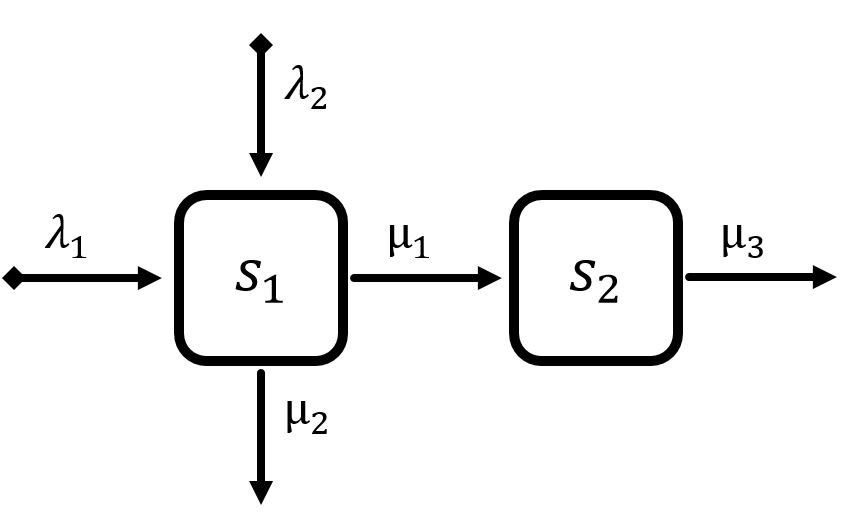
\includegraphics[width=.4\linewidth]{Paper_criss_cross.JPG}
\caption[]{The criss-cross network}
\label{fig:cc}%
\end{figure}

 We assume that the jobs of class 1 and class 2 arrive to the system following Poisson process with rate $\lambda_1$ and with rate $\lambda_2$ correspondingly. Both classes are served in the 1st server. After being served jobs of class 1 become jobs of class 3 and wait for 2nd server service. Jobs of the 2nd and 3rd classes leave the system after their service completion.
Service times are i.i.d. having exponential distribution with mean $m_j,~ j = 1, 2, 3$.



We assume that both servers employ an non-idling service policy, which means that each
server must be busy whenever there is a job available for processing. The only decision that the system manager has to make is to choose whether to process a job of class 1  or a job of class
3 if both buffers 1 and 3 are non-empty.

Let $x^j(t)$ be the number of class $j$ jobs (including possibly the one in service) in the system  at
time $t,~j = 1, 2, 3$.  We use $x(t) = \left[x^1(t), x^2(t), x^3(t)\right]$ to denote the system state at time $t$. We assume that the system manager executes a stationary Markovian policy $\pi$ i.e. the policy $\pi$ dictates a preemption-resume priority for jobs of either class 1 or class 3 solely based on the system state $x(t)$ at time $t$.


 The objective is to find a stationary policy that minimizes the long-run average number
of jobs in the network:

\begin{equation}\label{co}
\inf\limits_{\pi} \lim\limits_{T\rightarrow \infty} \frac{1}{T} \underset{\pi}{\E} \int\limits_0^T\Big[x^1(t)+x^2(t)+x^3(t)\Big]dt
\end{equation}

Under classical assumptions on arrival and service processes we can convert the original continuous-time problem to  an equivalent continuous-time Markov process where the average time between
transitions is constant. The problem becomes  probabilistically equivalent to   discrete-time control
problem \cite{Lippman1975}.


 We let $\nu = \lambda_1+\lambda_2 + \sum\limits_{i=1}^3 \mu_i$  denote uniform transition rate, where $\mu_i = \frac{1}{m_i}$, $i=1, 2, 3$. We can consider the equivalent discrete-time control
problem, where depending on control, $a = 1$ (class 1 has preemption-resume high priority) or $a = 2$, the transition probabilities are given by:



\begin{equation}\label{eq:pr}
        \begin{aligned}[b]
&P_{(x^1, x^2, x_3),(x^1-1, x^2, x^3) }(a=1) = \frac{\mu_1}{\nu}1_{x_1>0}\\
&P_{(x^1, x^2, x_3),(x^1, x^2-1, x^3) }(a=1) = \frac{\mu_2}{\nu}1_{x_2>0, x_1=0}\\
&P_{(x^1, x^2, x_3),(x^1-1, x^2, x^3) }(a=2) = \frac{\mu_1}{\nu}1_{x_1>0, x_2=0}\\
&P_{(x^1, x^2, x_3),(x^1, x^2-1, x^3) }(a=2) = \frac{\mu_2}{\nu}1_{x_2>0}\\
&P_{(x^1, x^2, x_3),(x^1+1, x^2, x^3) } = \frac{\lambda_1}{\nu}\\
&P_{(x^1, x^2, x_3),(x^1, x^2+1, x^3) } = \frac{\lambda_2}{\nu}\\
&P_{(x^1, x^2, x_3),(x^1, x^2, x^3-1) } = \frac{\mu_3}{\nu}
        \end{aligned}
\end{equation}

The probability of having a fictitious transition is
\begin{align*}
&P_{(x^1, x^2, x^3),(x^1, x^2, x^3) } = 1 - P_{(x^1, x^2, x^3),(x^1+1, x^2, x^3) } - \\
&\quad\quad\quad P_{(x^1, x^2, x^3),(x^1, x^2+1, x^3) } - P_{(x^1, x^2, x^3),(x^1-1, x^2, x^3) } - P_{(x^1, x^2, x^3),(x^1, x^2-1, x^3) }-P_{(x^1, x^2, x^3),(x^1, x^2, x^3-1) }
\end{align*}

The "fake" event  does not
represent any real jump in the original CTMC, but allows to unify average time between real
transitions.

We abuse the notation and denote a state  as $x(k) = [x^1_k, x^2_k, x^3_k]$ after $k$ transitions of the DTMC.


The objective (\ref{co}) is equivalent to:
\begin{equation}\inf\limits_{\pi} \sum\limits_{N\rightarrow \infty}\frac{1}{N}\underset{\pi}{\E}\left[ \sum\limits_{k=0}^{N-1}(x^1_k+x^2_k+x^3_k)\right].\end{equation}





\subsection{General formulation}




Let $L$ be a total number of services and $I$ be the total number of buffers.  We let $x(t) = [x^1(t), x^2(t), ..., x^J(t)]$ denote the number of jobs of each class $i$ at time $t$ in the system, including a job that might be in service. We interpret $s(i)$ as the server associated with job class $i$. We define $B_l = \{j, j=1, .., J:~ s(j)  = l\}$ as a set of classes that are processed by server $l$. We assume that routing in the network can be probabilistic: after being served  job of class $j$ becomes job of  class $k$ with probability $u_{jk}$ and leave the network with probability $1 - \sum\limits_{k=1}^K u_{jk}.$ We let $J\times J$ matrix $U = (u_{mn})_{m,n=1,..., J}$ denote the routing probabilities. External arrival processes are Poisson with rate $\lambda_j$ for jobs of class $j$, $j=1, .., J$. If no  external arrivals enter $j$th buffer we take $\lambda_j=0$. Class $j$ service times are i.i.d. having exponential
distribution with mean $1/\mu_j$, $j=1, ..., J$.


For each class $j = 1, .., J$, let $\alpha_j$ be the total arrival rate
into buffer $j$, that besides external arrivals involves transitions of jobs into class $j$ from
other classes. The vector $\alpha = [\alpha_1, \alpha_2, ..., \alpha_J]$ satisfies the following system of linear
equations, usually called as traffic equations: \begin{equation}\alpha = \lambda +U^T\alpha.\end{equation} We define the utilization of server $l$ as \begin{equation}\rho_l = \sum\limits_{j\in B_l} \frac{\alpha_j}{\mu_j}.\end{equation}
We assume that $\rho_l<1$ for all  services $l = 1, ..., L$.

 The objective is to find a stationary Markovian policy  $\pi$ that   minimize the expected long-run average number of jobs in the system:

\begin{equation}
 \inf\limits_\pi \lim\limits_{T\rightarrow \infty} \frac{1}{T} \E_{\pi}\Big[\int\limits_{0}^{T-1}\sum\limits_{j=1}^J x^j(t)dt\Big]
\end{equation}


We use uniformization to formulate MDP problem with state space $X = \mathbb{Z}_+^J$.

%We let $\nu = \sum\limits_{i=1}^I \lambda_i + \sum\limits_{i=1}^I \mu_i$  denote uniform transition rate.
We let $a_j(k)$  denote a control at $k$th decision epoch that provides priority to $j$th class, i.e. $a_j(k)=1$ means that class $j$ has the priority over other associated to server $s(j)$ classes to be served right after $k$th decision epoch. We note that $\sum\limits_{j \in B_l} a_j(k)=1$ for each server $l=1, .., L$ at each time-step $k=0, 1, 2....$  We denote the action space of the MDP problem as $A$.


The objective of the MDP problem  is to find a stationary Markovian policy $\pi:X\rightarrow A$ that minimizes long-run average number of jobs in the system, namely:

\begin{equation}
 \inf\limits_\pi \lim\limits_{N\rightarrow \infty} \frac{1}{N} \E_{\pi}\Big[\sum\limits_{k=0}^{N-1}\sum\limits_{j=1}^J x^j(k)\Big]
\end{equation}





\section{Reinforcement learning approach for queuing network control}

The undeniable success of RL has been reached for games \cite{Mnih2015}, \cite{Bellemare2013}, and physics engines \cite{Duan2016},  \cite{Todorov2012}. These problems are episodic in nature and have long but finite horizon. In the game domain each new episode (game) may require a different amount of time for the player to finish. To compare the effect of different strategies  the objective is
normalized by discounting future costs.
  Many algorithms, including TRPO and PPO, have been designed to optimize the infinite horizon discounted total cost.

In some domains, for example stochastic processing networks, it is more appropriate to optimize the long-run average cost. In this section we propose a version of  Proximal Policy Optimization algorithm which is appropriate to optimize  the long-run average performance.

\subsection{Some results from Markov chains theory}\label{sec:MC}

Let $\X$ be a countable state space and $\M_{\X, \X}$ be a set of all matrices on the countable space $\X\times \X$.



For a vector $\nu$ on $\X$, we define $\V$-weighted norm w.r.t. a vector $\V:\X\rightarrow [1, \infty)$: 

\begin{align*}
%&||\nu||_{1, \V} = \sum\limits_{x\in X} |\nu(x)|\V(x)\\
& ||\nu||_{\infty, \V} := \sup\limits_{x\in X} \frac{| \nu(x)|}{\V(x)}\\
\end{align*}



By Lemma \ref{lem:norms}  in Section \ref{sec:proofs} the corresponding induced $\V$-weighted operator norm for any matrix $M$ on $\X\times \X$ is given by
 \begin{align*}
 ||M||_V = \sup\limits_{x\in \X} \frac{1}{\V(x)}\sum\limits_{y\in \X}|M(x, y)| \V(y)
\end{align*}

We note that for any matrices $A, B, C \in \M_{\X\times \X}$ s.t. $||A||_\V<\infty, ||B||_\V<\infty, ||C||_\V<\infty$

commutativity
\begin{align*}
(A+B)C = AC +BC\quad \quad A(B +C)= AB +AC
\end{align*}
and associativity 
\begin{align*}
ABC =(AB)C= A(BC)
\end{align*}
properties hold, see \cite[Proposition 2.1, Lemma 2.1]{Jiang2017}.

%Let $\F_{1, \V}$ denote the Banach space of finite measures  on $\X$, i.e. $\nu\in \F_{1, \V}$ if and only if $||\nu ||_{1, \V}<\infty$. A bilinear mapping $T:\X\times \X \rightarrow \R$ determines a function $\nu T: \X \rightarrow\R$ whose value at point $y\in\X $ equals $[\nu T](y) := \sum\limits_{x\in \X} T(x, y) \nu(x)$. We also denote by $\F_{\infty, V}$ 
%the  space of measurable bounded functions on $X$, i.e. $f\in \F_{\infty, \V}$ if and only if $||f||_{\infty, \V}<\infty$. We define a function $Tf:\X\rightarrow \R$ for $f\in \F_{\infty, \V}$ as $ [Tf](x) := \sum\limits_{y\in \X} T(x, y) f(y).$

%Note, $|\nu^T M h|\leq ||\nu||_{1, \V}||M||_\V||h||_{\infty, \V}$ and $||M_1 M_2 ||_\V\leq ||M_1||_\V||M_2||_\V$ for any vectors $\nu, h:\X\rightarrow \R$ and  any matrices  $M_1, M_2\in \M_{\X, \X}$.
Consider an irreducible Markov chain on a countable state space $\X$ with a transition matrix $P\in   \M_{\X, \X}$. We denote $P(y|x)$ the transition probability from state $x\in \X$ to state $y\in \X$. 

Assume that there exists a vector $\V:\X\rightarrow [1, \infty)$ s.t. the following drift condition holds for some constants  $b<1$, $d\geq0$ and a finite subset $C\subset \X$:
\begin{align}\label{eq:drift}
\sum\limits_{y\in \X}P(y|x)\V(y)\leq b \V(x) +d\I_{C}(x), \quad \text{for each }x\in \X,
\end{align}
where $\I_{C}(x)=1$ if and only if $x\in C$, otherwise $\I_{C}(x)=0$.

Then the Markov chain with the transition matrix  $P$ is positive recurrent with a unique stationary distribution   $\mu$ \cite[Theorem 11.3.4]{Meyn2009}. 
By \cite[Theorem 14.3.7]{Meyn2009} we have \begin{align*}\mu^T\V <\infty, \end{align*}
where  for any function $f: \X \rightarrow \R$  we define $\mu^T f$ as
\begin{align*}
\mu^Tf:=\sum\limits_{x\in \X} \mu(x)f(x).
\end{align*}

 Vector $\V$ in the drift condition (\ref{eq:drift}) is called a \textit{Lyapunov function} for the Markov chain.



An irreducible, aperiodic Markov chain with a transition matrix  $P$ is called   \textit{$\V$-uniformly ergodic} if 
\begin{align*}||P^n - \Pi||_\V\rightarrow 0 \text{ as } n\rightarrow \infty,\end{align*} 
where every row of $ \Pi$ equals to the stationary distribution $\mu$, i.e. $\Pi(x, y): = \mu(y),$ for any $x, y\in \X.$
 


The drift condition (\ref{eq:drift}) is sufficient and necessary for an irreducible, aperiodic Markov chain  to be $\V$-uniformly ergodic \cite[Theorem 16.0.1]{Meyn2009}.

We define a cost function $g:\X \rightarrow \R$ s.t. $\mu^T |g|<\infty$ and consider the following equation:
\begin{align}\label{eq:Poisson}
g(x) - \mu^T g + \sum\limits_{y\in \X}P(y|x) h(y) - h(x) =0, \text{ for each }x\in \X,
\end{align}

Equation (\ref{eq:Poisson}) is called a \textit{Poisson's equation} of the Markov chain with transition matrix $P$ and cost function $g $. Function $h:\X\rightarrow \R$ that satisfies (\ref{eq:Poisson}) is called a \textit{solution to Poisson's equation}.  One can note that if some vector $h$ is a solution to Poisson's equation (\ref{eq:Poisson}), then for any $b\in \R$ vector $h+be$ is also a  solution to the Poisson's equation.  For example, a  solution can be defined w.r.t. any positive recurrent state. 



\begin{lemma}\label{lem:poisson_sol2}

Consider $\V$-uniformly ergodic  Markov chain with transition matrix $P$ and the stationary  distribution $\mu$. Let $x^*\in X$ be an arbitrary state of the positive recurrent Markov chain. 

 For any cost function $g:\X \rightarrow \R$ s.t. $|g|\leq \V$, the Poisson's equation (\ref{eq:Poisson}) admits a unique solution 
\begin{align}\label{eq:h2}
h^{(x^*)}(x) : = \E \left[\sum\limits_{k=0}^{\sigma(x^*)-1} \left(g(x_k) - \mu^Tg\right)\Big|~x_0 = x\right] ~\text{for each }x\in \X,
\end{align}
where $\sigma(x^*) = \min\{k>0|~x_k = x^*\}$ is the first future time when state $x^*$ is visited. 
 
 Furthermore, the solution has a finite $\V-$weighted norm: $||h^{(x^*)}||_{\infty, \V}<\infty.$
\end{lemma}
The  proof of Lemma \ref{lem:poisson_sol2} is given in \cite[Proposition A.3.1]{Meyn2007}.  We will  refer to state $x^*$ as a \textit{regeneration state}, and to the times $\sigma(x^*)$ when the regeneration state is visited   as \textit{regeneration times}. 



A solution to Poisson's equation $h$ is called a \textit{fundamental solution} if   $ \mu^T h =0.$    The proof of the following lemma is provided in \cite[Proposition A.3.11]{Meyn2007}.



\begin{lemma}\label{lem:poisson_sol}

Consider $\V$-uniformly ergodic  Markov chain with transition matrix $P$ and the stationary  distribution $\mu$.

 For any cost function $g:\X \rightarrow \R$ s.t. $|g|\leq \V$, the Poisson's equation (\ref{eq:Poisson}) admits a unique fundamental solution 
\begin{align}\label{eq:h}
h^{(f)}(x) : = \E \left[\sum\limits_{k=0}^\infty \left(g(x_k) - \mu^Tg\right)|x_0 = x\right] ~\text{for each }x\in \X,
\end{align}
where $x_k$ is the state of the Markov chain at time $k$.


\end{lemma}

Let $e = (1, 1,.., 1, ...)^T$ be a unit vector. It follows from Lemma \ref{lem:poisson_sol} that   equation  \begin{align*}(I-P+\Pi) h = g -(\mu^T g) e\end{align*}  has a unique solution whenever $|g|\leq \V$.  We can define a \textit{fundamental matrix} $Z$ that maps any cost function $|g|\leq \V$ into a corresponding fundamental solution $h^{(f)}$ as
 \begin{align}\label{eq:Zs}Z :=\sum\limits_{k=0}^\infty \left( P-\Pi \right)^k \end{align} 
s.t. the fundamental solution  (\ref{eq:h}) is equal to $h^{(f)} = Z\left(g -(\mu^T g) e\right).$ It follows from  \cite[Theorem 16.1.2]{Meyn2009} that the series (\ref{eq:Zs}) converges in $\V$-weighted norm and, moreover,  $||Z||_\V<\infty$.

We want to note that if $h_1$ and $h_2$ are two solutions to Poisson's equation (\ref{eq:Poisson}) with $\mu^T(|h_1|+|h_2|)<\infty$, then there exists a constant $b\in \R$ s.t. $h_1(x) = h_2(x) +b$ for each $x\in \X$, see \cite[Proposition 17.4.1]{Meyn2009}. For example, for any regeneration state $x^*\in \X$:
\begin{align}\label{eq:hh}
h^{(x^*)}(x) = h^{(f)}(x) -  h^{(f)}(x^*) ~\text{for each }x\in \X.
\end{align}








%Suppose that a constant $G\in \R$ and function $h:\X \rightarrow \R$ satisfy equation (\ref{eq:Poisson}). Then $G = \mu(g)$ and there exists a constant $k\in \R $ s.t. $h = Z(g - \Pi g) + k e$ where $e = (1, 1,.., 1, ...)^T.$ Moreover, for any $k\in \R$ if  $h$ satisfies (\ref{eq:Poisson}) with $G=\mu(g)$ then $h^*: = h+ ke$ also satisfies the Poisson's equation with $G = \mu(g)$, but if $\mu(h)=0$ then $h = Z(g - \Pi g)$ \cite[Section 9]{Puterman2005}. 
%
%
%First, we define the inverse of the operator $I-P+\Pi$ on $F_{1, \V}$ space. We note that for any $||\nu||_{1, \V}<\infty $, $ \nu(I-P+\Pi)=0$ implies $\nu= 0$ and the boundedness directly  follows from (\ref{eq:drift}).

%We   define  the fundamental matrix  \begin{align*}Z:=(I-P+\Pi)^{-1},  \end{align*}   and it is a bounded linear operator from space $F_{1, \V}$ to itself.
%
%
%We can also consider the inverse of the operator $I-P+\Pi$ on $F_{\infty, \V}$ space. One can observe that for any $||h||_{\infty, \V}<\infty $ equation 
%\begin{align*}
%h(x) - \sum\limits_{y\in \X} P(y|x)h(y) + \mu(h) = 0, \text{ for each }x\in \X
%\end{align*} 
%has a unique solution $h= 0.$ The boundedness $|| (I-P+\Pi)h ||_{\infty,\V}<\infty$ for any $||h||_{\infty, \V}<\infty$ follows from the drift condition (\ref{eq:drift}) and  \cite[Theorem 2.3]{Glynn1996}. 
%Hence, the operator $ (I-P+\Pi)^{-1}$ is well-defined bounded linear transformation from $F_{\infty, \V}$ to itself.  



 \subsection{Improvement guarantee for average cost objective}\label{sec:TRPOforAC}

Consider a MDP problem with a countable state space $\X$, finite action space $\A$, one-step cost function $g(x)$ and  transition function $P(\cdot|x, a)$. We assume that for each state-action pair $(x, a)$ the number of distinguish states where the chain can transit is finite, i.e. set $\{y\in \X: P(y| x, a)>0\}$ is finite for each $(x, a)\in \X\times \A.$


Suppose that $\{\theta\in \Theta\}$ denotes some open subset of Euclidean space. With every $\theta\in \Theta,$ we associate a randomized Markovian policy $\pi_{\theta}$, which at any state $x\in \X$ chooses action $a\in \A$ with probability $\pi_\theta(a|x)$. The corresponding family of  transition kernels is given by
\begin{align*}\left\{P_\theta(\cdot|x) :~P_\theta(\cdot|x) = \sum\limits_{a\in A} \pi(a|x)P(\cdot|x, a),~ \theta\in \Theta\right\}.\end{align*} 
We assume that each of the resulting Markov chains with transition probabilities $P_{\theta}(\cdot|x),~\theta\in \Theta$ is irreducible and aperiodic.

We also assume that there exists $\eta \in \Theta$, s.t. the drift condition (\ref{eq:drift}) is satisfied for the transition kernel $P_\eta$ with a Lyapunov function $\V:\X\rightarrow [1, \infty).$ By Lemma \ref{lem:poisson_sol}  a corresponding fundamental matrix   $Z_\eta$ is well-defined. For any cost function $|g|<V$ we denote a corresponding fundamental solution to the  Poisson's equation as $h_\eta$.    

%When  $\theta\in \Theta$ is sufficiently close to $\eta$, we can define an operator 
%\begin{align*}
%H_{\theta, \eta}: = (I- [P_{\theta} - P_{\eta}] Z_{\eta})^{-1}.
%\end{align*} 
%A sufficient condition to ensure that the inverse is well-define is $||  [P_{\theta} - P_{\eta}] Z_{\eta}||_\V < 1$. Then $H_{\theta, \eta}$ exists in the sense that  $H_{\theta, \eta}: = \sum\limits_{k=0}^\infty [P_{\theta} - P_{\eta}]^k Z^k_{\eta}.$
%
%
%Existence of operator $H_{\theta, \eta}$  guarantees that the Markov chain $P_{\theta}$ is positive recurrent and allows to find its stationary distribution.

\begin{restatable}{lemma}{st}\label{lem:st}
Assume that drift condition (\ref{eq:drift}) holds for $P_\eta$, $\eta \in \Theta$. Let some $\theta\in \Theta$ satisfies\begin{align*}||  [P_{\theta} - P_{\eta}] Z_{\eta}||_\V < 1  \end{align*} 
 
Then the Markov chain with transition matrix $P_\theta$ has a unique stationary distribution $\mu_{\theta}$.
\end{restatable}
The proof of Lemma \ref{lem:st} can be found in Section \ref{sec:proofs}.

For each policy $\pi_\theta$, $\theta\in \Theta$, s.t. the corresponding Markov chain $P_\theta$ is positive recurrent,  we consider a long-run average cost as a performance measure. Let $\mu_\theta$ be the stationary distribution of $P_\theta$, then we define the long-run average cost  objective as
\begin{align}\label{eq:ac}
 \mu_\theta^Tg  := \sum\limits_{x\in \X} \mu_\theta(x) g(x).
\end{align}
 The following theorem provides a bound on the difference of long-run average performance of policies $\pi_\theta$ and $\pi_{\eta}$. The proof of Theorem \ref{thm:main} can be found in Section \ref{sec:proofs}.



\begin{restatable}{theorem}{main}
\label{thm:main}
Suppose that the Markov chain with transition matrix $P_{\eta}$ is  an irreducible  chain s.t. the drift condition (\ref{eq:drift}) holds for some function $\V\geq1$ and the cost function satisfies $|g|<\V$. 

 For any $\theta\in \Theta$ s.t. 
\begin{align*} 
 D_{\theta,\eta} : = ||  [P_{\theta} - P_{\eta}] Z_{\eta}||_\V < 1
\end{align*}
the difference of long-run average costs of policies $\pi_\theta$ and $\pi_{\eta}$ is bounded by:



   \begin{align}\label{eq:ineq2}
\mu_\theta^Tg- \mu_\eta^Tg ~\leq~ &M_1(\theta, \eta)+  M_2(\theta, \eta),
\end{align}  
where $M_1(\theta, \eta)$, $M_2(\theta, \eta)$ are finite and equal to 
\begin{align*}
M_1(\theta, \eta) &:= \mu_{\eta}^T[ g -(\mu_\eta^Tg) e   +P_{\theta}h_{\eta} - h_{\eta} ]  \\
M_2(\theta, \eta) &:=\frac{ D_{\theta,\eta}^2}{1- D_{\theta, \eta}} ~  \left( 1+  \frac{ D_{\theta,\eta}}{(1- D_{\theta,\eta})}  (\mu_{\eta}^T\V) ||I - \Pi_\eta +P_\eta||_\V ||Z_{\eta}||_\V  \right)~|| g - (\mu_\eta^Tg) e  ||_{\infty, \V}~(\mu_{\eta}^T\V)
\end{align*}
\end{restatable}



%\begin{theorem}\label{thm:main}
%
%Suppose that the Markov chain with transition matrix $P_{\eta}$ is  an irreducible  chain s.t. the drift condition (\ref{eq:drift}) holds for some function $\V\geq1$ and the cost function satisfies $|g|<\V$. 
%
% For any $\theta\in \Theta$ s.t. 
%\begin{align*} 
% D_{\theta,\eta} : = ||  [P_{\theta} - P_{\eta}] Z_{\eta}||_\V < 1
%\end{align*}
%the difference of long-run average costs of policies $\pi_\theta$ and $\pi_{\eta}$ is bounded by:
%
%
%
%   \begin{align}\label{eq:ineq2}
%\mu_\theta^Tg- \mu_\eta^Tg ~\leq~ &M_1(\theta, \eta)+  M_2(\theta, \eta),
%\end{align}  
%where $M_1(\theta, \eta)$, $M_2(\theta, \eta)$ are finite and equal to 
%\begin{align*}
%M_1(\theta, \eta) &:= \mu_{\eta}^T[ g -(\mu_\eta^Tg) e   +P_{\theta}h_{\eta} - h_{\eta} ]  \\
%M_2(\theta, \eta) &:=\frac{ D_{\theta,\eta}^2}{1- D_{\theta, \eta}} ~  \left( 1+  \frac{ D_{\theta,\eta}}{(1- D_{\theta,\eta})}  (\mu_{\eta}^T\V) ||I - \Pi_\eta +P_\eta||_\V ||Z_{\eta}||_\V  \right)~|| g - (\mu_\eta^Tg) e  ||_{\infty, \V}~(\mu_{\eta}^T\V)
%\end{align*}
% 
%\end{theorem}

It follows from Theorem \ref{thm:main} that the negativity of the RHS of inequality (\ref{eq:ineq2}) guarantees the policy $\pi_\theta$ yields an improved performance comparing with the initial policy $\pi_{\eta}.$ 

One can get that $M_1(\theta, \eta) =O(D_{\theta, \eta})$:
\begin{align*}
|M_1(\theta, \eta)| &:= \left|\mu_{\eta}^T[ g -(\mu_\eta^Tg) e   +P_{\theta}h_{\eta} - h_{\eta} ] \right|\\
 &\leq (\mu_{\eta}^T\V)|| g - (\mu_\eta^Tg) e  +P_{\theta}h_{\eta} - h_{\eta } ||_{\infty, \V}\\
& =  (\mu_{\eta}^T\V)|| [P_{\theta} - P_{\eta}]h_{\eta} ||_{\infty, \V}\\
&= (\mu_{\eta}^T\V)|| [P_{\theta} - P_{\eta}] Z_{\eta}\left (g- (\mu_\eta^Tg) e\right) ||_{\infty, \V}\\
&\leq (\mu_{\eta}^T\V )|| g -(\mu_\eta^Tg) e ||_{\infty, \V} D_{\theta, \eta}
\end{align*}

The second term  $M_2(\theta, \eta)$ is nonnegative, but $M_2(\theta, \eta) = O(D_{\theta, \eta}^2)$, i.e. it is comparably small when policy $\pi_\eta$ has been subject to small changes.   
 
 Hence, there is a chance  to find $\theta\in \Theta$ s.t. $M_1(\theta, \eta) $ is negative and its absolute value is greater than the second term of the RHS of (\ref{eq:ineq2}) for some sufficiently  small $D_{\theta ,\eta}$. 

By minimizing  the RHS of (\ref{eq:ineq2}), we guarantee that the true objective $\eta$ is non-increasing:
\begin{align} 
\mu_\theta^Tg- \mu_\eta^Tg \leq  \min\limits_{\theta \in \Theta: ~D_{\theta, \eta}<1}[M_1(\theta, \eta) +M_2(\theta, \eta)] \leq M_1(\eta, \eta) +M_2(\eta, \eta) = 0
\end{align}


We can show that the distance $D_{\theta, \eta}$ can be controlled by the probability ratio 
$
r_{\theta, \eta}(a|x): =\frac{\pi_\theta(a|x)}{ \pi_{\eta}(a|x)}
$ between the policies:
\begin{restatable}{lemma}{policies}\label{lem:policies}
   \begin{align*}
D_{\theta, \eta} \leq   ||Z_{\eta}||_\V\sup\limits_{x\in X}    \sum\limits_{a\in A} \left| r_{\theta, \eta}(a|x)-  1 \right|    G_{\eta}(x, a),
\end{align*}

where $G_{\eta}(x, a): =   \frac{1}{\V(x)} \sum\limits_{y\in X}  \pi_{\eta}(a|x) P(y|x, a) \V(y)  .$

\end{restatable}


The proof of the lemma can be found in Appendix in Section \ref{sec:proofs}. Lemma \ref{lem:policies} implies that $D_{\theta, \eta}$ is small when $r_{\theta, \eta}(a|x)$ is close to 1 for each state-action pair $(x, a)$. Note that  $r_{\theta, \eta}(a|x) = 1$ and $D_{\theta, \eta}=0$ when $\theta=\eta.$
\subsection{Proximal Policy Optimization}
 
 


In  \cite{Kakade2002, Schulman2015} the authors propose to  fix the maximum change between policies $\pi_\theta$ and $\pi_{\eta}$ by bounding $M_2(\theta, \eta)$ term and focus  on minimizing $M_1(\theta, \eta)$.



We define a relative advantage function $A_{\theta}:\X\times \A\rightarrow \R$ of policy $\pi_\theta, $ $\theta\in \Theta$ as 
\begin{align}\label{eq:A}
	A_{\theta}(x, a): =   \underset{\substack{ x'\sim P(\cdot|x, a)}  }{\E} \left[g(x) - \mu_\theta^T g + h_{\theta} (x') -h_{\theta} (x) \right]                 
\end{align}
 

Then the first term on the RHS of   (\ref{eq:ineq2}) can be rewritten as
\begin{align}\label{eq:MA}
M_1(\theta, \eta) & =  \mu_{\eta}^T[ g -(\mu_\eta^Tg) e   +P_{\theta}h_{\eta} - h_{\eta} ]\\
 & =  \underset{\substack{ x\sim \mu_{\eta}\\ a\sim \pi_{\theta}(\cdot|x) \\ x'\sim P(\cdot|x, a)}  }{\E} \left[    g(x ) -(\mu_\eta^Tg) e   + h_{\eta}(x') - h_{\eta}(x)   \right]  \nonumber\\         
 &=  \underset{\substack{ x\sim \mu_{\eta}\\ a\sim \pi_{\theta}(\cdot|x)  }  }{\E} A_{\eta} (x, a)\nonumber\\
	& =  \underset{\substack{ x\sim \mu_{\eta}\\ a\sim \pi_{\eta}(\cdot|x)  }  }{\E} \left[ \frac{\pi_{\theta}(a|x)}{\pi_{\eta}(a|x)}A_{ \eta} (x, a) \right]\nonumber\\  \nonumber  
 \end{align}


 


We want to accomplish two goals: keep the ratio $r_{\theta, \eta}(a|x) =\frac{\pi_{\theta}(a|x)}{\pi_{\eta}(a|x)} $ close to 1 and minimize    \begin{align*}M_1(\theta, \eta) =  \underset{\substack{ x\sim \mu_{\eta}\\ a\sim \pi_{\eta}(\cdot|x)  }  }{\E}  r_{\theta, \eta}(a|x)A_{\eta} (x, a).\end{align*}


In \cite{Schulman2017} the authors propose the clipped surrogate objective which is minimized  w.r.t. $\theta\in \Theta$:

\begin{align}\label{eq:PO}
L(\theta, \eta):=\underset{\substack{ x\sim \mu_{\eta}\\ a\sim \pi_{\eta}(\cdot|x)  }  }{\E}   \max \left[  r_{\theta, \eta}(a|x) A_{\eta} (x, a) ,  ~ \text{clip} (r_{\theta, \eta}(a|x),  1-\epsilon, 1+\epsilon)  A_{\eta} (x, a)  \right],
\end{align}
where $\text{clip}(c,  1-\epsilon, 1+\epsilon):= \begin{cases} 1-\epsilon,~\text{ if } c<1-\epsilon,\\   1+\epsilon,~\text{ if } c>1+\epsilon,\\ c, ~\text{otherwise}\end{cases}$ for some $\epsilon\in(0, 1).$

The objective term $\text{clip} (r_{\theta, \eta}(a|x),  1-\epsilon, 1+\epsilon)  A_{\eta} (x, a) $ penalizes changes to the policy that move $ r_{\theta, \eta}(a|x) $ far  from 1. Then the final objective (\ref{eq:PO}) is   a upper bound (i.e., a pessimistic bound)   on the unclipped objective.   Thus, the objective makes $M_1(\theta, \eta)$ improve only within $\theta\in \Theta$  s.t. $r_{\theta, \eta}\in (1-\epsilon, 1+\epsilon)$.

Several alternative heuristics  have been proposed  in the literature (see, \cite{Schulman2015, Wang2016a, Schulman2017, Wu2017}) to define a loss function which controls $M_2(\theta, \eta)$ and minimize $M_1(\theta, \eta)$ terms. We use loss function (\ref{eq:PO}) in our study because of its implementation simplicity \cite{Schulman2017}.


To compute objective function one needs to evaluate the expectation and precompute advantage function in (\ref{eq:PO}). We  use Monte-Carlo simulation method and replace the expectations in (\ref{eq:PO}) and (\ref{eq:A}) by sample averages. 

Let $\{ x_0, x_1, ... \}$ be a simulated path of a positive recurrent Markov chain with  transition matrix $P$.  Let $\sigma_n$ be the $n$th time when a regeneration state $x^*$ is visited (we omit a superscript $(x^*)$). We refer to the sequence $\{ x_{\sigma_n}, x_{\sigma_n+1}, ..,  x_{\sigma_{n+1}-1}   \}$ as the $n$th \textit{regenerative cycle}. We define the length of the  $n$th regenerative cycle $R_n$ by 
\begin{align*}
R_n := \sigma_{n+1} - \sigma_{n}.
\end{align*}

We also define 
\begin{align*}
G_n :=\sum\limits_{k=\sigma_n}^{\sigma_{n+1}-1} g(x_{k})
\end{align*}     
as a cumulative cost over $n$th regenerative cycle.

For any fixed recurrent state $x^*$ the cycle lengths $\{R_n: n\geq 0\}$ are i.i.d and we denote the mean of the cycle length as $\E R $. The cumulative costs $\{G_n: n\geq 0\}$ are  i.i.d. and  we denote the mean of the cumulative cost over a cycle as $\E G $.  By the renewal reward theorem \cite[Section VI]{Asmussen2003}, the long-run average cost $\mu^T g$, when it is finite, is equal to

\begin{align*}
\mu^T g = \frac{\E G}{\E R } 
\end{align*} 


A simulation experiment for long-run average cost estimation involves  running one full regenerative cycle, i.e. $\{x_0,  x_1, ...., x_{K-1}, x_{\sigma_1}\}$ s.t. $x_0= x^*$. From one experiment, the estimates of $\E R$ and $\E G$  are equal to $\widehat{R}^{(1)} := \sigma_1$ and  $\widehat{G}^{(1)} :=   \sum\limits_{k=0}^{K-1} g(x_{k}) $ correspondingly. If we continue the simulation and generate $N$ independent repetitions (cycles), we get the following estimates:
\begin{align*}
 \widehat{R}^{(N)}:= \frac{1}{N}\sum\limits_{n=1}^N (\sigma_{n+1} - \sigma_{n}) \quad \widehat{G}^{(N)}:= \frac{1}{N}\sum\limits_{n=1}^N \sum\limits_{k=\sigma_{n}}^{\sigma_{n+1}-1} g(x_k)
\end{align*} 

 
Then, the expected average cost can be estimated by:
\begin{align}\label{es_av}
\widehat{\mu^T  g} ^{(N)} : =\frac{\widehat{G}^{(N)}   }{ \widehat{R }^{(N)}} 
\end{align}


In further discussion we refer to the average cost estimate as $\widehat{\mu^T  g}$ without specifying the number of simulation experiment repetitions.  

 The  estimation of the advantage function (\ref{eq:A}) requires availability of $h_\eta$. Even for a known policy it is computationally intractable task to solve Poisson's equation (\ref{eq:Poisson}).  
  Let assume that a trajectory which consists of $N$ regenerative cycles have been generated and $\widehat {\mu_\eta^Tg}$ has been computed. Consider an arbitrary state $x_k$ from the generated trajectory under policy $\pi_\eta$. One-repetition estimate of  solution to Poisson's equation (\ref{eq:h2}) for a state $x_k$ visited at time $k$ is defined as
\begin{align}\label{eq:es1}
\hat h_k: =  \sum\limits_{t=0}^{\sigma(k)-1} \left(g(x_{k+t }) - \widehat {\mu_\eta^Tg}  \right) ,
\end{align}
where $\sigma(k)$  is the first time when the regeneration state $x^*$ is visited after time $k$. 
We note that the one-repetition estimate (\ref{eq:es1}) is computed every timestep.

\begin{remark}
For any state $x\in \X$ the one-repetition estimate (\ref{eq:es1}) is computed every time when the state is visited (so-called \textit{every-visit} Monte-Carlo method). One can also implement a \textit{first-visit}  Monte-Carlo method which implies that the one-repetition estimate is computed once for the first time when state $x$ is visited and next visits at state $x$ within the same cycle are ignored, e.g. \cite{Cao1999}. For more details about every-visit and first-visit Monte-Carlo methods see \cite[Section 5.1]{Sutton2018}.
\end{remark}


\begin{remark}
We want to highlight the importance of the use of  regenerative simulation  and discuss some critical disadvantages of alternative simulation schemes.  One can estimate  $h^{(f)}(x),~x\in \X$  by considering a sample path of the Markov chain $\{x_0, x_1, ...\}$ which starts at $x_0 = x$  and a stationary version of the sample path $\{y_0, y_1, ..\}$ with initial state $y_0$ sampled from the stationary distribution. Then a unbiased one-repetition estimate of the Poisson's solution  (\ref{eq:h})  at state $x$ is equal to
\begin{align*}
\hat h^{(f)}(x): = \sum\limits_{k=0}^{\sigma^{(couple)} }\left[g(x_k) - g(y_k)\right],
\end{align*}
where $\sigma^{(couple)} = \min\{k\geq 0| x_k = y_k\}$ is the time when the paths meet. Unfortunately, in practice the stationary distribution is unknown and one has to simulate stationary sample path by \textit{perfect sampling} \cite{Propp1996}, which might require tremendous computational efforts.  
Also one may attempt to estimate average performance (\ref{eq:ac}) without exploiting the regenerative structure  -- given a sample path $\{x_0, ..., x_N\}$ with an arbitrary initial distribution,  the point estimator of   average performance is defined as
\begin{align}\label{eq:es_av2}
\widehat{\mu^T  g} ^{(p)} : =\frac{1 }{N+1}\sum\limits_{k=0}^{N}g(x_k) 
\end{align}
The estimator (\ref{eq:es_av2}) is typically biased. Therefore,   if   the average cost estimate required in (\ref{eq:es1}) has been obtained based on equation (\ref{eq:es_av2}), the estimator $\hat h (x)$ returns biased estimates of the solution to Poisson's equation.  
Section 5 in \cite{Cooper2003} provides more detailed discussion  of the mentioned estimation schemes.
\end{remark}





We use   function $f_\psi:\X\rightarrow \R$ from  a family of function approximators $\{f_\psi, \psi\in \Psi \}$ to represent function $h_{  \eta}$.    A single function $f_\psi$  is chosen from $\{f_\psi, \psi\in \Psi \}$ to minimize the mean square distance to the one-repetition estimates  $\{\hat  h_k\}_{k=0}^{\sigma_N-1}:$
\begin{align}\label{eq:Vappr}
\psi^* = \arg\min\limits_{\psi \in \Psi} \sum\limits_{k=0}^{\sigma_N-1} \left ( f_{\psi}(x_{k}) - \hat h_k   \right)^2.
\end{align}
 

 \begin{remark}
One might expect that  the estimation of solution to Poisson's equation $h_\eta$ has to be done over multiple regenerative cycles before solving optimization problem (\ref{eq:Vappr}). Let $x_{k_n}$ be $n$th time in the simulation when state $x$ has been visited with $x_{k_0} := x_k$, where $x$ is an arbitrary state sampled from the generated trajectory. Let $n(x)$ be the total number of visits to state $x$ over the simulation. We define $n(x)-$repetition estimate of $h_\eta (x)$ as 
\begin{align*} 
\hat h^{(n)} (x_k): = \frac{1}{n(x_k)} \sum\limits_{i = 1}^{n(x_k)}   \sum\limits_{t=k_i }^{\sigma(x_{k_i} )-1} \left(g(x_{t }) - \widehat {\mu_\eta^Tg}  \right) ,
\end{align*}

Then the optimization problem 
\begin{align*} 
\psi^* = \arg\min\limits_{\psi \in \Psi} \sum\limits_{k=0}^{\sigma_N-1} \left ( f_{\psi}(x_{k}) -\hat h^{(n)}_\eta(x_k)   \right)^2,
\end{align*}
yields the same solution as problem (\ref{eq:Vappr}), but requires additional efforts for the repetitions averaging.

The equivalence of the optimization problems follow from the fact that for an arbitrary sequence of real numbers $a_1, ..,a_n\in \R$:

\begin{align}\label{eq:opt} 
 \arg\min_{x\in \R} \sum\limits_{i=1}^n (x-a_i)^2 =  \frac{1}{n}\sum\limits_{i=1}^n a_i 
\end{align}
 
 \end{remark}
 
 
 With available function approximation of $h_\eta$, the advantage function (\ref{eq:A}) can be estimated as
 \begin{align}\label{eq:Aes1}
 	\hat A_{\eta}(x_k, a_k): =   g(x_k) - \widehat{\mu_\eta^T g} + \sum\limits_{y\in \X} P(y|x_k, a_k) f_{\psi} (y) -  f_{\psi}(x_k) 
 \end{align}

Given a trajectory of $N$ regenerative cycles $\{x_0, a_0, x_1, a_1, ..., , x_{\sigma_N-1}, a_{\sigma_N-1}, x_{\sigma_N}\}$ which starts from the regeneration state $x_0 = x^*$ the loss function (\ref{eq:PO}) is estimated as a sample average over the cycles:
 \begin{align*}
   \hat L(\theta, \eta) = \sum\limits_{k=0}^{\sigma_N-1} \max\left[ \frac{\pi_{\theta}(a_{k}| x_{k})}{\pi_{\eta}(a_{k}|x_{k})}  \hat A_{\eta}(x_{k}, a_{k}) ,\text{clip}\left(\frac{\pi_{\theta}(a_{k}| x_{k})}{\pi_{\eta}(a_{k}|x_{k})},     1-\epsilon, 1+\epsilon \right  ) \hat  A_{\eta}(x_{k}, a_{k})  \right]
   \end{align*}

If $Q$ trajectories can be simulated in parallel, each of $q=1, .., Q$ (parallel) actors collect a trajectory  \begin{align*}\{x_{0, q}, a_{0, q}, x_{1 , q}, a_{1, q}, ...., x_{\sigma_N-1, q}, a_{\sigma_N^q-1, q}, x_{\sigma_N^q, q}\}   \end{align*} with $N$ regenerative cycles, where $\sigma_N^q$  is $N$th regeneration time in the simulation of $q$th actor and $x_{0, q} = x^*$ for each $q=1, ..., Q$. 


Each iteration  the surrogate loss is constructed based on these $\sum\limits_{q=1}^Q \sigma_N^q$ timesteps of data. Optimization of the loss function yields a new policy for the next iteration.



\begin{algorithm}[H]
\SetAlgoLined
\KwResult{policy $\pi_{\theta_I}$ }
 Initialize  policy $\pi_{\theta_0}$ and value function $f_{\psi_0}$ approximators \;
 \For{ policy iteration $i= 1, 2, ..., I$}{
  \For{ actor  $q= 1, 2, ..., Q$}{
  Run policy $\pi_{\theta_{i}}$  until it reaches $N$th regeneration time on $\sigma_N^q$ step: collect an episode
   $\{x_{0, q}, a_{0, q}, x_{1 , q}, a_{1, q}, ...., x_{\sigma_N-1, q}, a_{\sigma_N^q-1, q}, x_{\sigma_N^q, q}\} $\;
  }

  Compute average cost estimate $\widehat{\mu^T  g}$ by (\ref{es_av})\;
        Compute  $\hat h_{k, q}$,  estimate of $h_{\theta_i}(x_{k, q})$, by (\ref{eq:es1})  for each $q = 1, .., Q$, $k=1, .., \sigma_{N}^q-1$\;
        Update $\psi_{i}: = \psi$, where $\psi$ minimizes $ \arg\min\limits_{\psi \in \Psi}\sum\limits_{q=1}^Q \sum\limits_{k=0}^{\sigma_{N}^q-1 } \left ( f_{\psi}(x_{k, q}) -\hat h_{k, q}   \right)^2$ following (\ref{eq:Vappr}) \;
  Estimate advantage functions $\hat A_{\theta_{i}}(x_{k, q}, a_{k, q})$ using (\ref{eq:Aes1}) for each $q = 1, .., Q$, $k=1, .., \sigma_{N}^q-1$\;
 Minimize surrogate objective function w.r.t. $\theta\in \Theta$:
 \begin{align*}
   \hat L(\theta, \theta_i) =\sum\limits_{q=1}^Q \sum\limits_{k=0}^{\sigma^q_N-1} \max\Big[ &\frac{\pi_{\theta}(a_{k, q}| x_{k, q})}{\pi_{\theta_{i}}(a_{k, q}|x_{k, q})}  \hat A_{\theta_{i}}(x_{k, q}, a_{k, q}) ,\\ &\text{clip}\left(\frac{\pi_{\theta}(a_{k,q}| x_{k, q})}{\pi_{\theta_{i}}(a_{k, q}|x_{k, q})},     1-\epsilon, 1+\epsilon  \right) \hat A _{\theta_{i}}(x_{k, q}, a_{k,q})  \Big]
   \end{align*}
 Update $\theta_{i+1}: = \theta$
 }
 \caption{Base proximal policy optimization algorithm}\label{alg1}
\end{algorithm}

%
%\begin{remark}
%Note that the advantage function $\hat A_{\theta_{i+1}}$ is computed using $h_{\psi_{i+1}}$ which is an approximation of the value function of policy $\pi_{\theta_i}$, not $\pi_{\theta_{i+1}}$. 
%Additional bias might be introduced if the value function is updated
%first, see \cite[Section 6.1]{Schulman2016}. For example, if   $N=1$ and approximation in (\ref{eq:Vappr}) overfits the data, i.e.  $h_{\psi}(x_{k}) =\hat h_\eta(x_k)$ for each $x_k$,  then estimates of the advantage function   $\hat A_{\theta_{i+1}}$ become zero for all generated state-action pairs $(x_k, a_k)$. 
%\end{remark}

\section{Advantage function estimation}\label{sec:M1}



The main goal of the advantage function $A_{\eta} (x, a)$ is to predict the effect of action $a$ realization at state $x$. If approximation  $f_\psi$ is not sufficiently close to a true solution of  Poisson's equation, the effect of the action on the future can be evaluated incorrectly by estimator (\ref{eq:Aes1}) that can be a cause of suboptimal policy update.


% Let $x^*$ be a regeneration state. We define a   state-action relative value function $Q _{\eta} :\X\times \A\rightarrow \R$ of policy $\pi_\theta, $ $\theta\in \Theta$ as 
%
%\begin{align*} 
%Q(x, a) : = \E \left[\sum\limits_{k=0}^{\sigma(x^*)-1} \left(g(x_k) - (\mu^Tg)\right)\Big|x_0 = x\right], ~\text{for each }x\in \X
%\end{align*}
%where $x=x_0$ and action $a = a_0$ is taken at time $k=0$;  the following actions starting from time $k=1$ are taken according to policy $\pi_\theta$;  $\sigma(x^*) = \min\{k>0|x_k = x^*\}$ is the first future time when state $x^*$ is visited. 
%
%We note that  $A_{\eta}(x, a) =Q_\eta(x, a)  - h_\eta(x )  $  for each $(x, a)\in \X\times \A$. We also note that the Poisson's solution function  $h_\eta(x ) $ does not depend on  actions and serves as a normalization \textit{baseline} for the state-action value functions \cite[Section 13.4]{Sutton2018}.



\subsection{Approximating martingale-process method}

 


%One can estimate state-action function considering 
%\begin{align}\label{eq:es2}
%\hat Q (x_k, a_k): =  \sum\limits_{t=0}^{\sigma_k(x^*)-1} \left(g(x_{k+t }) - \widehat {\mu^Tg}  \right),
%\end{align}
%where $\sigma_k(x^*)$ is the first regeneration time after time $k$.

Estimator (\ref{eq:es1}) of  the solution to Poisson's equation suffers from the high variance when the regenerative cycles are long -- the sum of relative costs $g(x_k) - \mu_\eta^Tg$   becomes large before it is reset to zero at the regeneration state.   In this section we discuss how one can decrease  the variance by reducing the magnitude of summands in (\ref{eq:es1}) if  an approximation $\zeta$  of the solution to Poisson's equation $ h_\eta$ is available.

Let assume  a trajectory $\{x_0, a_1, x_1, a_2, ...., x_{K-1}, a_{K-1}, x_{\sigma_N}\}$ has been generated under policy $\pi_\eta$. From the definition of a solution to Poisson's equation (\ref{eq:Poisson}):


\begin{align*}
g(x_{k }) - \mu^Tg = \sum\limits_{y\in X} P_\eta(y| x_k) h_\eta(y) - h_\eta(x_k) \text{ for each state } x_k  \text{ in the simulated trajectory.}
 \end{align*}

If the approximation $\zeta$ is sufficiently close to $ h_\eta$, then the correlation between
\begin{align*} 
g(x_{k }) -  \widehat {\mu^Tg}  \quad \text{ and }\quad \sum\limits_{y\in X} P_\eta(y| x_k) \zeta(y) -\zeta(x_k)
\end{align*} 
is positive and the control variate method can be used to reduce the variance. This idea gives rise to the approximating martingale-process (AMP) method proposed in \cite{Henderson2002}.


Following \cite[Proposition 7]{Henderson2002} we define a martingale process $M = (M_n:n\geq 0)$ , where for $x = x_0$
\begin{align}\label{eq:M}
M_n(x) :=  \zeta(x_0)-\zeta(x_n) +\sum\limits_{k=0}^{n-1} \left[\sum\limits_{y\in \X} P_\eta(y|x_k) \zeta(y)  - \zeta(x_k)\right]
\end{align}

The martingale process (\ref{eq:M}) has zero expectation $\E M_n = 0$ for all $n\geq 0$ and can be used as a control variate.

From equality (\ref{eq:hh})  $h_\eta(x^*)=0$  and we can assume that $\zeta(x^*)=0$. Consider the martingale process starting from an arbitrary state $x_k$  until the first regeneration time:
\begin{align*}
M_{\sigma_k} (x_k)=\zeta(x_k) +\sum\limits_{t=0}^{\sigma_k-1} \left[\sum\limits_{y\in \X} P_\eta(y|x_{k+t})\zeta(y)  - \zeta(x_{k+t})\right]
\end{align*}


Then adding $M_{\sigma_k}$ to estimator (\ref{eq:es1}) we get the AMP estimator of the solution to Poisson's equation:
\begin{align}\label{eq:es2}
\hat h_\eta^{AMP(\zeta)} (x_k, a_k)&: =\zeta(x_k) +  \sum\limits_{t=0}^{\sigma_k-1} \left(g(x_{k+t }) - \widehat {\mu_\eta^Tg} +\sum\limits_{y\in \X} P_\eta(y|x_{k+t})\zeta(y) -\zeta(x_{k+t})  \right)\\
&=g(x_k) - \widehat {\mu_\eta^Tg} +\sum\limits_{y\in \X} P_\eta(y|x_{k})\zeta(y)
 +  \sum\limits_{t=1}^{\sigma_k-1} \left(g(x_{k+t }) - \widehat {\mu_\eta^Tg} +\sum\limits_{y\in \X} P_\eta(y|x_{k+t}) \zeta(y) -\zeta(x_{k+t})  \right) \nonumber.
\end{align}

Let assume that estimation of the average performance is accurate, i.e. $ \widehat {\mu_\eta^Tg}  = \mu_\eta^Tg$. In this case estimator (\ref{eq:es2}) has zero variance if the approximation is exact $\zeta = h_\eta$.



% We get the AMP  estimator of the advantage function  
%\begin{align}\label{eq:es3}
%\hat A^{AMP(\tilde h)} (x_k, a_k) &:=\hat Q^{AMP(\tilde h)}(x_k, a_k) -\tilde h(x_k) \nonumber\\
%&=  \sum\limits_{t=0}^{\sigma_k(x^*)-1} \left(g(x_{k+t }) - \widehat {\mu^Tg} +\sum\limits_{x'\in \X} P_\eta(x'|x) \tilde h(x') -\tilde  h(x_k)  \right). 
%\end{align}
 
 %The empirical evidence  of sample complexity improvement with AMP estimator is provided in Section \ref{sec:AMPexp}.  

Now we want replace the standard regenerative estimation   in line 8 of Algorithm \ref{alg1} by AMP estimator (\ref{eq:es2}). As the approximation $\zeta$ we use approximation $f_{\psi_{i-1}}$ that corresponds to preceding policy, i.e. in line 8  of Algorithm \ref{alg1} we replace $\hat h (x_k)$ by estimates $\hat h^{AMP(f_{\psi_{i-1}} )} (x_k)$ that are computed by (\ref{eq:es2}).

 
 
 
 \begin{algorithm}[H]
\SetAlgoLined
\KwResult{policy $\pi_{\theta_I}$ }
 Initialize  policy $\pi_{\theta_0}$ and value function $f_{\psi_0}$ approximators \;
 \For{ policy iteration $i= 1, 2, ..., I$}{
  \For{ actor  $q= 1, 2, ..., Q$}{
  Run policy $\pi_{\theta_{i}}$  until it reaches $N$th regeneration time on $\sigma_N^q$ step: collect an episode
   $\{x_{0, q}, a_{0, q}, x_{1 , q}, a_{1, q}, ...., x_{\sigma_N-1, q}, a_{\sigma_N^q-1, q}, x_{\sigma_N^q, q}\} $\;
  }

  Compute average cost estimate $\widehat{\mu^T  g}$ by (\ref{es_av})\;
        Compute  $\hat h^{AMP(f_{\psi_{i-1}})}_{k, q}$,  estimate of $h_{\theta_i}(x_{k, q})$, by (\ref{eq:es2})  for each $q = 1, .., Q$, $k=1, .., \sigma_{N}^q-1$\;
        Update $\psi_{i}: = \psi$, where $\psi$ minimizes $ \arg\min\limits_{\psi \in \Psi}\sum\limits_{q=1}^Q \sum\limits_{k=0}^{\sigma_{N}^q-1 } \left ( f_{\psi}(x_{k, q}) -\hat h^{AMP(f_{\psi_{i-1}})}_{k, q}   \right)^2$ following (\ref{eq:Vappr}) \;
  Estimate advantage functions $\hat A_{\theta_{i}}(x_{k, q}, a_{k, q})$ using (\ref{eq:Aes1}) for each $q = 1, .., Q$, $k=1, .., \sigma_{N}^q-1$\;
 Minimize surrogate objective function w.r.t. $\theta\in \Theta$:
 \begin{align*}
   \hat L(\theta, \theta_i) =\sum\limits_{q=1}^Q \sum\limits_{k=0}^{\sigma^q_N-1} \max\Big[ &\frac{\pi_{\theta}(a_{k, q}| x_{k, q})}{\pi_{\theta_{i}}(a_{k, q}|x_{k, q})}  \hat A_{\theta_{i}}(x_{k, q}, a_{k, q}) ,\\ &\text{clip}\left(\frac{\pi_{\theta}(a_{k,q}| x_{k, q})}{\pi_{\theta_{i}}(a_{k, q}|x_{k, q})},     1-\epsilon, 1+\epsilon  \right) \hat A _{\theta_{i}}(x_{k, q}, a_{k,q})  \Big]
   \end{align*}
 Update $\theta_{i+1}: = \theta$
 }
 \caption{Proximal policy optimization with AMP method}\label{alg1amp}
\end{algorithm}




\subsection{Generalized  estimation}

In the previous section we applied AMP method to reduce the variance  of the summands in (\ref{eq:es1}). Unless an approximation $\zeta$ is exact, each term in  the summation in (\ref{eq:es2}) is random with nonzero variance.  When the expected length of a regeneration cycle is large the   cumulative variance  in estimator (\ref{eq:es2}) still can be devastating.
 

The common approach to overcome this issue  is to introduce a forgetting   factor $\gamma<1$
 to discount the future relative costs  \cite{Jaakkola1994, Baxter2001, Marbach2001, Kakade2001, Thomas2014, Schulman2016}. % When a regeneration cycle are long and in average its length $\E G$ is large   one may sum relative costs $g(x_k) - \mu^Tg$ up to some fixed timestep $N$ in estimator (\ref{eq:es1})  s.t. $N<\E G$. The choice of $N$ can be generalized assuming that the
 % number of summands $N$  follows geometrical distribution with parameter $\gamma<1$ as in TD($\lambda$) method \cite[Section 12]{Sutton2018}.   }
We approximate solution of Poisson's equation $h_{\eta}$ by a corresponding infinite-horizon discounted relative value function:
\begin{align*}
J_{\eta}^{(\gamma)}(x): = \E \left[ \sum\limits_{t=0}^\infty \gamma^{t+1}  (g(x_t) - \mu^T_\eta g ) \Big| x_0 = x\right] \text{ for each }x\in \X,
\end{align*}
 where  $x_k$ is the state of the Markov chain $P_\eta$ at time $k$ and  $\gamma<1$ is a discount factor.

We note that $J^{(\gamma)}_{\eta} \rightarrow h_\eta$  in $\V$-weighted norm as $\gamma\rightarrow 1$  for $\V$-uniformly ergodic Markov chain, see Lemma \ref{lem:disc}.

 

%The variance reduction from the discounting  has been analyzed in \cite[Section 5.4.2]{Marbach1998a} for a finite state space.

Now we replace $h_\eta$ by $J^{(\gamma)}_{\eta}$ in the expression for $M_1(\theta, \eta)$:
\begin{align*}
M^{(\gamma)}_1(\theta, \eta):=\mu_{\eta}^T( g - \mu_\eta^T g e + P_{\theta}  J^{(\gamma)}_{\eta} - J^{(\gamma)}_{\eta}  )
\end{align*}

We define an infinite-horizon discounted   value function 
\begin{align*}
V^{(\gamma)}_{\eta}(x): = \E \left[ \sum\limits_{t=0}^\infty \gamma^{t }  g(x_t)  \Big| x_0 = x\right] \text{ for each }x\in \X,
\end{align*}

and note that $J^{(\gamma)}_{\eta}(x) = \gamma V^{(\gamma)}_{\eta}(x) + \frac{\gamma}{1-\gamma}\mu^T_\eta g$ for each $x\in \X.$

The optimization problem (\ref{eq:ineq2}) searches $\theta \in \Theta$  s.t. $M_1(\theta, \eta)+M_2(\theta, \eta)$   is minimized. Its solution can be approximately found minimizing $\mu^T_{\eta}( g   +\gamma P_{\theta}V^{(\gamma)}_{\eta} -   V^{(\gamma)}_{\eta} ) +M_2(\theta, \eta)$ since
\begin{align*}
\arg\min\limits_{\theta\in \Theta} [M_1(\theta, \eta)+M_2(\theta, \eta) ] & \approx \arg\min\limits_{\theta\in \Theta} [M^{(\gamma)}_1(\theta, \eta)+M_2(\theta, \eta) ]  \\
&= \arg\min\limits_{\theta\in \Theta}\left[\mu_{\eta}^T( g - \mu_\eta^T g e + P_{\theta}J^{(\gamma)}_{\eta} - J^{(\gamma)}_{\eta}  +M_2(\theta,  \eta) \right]\\
&= \arg\min\limits_{\theta\in \Theta}\left[\mu_{\eta}^T( g - \mu_\eta^T g e + \gamma P_{\theta} V^{(\gamma)}_{\eta}  - \gamma V^{(\gamma)}_{\eta}  ) +M_2(\theta,  \eta) \right]\\
&= \arg\min\limits_{\theta\in \Theta}\left[\mu_{\eta}^T( g  + \gamma P_{\theta} V^{(\gamma)}_{\eta}  -  V^{(\gamma)}_{\eta}  ) +M_2(\theta,  \eta) \right]\\
\end{align*}



  We define an infinite-horizon discounted advantage function $A_{\theta}^{ (\gamma)}:\X\times \A\rightarrow \R$ of policy $\pi_\theta, $ $\theta\in \Theta$ as 
\begin{align}\label{eq:A2}
	A_{\theta}^{ (\gamma)}(x, a): =   \underset{\substack{ x'\sim P(\cdot|x, a)}  }{\E} \left[g(x) +\gamma V^{(\gamma)}_{\theta}(x') - V^{(\gamma)}_{\theta} (x) \right]                 
\end{align}
Let episode $\{x_0, a_0, ...,x_{N_1} ,a_{N-1}\}$ be generated by policy $\pi_\eta$. With available approximation  $f_\psi$ of the  discounted value function $V^{(\gamma)}_\eta$, the advantage function (\ref{eq:A2}) can be estimated as
 \begin{align}\label{eq:Aes2}
 	\hat A^{(\gamma)}_{\eta}(x_k, a_k): =   g(x_k)  +\gamma \sum\limits_{y\in \X} P(y|x_k, a_k) f_{\psi} (y) -  f_{\psi}(x_k), 
 \end{align}
 for each state-action pair $(x_k, a_k)$ from the generated episode.
 
Then we can rewrite $M_1^{(\gamma)}(\theta, \eta)$ using an advantage function definition following  (\ref{eq:MA}):
\begin{align*}
	M_1^{(\gamma)}(\theta, \eta) & = \mu_{\eta}^T( g + \gamma P_{\theta}V^{(\gamma)}_{\eta} - V^{(\gamma)}_{\eta})\\
	& =  \underset{\substack{ x\sim \mu_{\eta}\\ a\sim \pi_{\eta}(\cdot|x)  }  }{\E}  \left[\frac{\pi_{\theta}(a|x)}{\pi_{\eta}(a|x)}A_{\eta}^{ (\gamma)} (x, a)\right]\\
\end{align*}


The PPO loss function becomes:
\begin{align}\label{eq:PO2}
L^{(\gamma)}(\theta, \eta):=\underset{\substack{ x\sim \mu_{\eta}\\ a\sim \pi_{\eta}(\cdot|x)  }  }{\E}   \max \left[  r_{\theta, \eta}(a|x) A^{(\gamma)}_{\eta} (x, a) ,  ~ \text{clip} (r_{\theta, \eta}(a|x),  1-\epsilon, 1+\epsilon)  A^{(\gamma)}_{\eta} (x, a)  \right].
\end{align}



The AMP estimator for the discounted value function can be derived following the procedure in the previous section. The details can be found in Appendix in Section \ref{sec:AMPforDisc}.
Let $\zeta$ be an approximation of the discounted value function. We get the corresponding AMP  estimator for  $V^{(\gamma)}_\eta(x_k)$:  
\begin{align}\label{eq:es4}
\hat V_k^{AMP(\zeta), (\gamma)}:=  g(x_k )+  \gamma \sum\limits_{y\in X} P_{\eta}(y|x_k)  \zeta(y) + \sum\limits_{k=1}^\infty\gamma^k \left(g(x_k ) +  \gamma \sum\limits_{y\in X} P_{\eta}(y|x_k)  \zeta(y)   -   \zeta(x_k )  \right)  
\end{align}
Similarly to (\ref{eq:es2}), estimator (\ref{eq:es4}) has zero variance if approximation of the discounted value function is exact $\zeta = V _\eta.$

Further variance reduction in discounted value function estimation is possible when the summation in (\ref{eq:es4}) is done only for the next $T$ timesteps after time $k$.  Generalizing this choice one can assume that the
  number of summands $T$  follows geometrical distribution with parameter $\lambda<1$ as in TD($\lambda$) method \cite[Section 12]{Sutton2018}. We use a truncated version of TD$(\lambda)$ which reduces to
(\ref{eq:es4}) when $\lambda=1$ and $N=\infty$:
\begin{align}\label{eq:esf}
\hat V^{AMP( \zeta), (\gamma, \lambda)}_k  :=g(x_k )+  \gamma \sum\limits_{y\in X} P_{\eta}(y|x_k)  \zeta(y) + \sum\limits_{t=1}^{N-k} (\gamma\lambda)^k \left(g(x_{k+t}) +  \gamma \sum\limits_{y\in X} P_{\eta}(y|x_{k+t})  \zeta(y)   -   \zeta(x_{k+t})  \right). 
\end{align}
 
 
We provide the proximal policy optimization algorithm where each of $q=1, .., Q$ parallel actors simulate an episode with length $N$: $\{x_{0, q}, a_{0,q}, x_{1, q}, a_{1, q}, ...., x_{N-1, q}, a_{N-1, q} \}.$  Formula (\ref{eq:esf})  is used to estimate discounted value function values for each state $x_{k,q}$ in the simulated data. As the approximation $\zeta$ we use approximation of the discounted value function of the preceding policy $\zeta = f_{\psi_{i-1}},  $ see Algorithm \ref{alg2}.
 
\begin{algorithm}[H]
\SetAlgoLined
\KwResult{policy $\pi_{\theta_I}$ }
 Initialize  policy $\pi_{\theta_0}$ and value function $f_{\psi_0}$ approximators \;
 \For{ policy iteration $i= 1, 2, ..., I$}{
  \For{ actor  $q= 1, 2, ..., Q$}{
  Run policy $\pi_{\theta_{i}}$  for $N$ timesteps: collect an episode
   $\{x_{0, q}, a_{0, q}, x_{1 , q}, a_{1, q}, ...., x_{ N-1, q}, a_{N-1, q}, x_{N, q}\} $\;
  }
 
        Compute  $\hat V^{AMP( f_{\psi_{i-1}}), (\gamma, \lambda)}_{k, q}  $ estimates by (\ref{eq:esf})  for each $q = 1, .., Q$, $k=1, .., N-1$\;
        Update $\psi_{i}: = \psi$, where $\psi$ minimizes $ \arg\min\limits_{\psi \in \Psi}\sum\limits_{q=1}^Q \sum\limits_{k=0}^{N-1 } \left ( f_{\psi}(x_{k, q}) -\hat V^{AMP(  f_{\psi_{i-1}}), (\gamma, \lambda)}_{k, q} \right)^2$ following (\ref{eq:Vappr}) \;
  Estimate advantage functions $\hat A^{(\gamma)}_{\theta_{i}}(x_{k, q}, a_{k, q})$ using (\ref{eq:Aes2}) for each $q = 1, .., Q$, $k=1, ..,N-1$\;
 Minimize surrogate objective function w.r.t. $\theta\in \Theta$:
 \begin{align*}
   \hat L^{(\gamma)}(\theta, \theta_i) =\sum\limits_{q=1}^Q \sum\limits_{k=0}^{ N-1} \max\Big[ &\frac{\pi_{\theta}(a_{k, q}| x_{k, q})}{\pi_{\theta_{i}}(a_{k, q}|x_{k, q})}  \hat A^{(\gamma)}_{\theta_{i}}(x_{k, q}, a_{k, q}) ,\\ &\text{clip}\left(\frac{\pi_{\theta}(a_{k,q}| x_{k, q})}{\pi_{\theta_{i}}(a_{k, q}|x_{k, q})},     1-\epsilon, 1+\epsilon  \right) \hat A ^{(\gamma)}_{\theta_{i}}(x_{k, q}, a_{k,q})  \Big]
   \end{align*}
 Update $\theta_{i+1}: = \theta$
 }
 \caption{Proximal policy optimization with discounting}\label{alg2}
\end{algorithm}




\section{Experimental results for multiclass queuing networks}\label{sec:experiments}
In this section we evaluate performance of the proposed proximal policy optimization Algorithms \ref{alg1},  \ref{alg1amp} and \ref{alg2} for multiclass queuing networks control optimization task discussed in Section \ref{sec:MQN}. 
 

 

We use two separate fully-connected feed-forward neural networks to represent  policies $\pi_\theta,$ $\theta\in \Theta$ and value functions $f_\psi$, $\psi\in \Psi$ with the architecture details provided in Section \ref{sec:nn} in Appendix.  We will refer to the neural network used to represent a policy as \textit{the  policy NN} and to  the neural network used to approximate a value function as \textit{the value function NN}. In each experiment we run the algorithm for $I=200$ iterations. Each iteration the algorithm uses $Q=50$ actors to simulate data in parallel.    See Section \ref{sec:par} in the
Appendix for more details on the experimental setup and hyperparameters. 



\subsection{Criss-cross network}

 We first study PPO algorithm and compare its base version Algorithm \ref{alg1} and its modification Algorithm \ref{alg1amp} that incorporates the  AMP method.  We check the robustness of the algorithms for the criss-cross system  with  various load (traffic) intensity regimes, including    I.L. (imbalanced light), B.L. (balanced light), I.M. (imbalanced medium), B.M. (balanced medium), I.H. (imbalanced heavy), and B.H. (balanced heavy) regimes.   The corresponding arrival and service rates are presented in Table \ref{t:lp}. The criss-cross network executed with any of these traffic regimes is stable under any work-conserving policy  \cite{Dai1996}.






We summarize control policies that have been proposed in the literature in Table \ref{tab:cc}. In the first column of Table \ref{tab:cc} we indicate the load regime. In the second column we report the optimal performance obtained via dynamic programming, denoted by DP.  In the third column
we report the performance of a target-pursuing
policy proposed in \cite{Paschalidis2004} and denoted by OTP in the table. In the fourth column we list the performance of a threshold policy proposed in \cite{Harrison1990}.
 In the fifth and sixth columns
we list the performance of fluid (FP) and robust fluid (RFP) policies from  \cite{Bertsimas2015}.

In the last column of Table \ref{tab:cc} we provide simulation results of PPO policy $\pi_{\theta_I}$ obtained from Algorithm \ref{alg1amp}. We want to highlight that we report the performance of the policy resulting from the \textit{last} iteration of the algorithm, which might be not the best policy over the course of learning. 

The policy NN parameters $\theta_0$ are initialized using standard Xavier initialization \cite{Glorot2010}.  The resulting policy $\pi_{\theta_0}$ is close to the policy that chooses actions uniformly at random.  We take the empty system state $x^* = (0,0,0)$ as a regeneration state and simulate $N=5000$ independent regenerative cycles  per actor in each iteration of the algorithm. Although the number of generated cycles is fixed for all traffic regimes, the length of regenerative cycles varies  and highly depends on the load. 

In order to present the learning curves in Figure \ref{fig:cc_opt}  we  save policy parameters $\{\theta_i\}_{i=0, 10, ..., 200}$ every 10th iteration over the course of learning. After the algorithm terminates we independently 
 simulate   policies $\{    \pi_{\theta_i}: i = 0, 10, ..., 200 \}$  starting from the regeneration state $x = (0,..,0)$ until fixed number of regenerative events happened. For light (medium, heavy)  traffic regime the simulation is run for $10^7$ ($5\times 10^6$, $10^6$) regenerative cycles correspondingly. 
  $95\%-$confidence intervals   are computed using the strongly consistent estimator of asymptotic variance, see details in \cite[Section VI.2d]{Asmussen2003}.


  \begin{figure}[H]
    \subfloat[Imbalanced low (IL) traffic \label{subfig-6:IL}]{%
       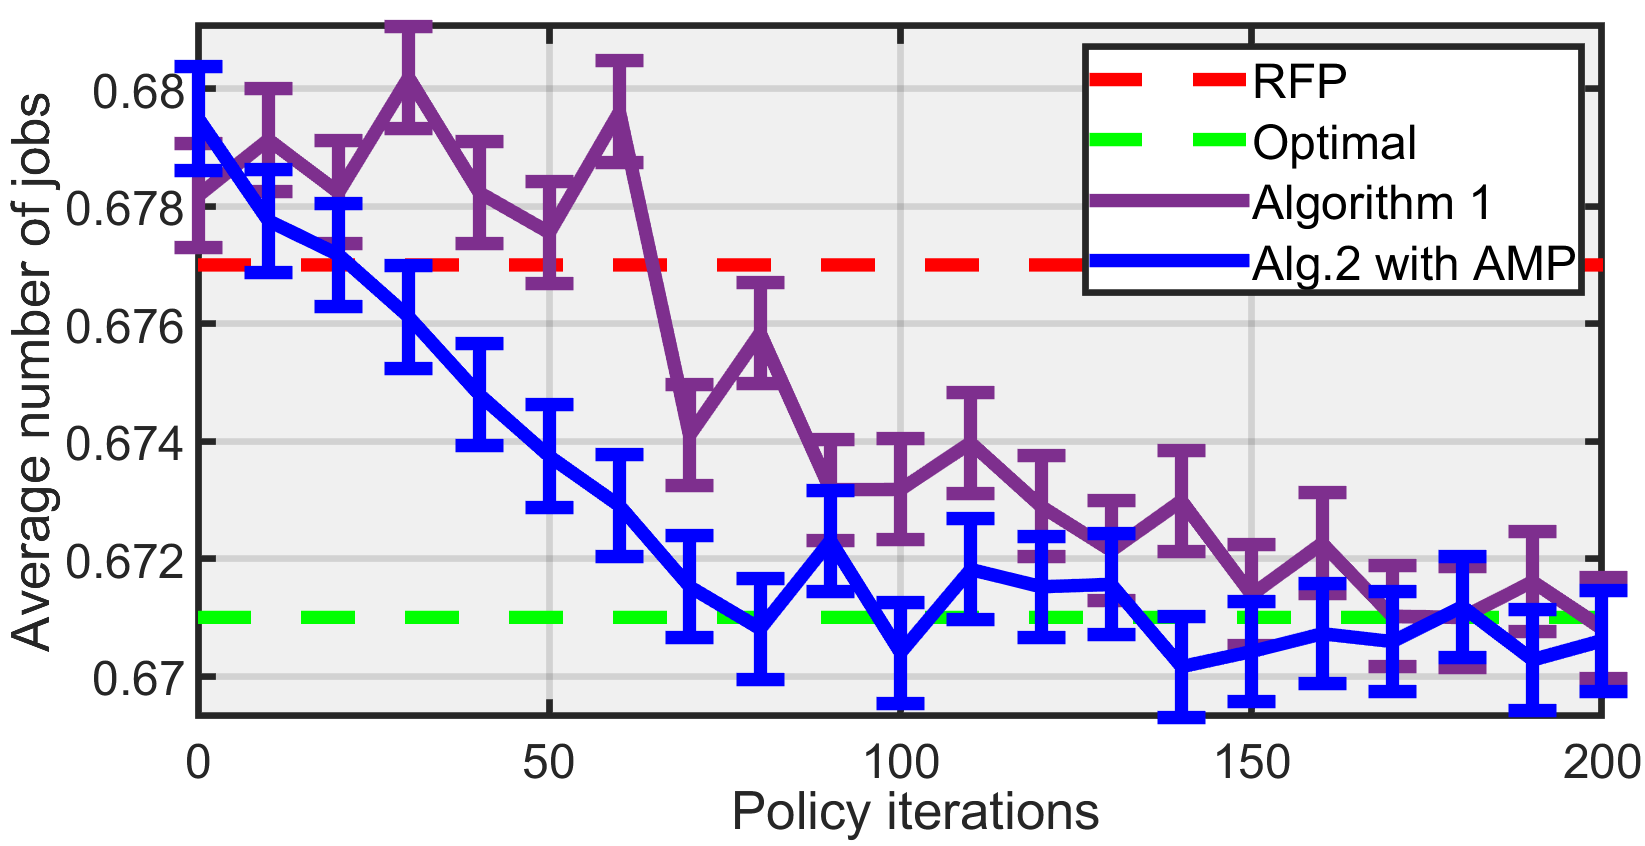
\includegraphics[ height=0.19\textwidth, width=0.35\textwidth]{ILpaper}
     }
          \subfloat[Imbalanced medium (IM) traffic \label{subfig-4:IM}]{%
       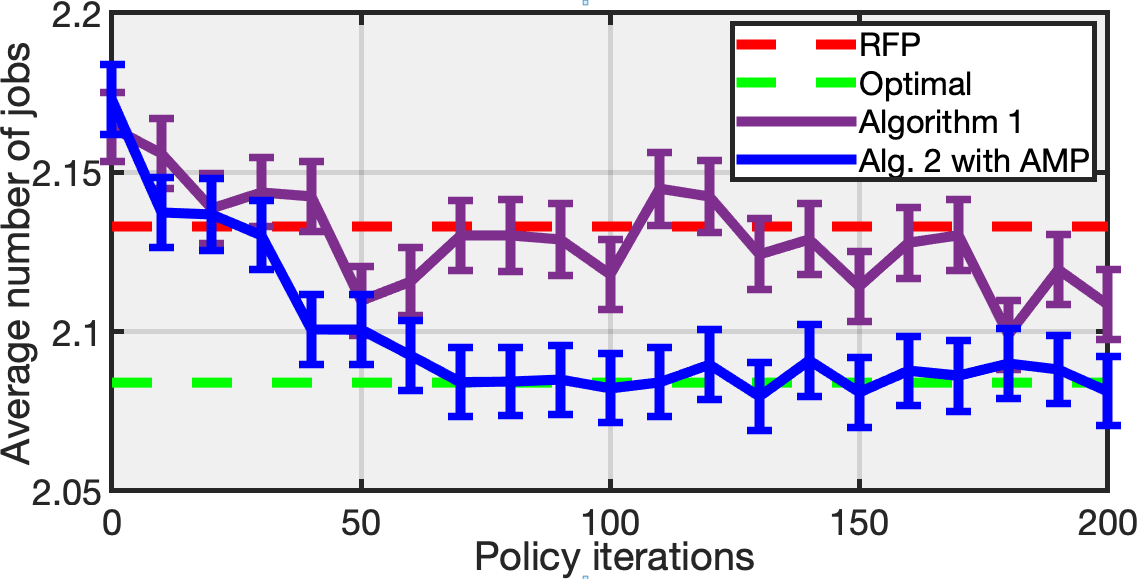
\includegraphics[ height=0.19\textwidth, width=0.35\textwidth]{IMpaper}
     }
     \subfloat[Imbalanced heavy (IH) traffic \label{subfig-2:IH}]{%
       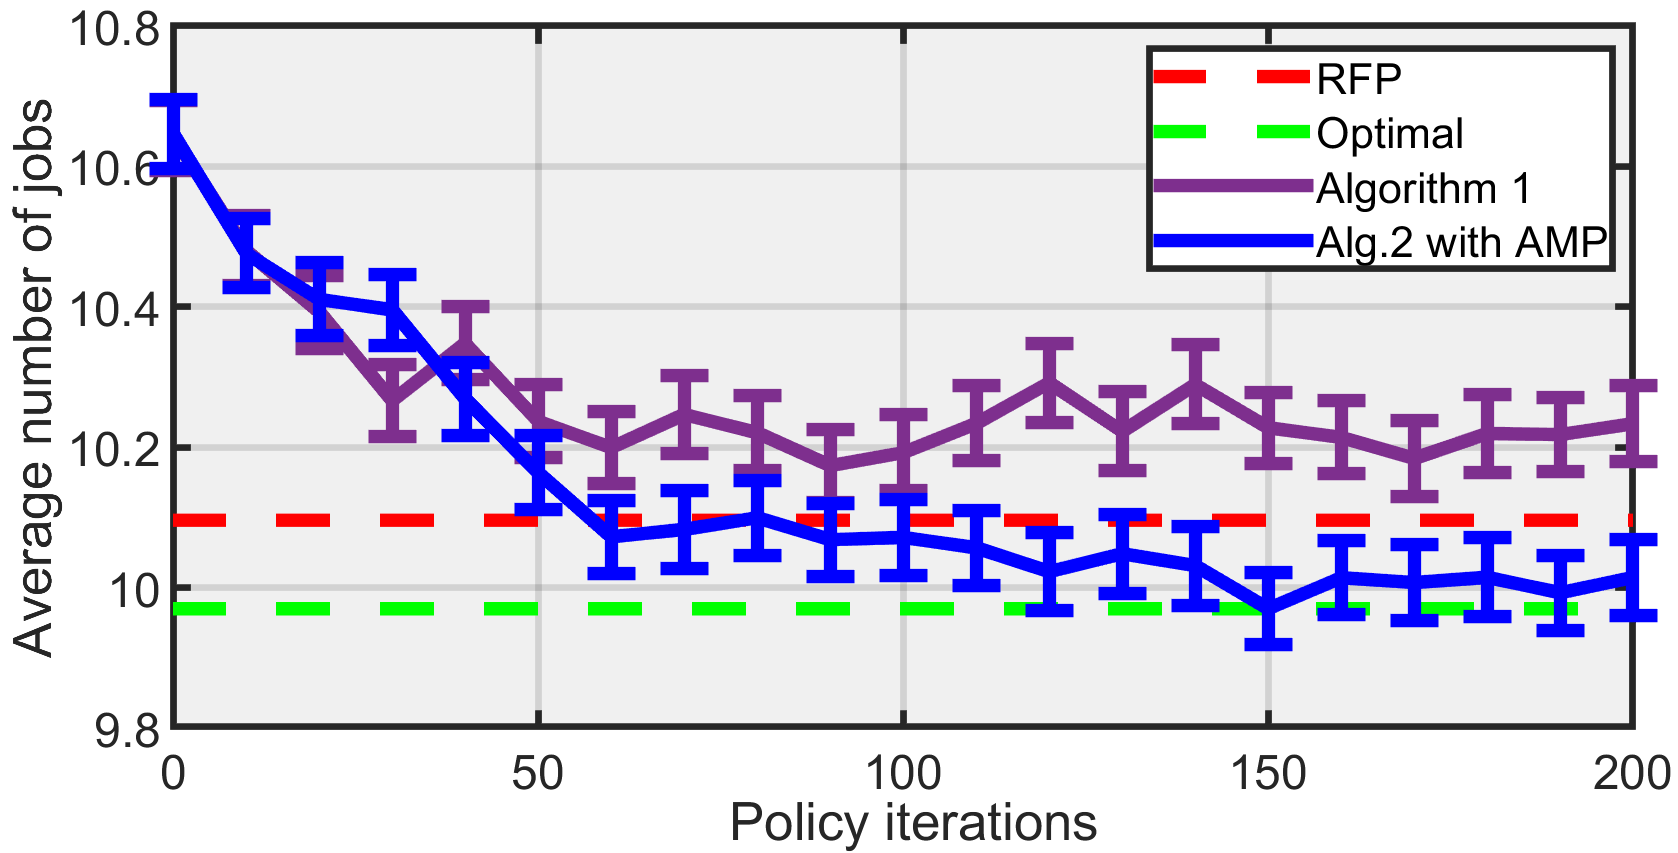
\includegraphics[ height=0.19\textwidth, width=0.35\textwidth]{IHpaper}
     }\\
           \subfloat[Balanced low (BL) traffic\label{subfig-5:BL}]{%
       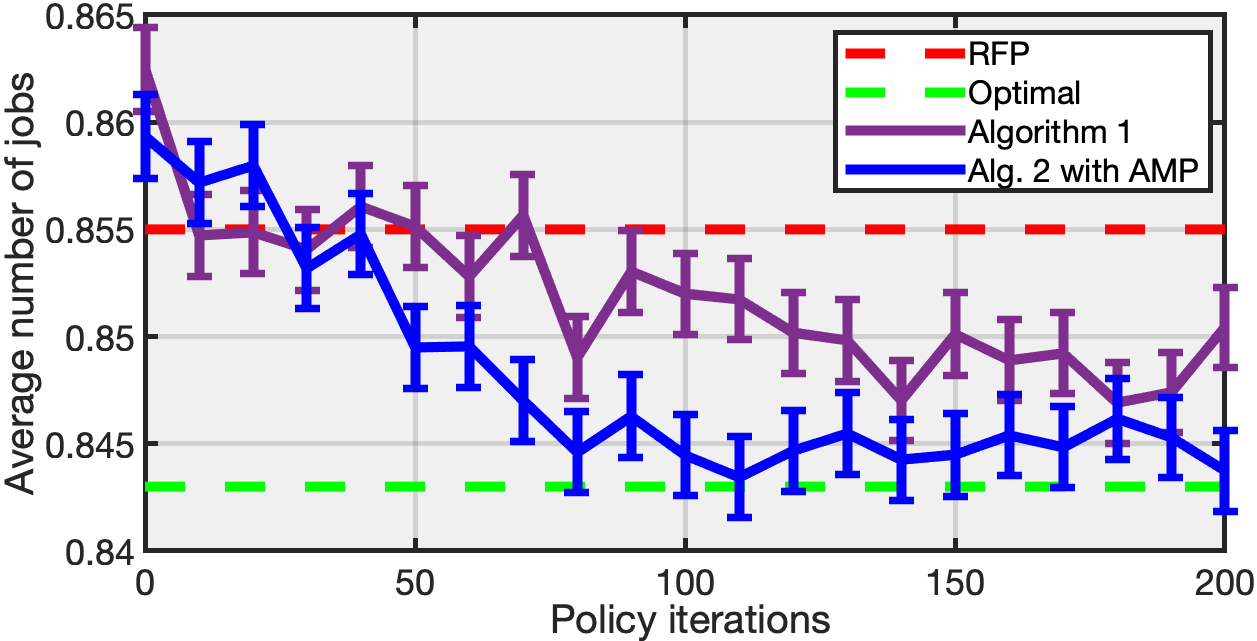
\includegraphics[  height=0.19\textwidth, width=0.35\textwidth]{BLpaper}
     } 
          \subfloat[Balanced medium (BM) traffic\label{subfig-3:BM}]{%
       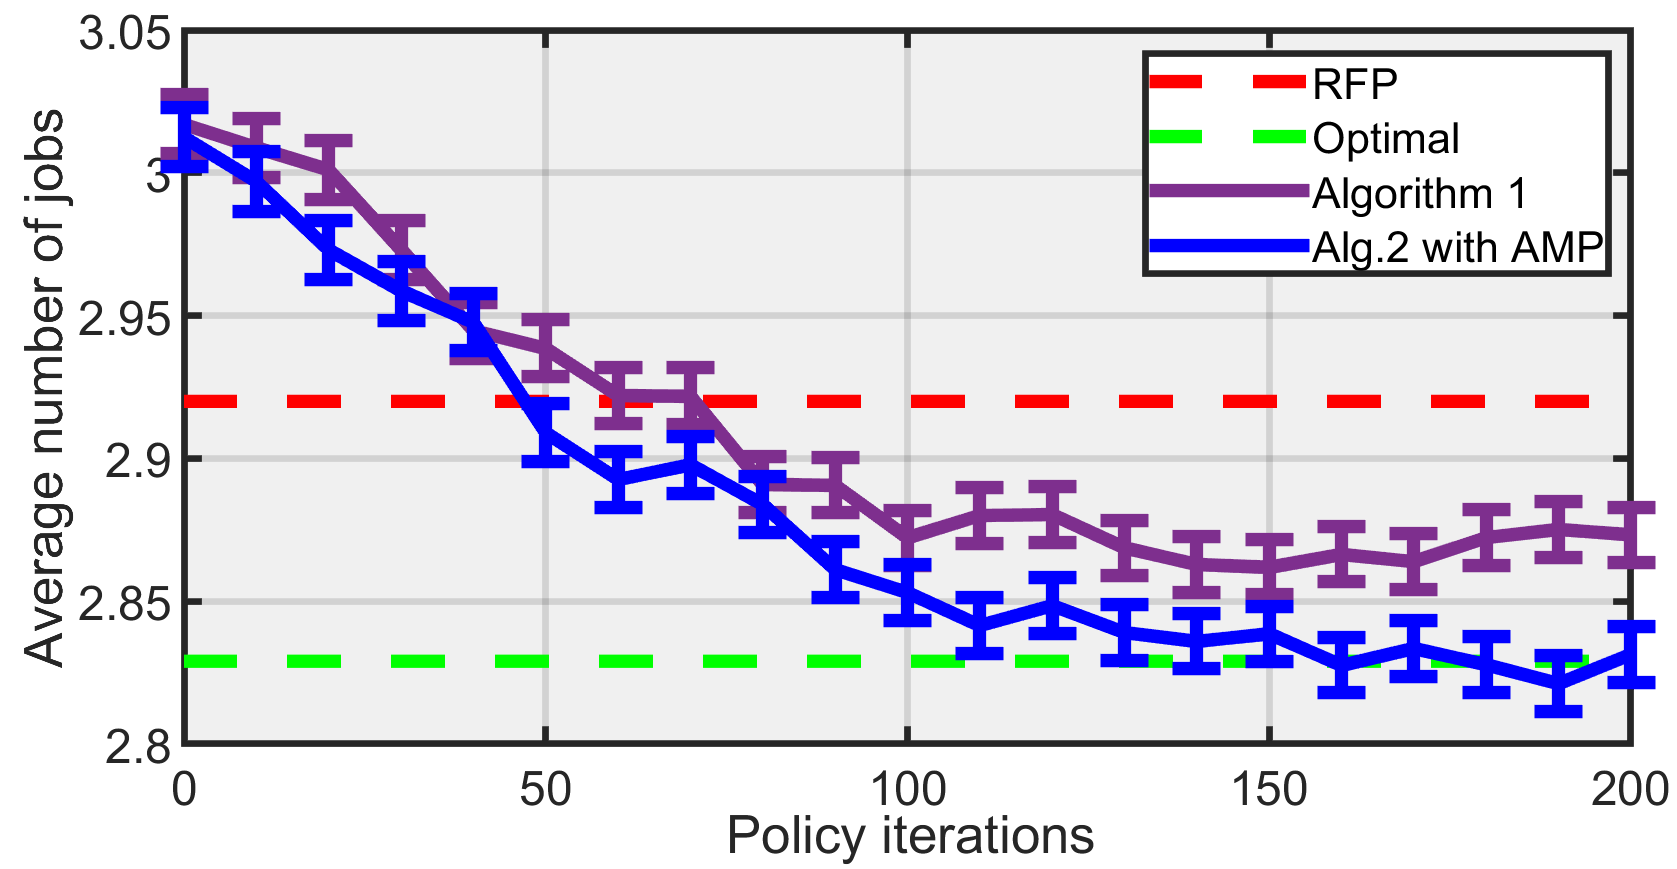
\includegraphics[  height=0.19\textwidth, width=0.35\textwidth]{BMpaper}
     } 
     \subfloat[Balanced heavy (BH) traffic\label{subfig-1:BH}]{%
       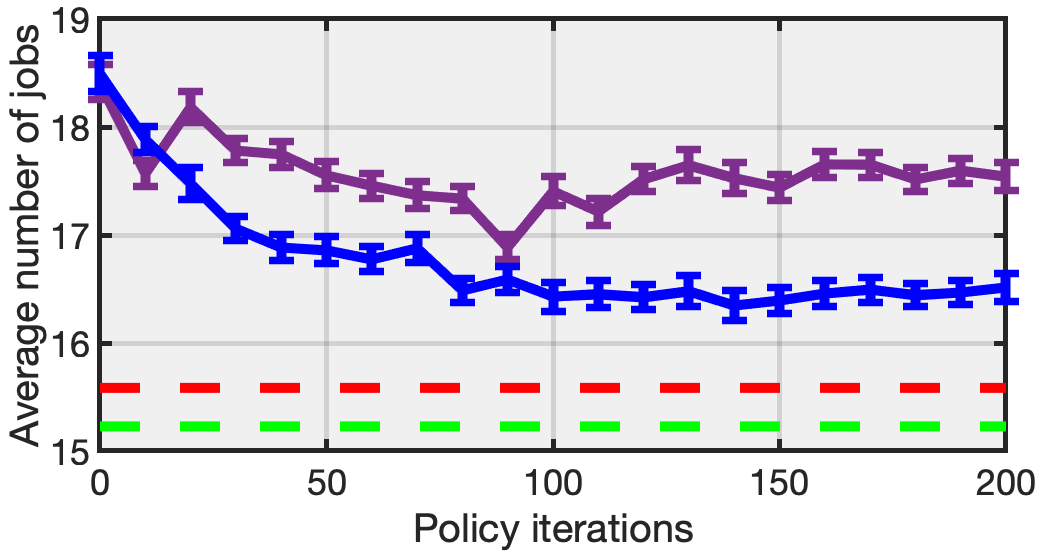
\includegraphics[ height=0.19\textwidth, width=0.35\textwidth]{BHpaper}
     }

   


   
     \caption{Comparison of learning curves from Algorithm \ref{alg1} and Algorithm \ref{alg1amp}  on the criss-cross network with different traffic regimes.  \textit{The purple (blue) solid line} shows the performance of  PPO policies obtained at the end of every 10th iterations of Algorithm \ref{alg1} (Algorithm \ref{alg1amp}, correspondingly);  \textit{red dash line} --performance of the robust fluid policy (RFP), \textit{green dash line} --performance of the optimal policy. }
     \label{fig:cc_opt}
   \end{figure}
\begin{table}[H]
\centering
\begin{tabular}{|c|c|c|c|c|c|c|c|}
  \hline
  % after \\: \hline or \cline{col1-col2} \cline{col3-col4} ...
  Load regime  & $\lambda_1$ & $\lambda_2 $ & $\mu_1$ & $\mu_2$ & $\mu_3$ & $\rho_1$ & $\rho_2$\\\hline
  I.L. & 0.3 & 0.3& 2 & 2 &1.5& 0.3&0.2\\\hline
  B.L. & 0.3 & 0.3 & 2 & 2 &1 &0.3&0.3\\\hline
  I.M. & 0.6 & 0.6  & 2 & 2 &1.5& 0.6&0.4\\\hline
  B.M. & 0.6 & 0.6  & 2 & 2 &1& 0.6&0.6\\\hline
  I.H. & 0.9 & 0.9 & 2 & 2 &1.5& 0.9&0.6\\\hline
  B.H. & 0.9 & 0.9 & 2 & 2&1&0.9&0.9 \\

  \hline


\end{tabular}
 \caption[]{Load parameters for the criss-cross network of Figure \ref{fig:cc}
 }\label{t:lp}
\end{table}



\begin{table}[H]
\centering
\begin{tabular}{|c|c|c|c|c|c|c|}
  \hline
  % after \\: \hline or \cline{col1-col2} \cline{col3-col4} ...
  Load regime  & DP (optimal) & TP & threshold & FP & RFP & PPO (Algorithm \ref{alg1amp})\\\hline
  I.L. & 0.671 & 0.678 & 0.679 & 0.678 &0.677&   0.671 \\\hline
  B.L. & 0.843 & 0.856 & 0.857 & 0.857 &0.855&  0.844 \\\hline
  I.M. & 2.084 & 2.117 & 2.129 & 2.162 &2.133& 2.084  \\\hline
  B.M. & 2.829 & 2.895 & 2.895 & 2.965 &2.920 &  2.839\\\hline
  I.H. & 9.970 & 10.13 & 10.15 & 10.398 &10.096 & 10.067 \\\hline
  B.H. & 15.228 & 15.5 & 15.5 & 18.430 &15.585&  16.513\\

  \hline


\end{tabular}

 \caption[]{Average number of jobs per unit time in the criss-cross network under different polices. The traffic regime in the network varies from imbalanced low to balanced heavy.}\label{tab:cc}%
\end{table}


Unfortunately, Algorithm \ref{alg1amp} is not robust enough and converges to a  suboptimal policy when the criss-cross network operates in balanced heavy load regime.    We run Algorithm \ref{alg2} with discount factor $\gamma=0.998$ and TD parameter $\lambda = 0.99$. Each iteration we use $Q = 50$ parallel processes to generate trajectories each with length $N=50000.$ We note that Algorithm \ref{alg2} uses approximately 10 times less samples per iteration than  Algorithm \ref{alg1amp}. Algorithm \ref{alg2} outputs policy $\pi_{\theta_{200}}$ which performance is $15.353$ jobs per unit time. See the comparison of the learning curves of Algorithm \ref{alg1amp} and Algorithm \ref{alg2} in Figure \ref{fig:cc23}.



\begin{figure}[H]
\centering%
\includegraphics[width=.6\linewidth]{cc23}
\caption[]{Comparison of learning curves from Algorithm \ref{alg1amp} and Algorithm \ref{alg2}  on the criss-cross network with balanced heavy regime. }
\label{fig:cc23}%
\end{figure}




In the next section we test the robustest of Algorithm \ref{alg2} to the size of the queuing network.  


\subsection{Extended six-class queuing network}\label{sec:ext}

In the next experiment we consider the family of extended six-class networks from \cite{Bertsimas2015} and apply Algorithm \ref{alg2} to find good control policies.

 The structure  of the  extended six-class networks is shown in Figure \ref{fig1}.
%Job classes 1 and 3 arrive externally  to the network according to a Poisson process with a rate $\lambda_1$ and $\lambda_2$, respectively. Then jobs from class 1 and class 3 follow two separate routes. Jobs from class 3 are sequentially processed in each of $L$ servers and then leave the network.  Jobs from class 1 after being processed in each server fed back into 2nd buffer associated with the first server. After the jobs of class 2 are served in each server again and then leave the system. 
The experiments have been run for the network with the following traffic parameters: $\lambda_1 = \lambda_2 = 9/140$, the service times are exponentially distributed with service rates determined  by the modulus after division the class index  by 6. That is, classes associated with server 1 are served with rates $\mu_1 = 1/8$, $\mu_2 = 1/2$, $\mu_3 = 1/4$ and classes associated with server 2 are processed with service rates $\mu_4 = 1/6$, $\mu_5 = 1/7$, $\mu_6 = 1.$  The service rates
for the odd servers $S_1, ..., S_{\lfloor L/2\rfloor+1}$ are the same as the service rates for server 1, while the service rates for the even
servers $S_2, ...., S_{\lfloor L/2 \rfloor}$ are the same as the service rates for server 2. The load is the same for each station and is equal to $\rho = 0.9$.



\begin{figure}[H]
\centering%
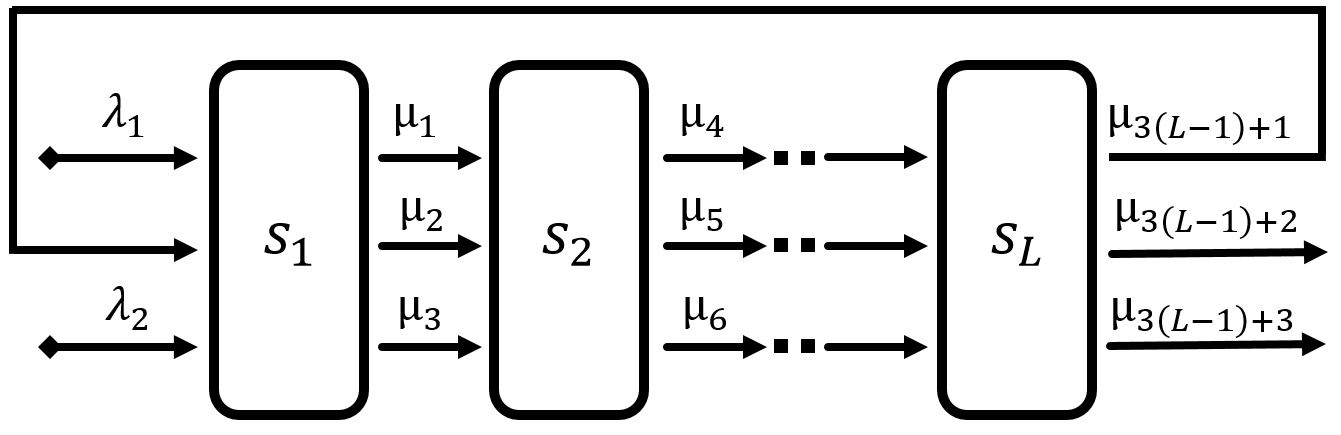
\includegraphics[width=.8\linewidth]{Paper_ext6.JPG}
\caption[]{The extended six-class network}
\label{fig1}%
\end{figure}

 Table \ref{tab6extRes} provides the performance of the PPO policy and compares it with other heuristic methods for the extended six-class queuing networks. In the experiments we change the size of the network to test the robustness of the PPO policies. The size of the networks varies from 6 to 21 classes. In all experiments we generate $Q=50$ episodes with $N=50000$ timesteps. The discount factor and TD parameter are fixed and equal to $\gamma=0.998$ and $\lambda = 0.99$ correspondingly.
In the table FP and RFP refer to fluid and robust fluid policies \cite{Bertsimas2015}.
LBFS defines the last-buffer first-serve policy, where a priority at a server is given to jobs with highest index.  FCFS refers to the first-come first-serve policy, where a priority at a server is given to jobs with the longest waiting time for service.


We have found that Xavier initialization of the policy NN yields unstable policy for   extended six-class networks. To overcome this issue we use a domain knowledge and pre-train the policy NN so that $\pi_{\theta_0}$  operates as a  \textit{proportional randomized (PR) policy} .
When the network operates under the proportional randomized policy, whenever an arrival or service completion event happens in the system,  a nonempty buffer $j$ receives a priority over other classes associated to server $s(j)$ with probability 
\begin{align}\label{eq:PRPprob}
\frac{x^j}{\sum\limits_{i\in B_{s(j)}}  x^i},
\end{align} where  $B_{s(j)}$ is a set of buffers associated to server $s(j)$ and $x = (x^1, ..., x^J)$ is a state at the time of the event.  The priority  stays fixed   until the next arrival or service completion event happens. The proportional randomized policy is similar to HLPPS (head-of-line proportional processor sharing) policy. The HLPPS policy allows processor sharing and all nonempty buffers receive  service
simultaneously. The fraction of server $s(j)$ capacity that is allocated to class $j$ is equal to (\ref{eq:PRPprob}). Therefore,  the HLPPS policy has the same expected service rate for each job class as the PR policy. 
The HLPPS policy is \textit{maximally stable} for MQNs \cite{Bramson1996} meaning that if the system is unstable under HLPPS policy there is no other policy that can stabilize it.  The PR policy is also maximally stable for open MQNs, see the proof in Section \ref{sec:PR} in Appendix.
 



We save policy parameters $\{\theta_i\}_{i=0, 10, ..., 200}$ every 10th iteration for further profound evaluation. 
The regenerative simulation is computationally intractable for large-size systems with a high load~--~time between returns to a regeneration state is very large, so that a run with many timesteps would
be required to obtain even a single regenerative cycle. For large-size networks \textit{the method of batch
means}  is recommended to estimate the performance \cite[Section 6]{Henderson1997}.  We simulate   policies $\{    \pi_{\theta_i}: i = 0, 10, ..., 200 \}$  starting from an empty state $x = (0,..,0)$ until $5\times10^6$ arrival events happened.
For each simulated trajectory the  confidence intervals are computed by splitting  on 50 sub-episodes (batches), see also \cite{Nelson1989}. Then we estimate average performance (batch mean) based on each sub-episode. Pretending that the obtained 50 estimates are i.i.d. we compute  $95\%-$confidence intervals shown on the plots.
 


\begin{figure}[H]
    \subfloat[6-classes network \label{subfig-6:IL}]{%
       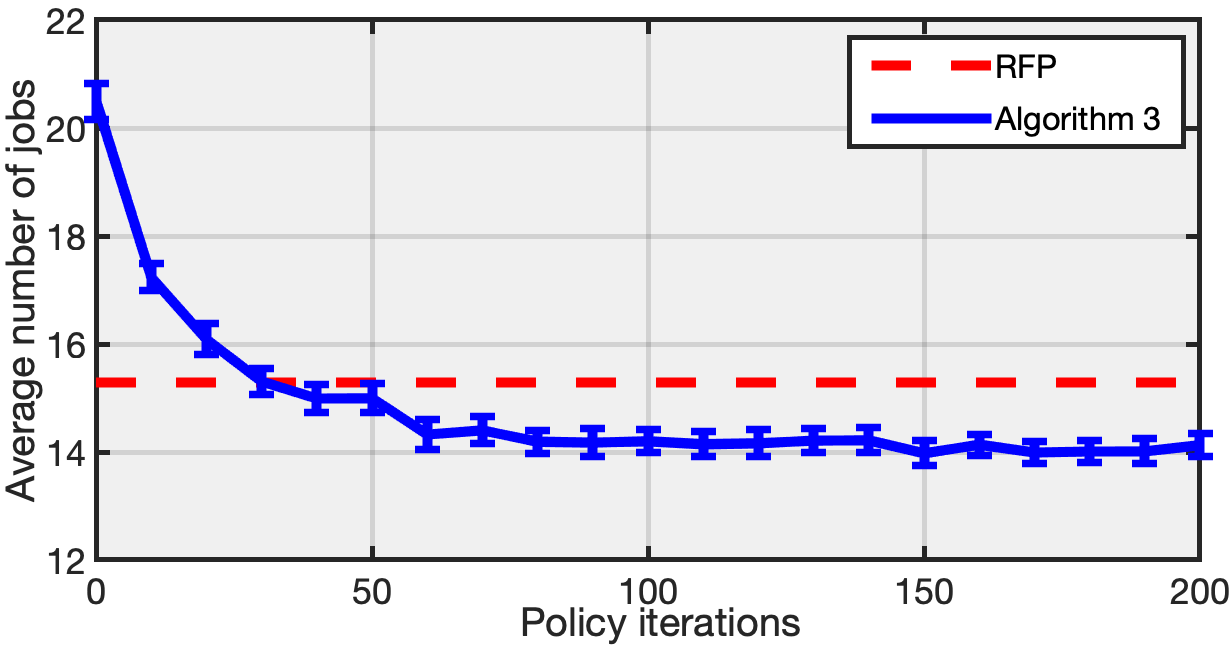
\includegraphics[height=0.2\textwidth, width=0.35\textwidth]{6classesPaper}
     }
     \subfloat[9-classes network \label{subfig-4:IM}]{%
       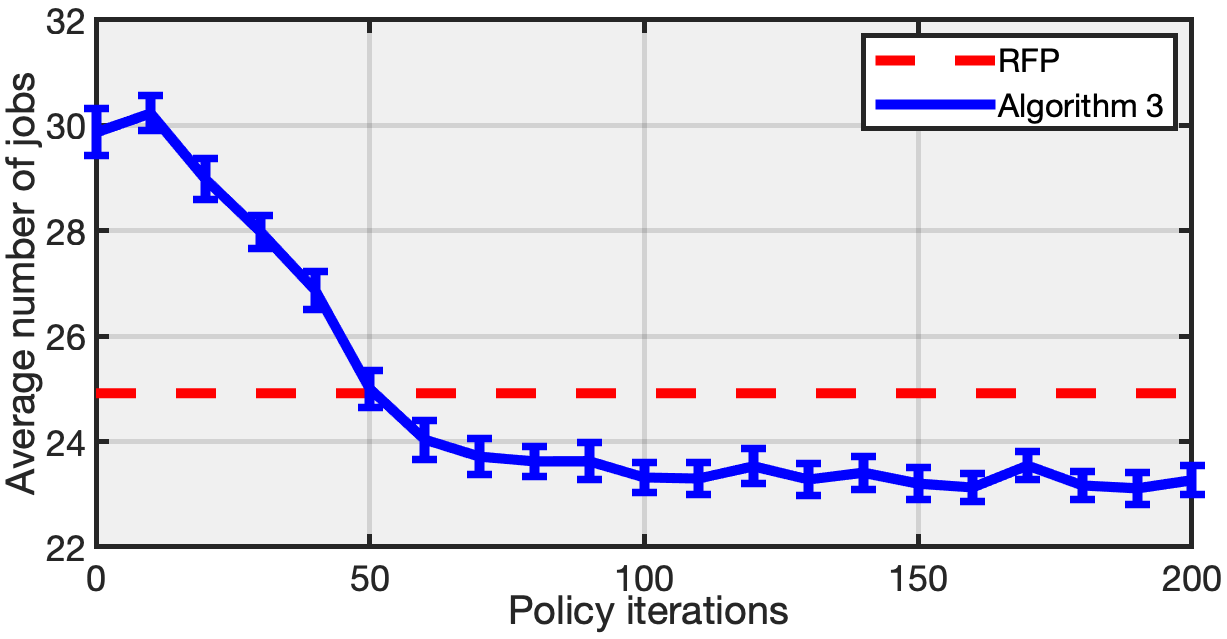
\includegraphics[height=0.2\textwidth, width=0.35\textwidth]{9classesPaper}
     }
     \subfloat[12-classes network \label{subfig-2:IH}]{%
       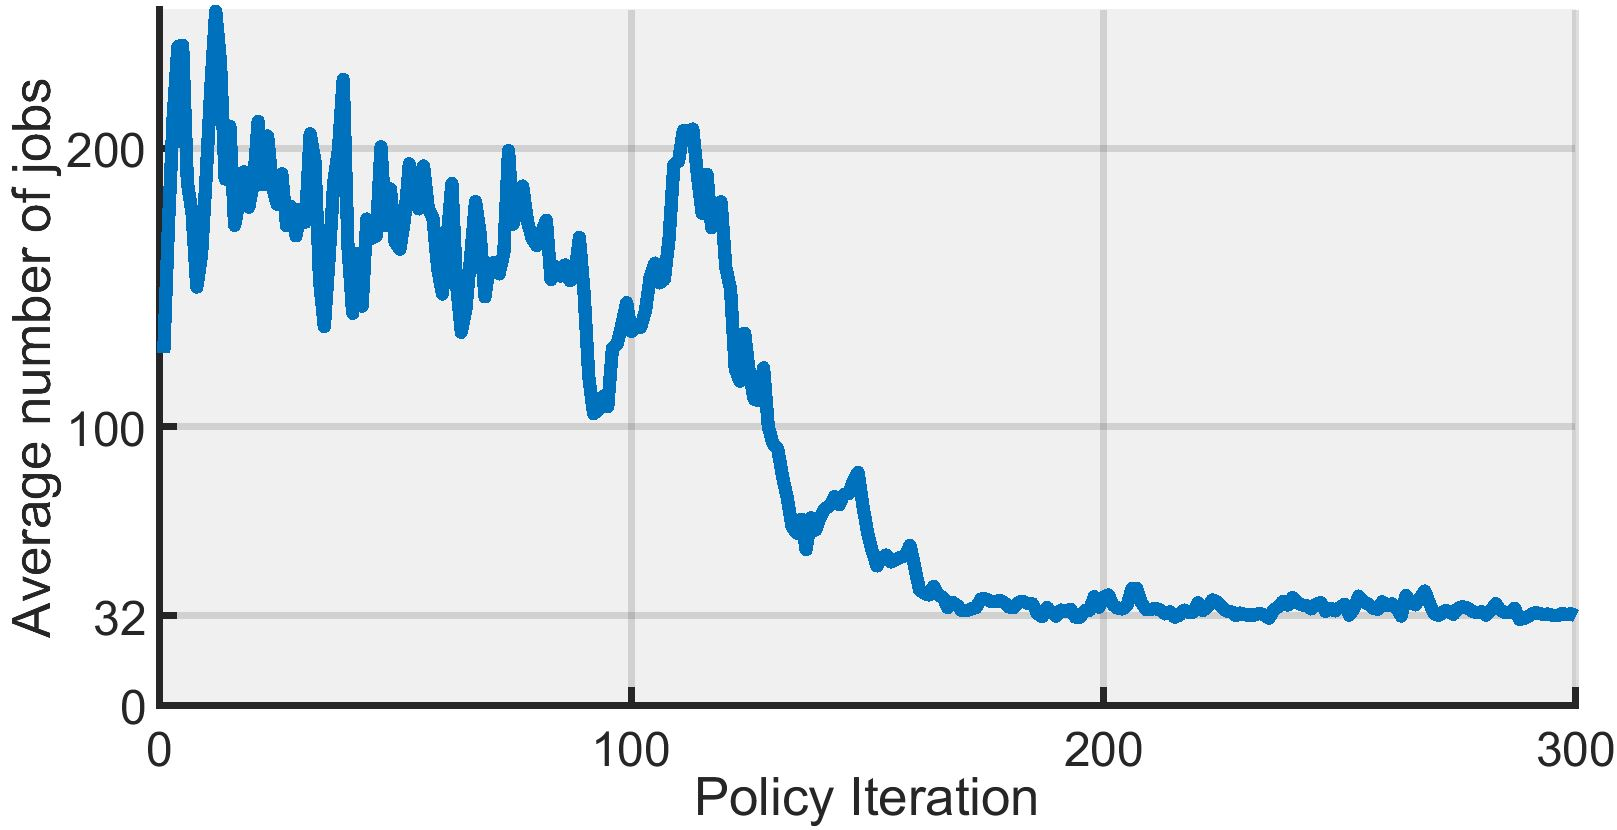
\includegraphics[height=0.2\textwidth, width=0.35\textwidth]{Paper12classes}
     }\\
 \subfloat[15-classes network\label{subfig-5:BL}]{%
       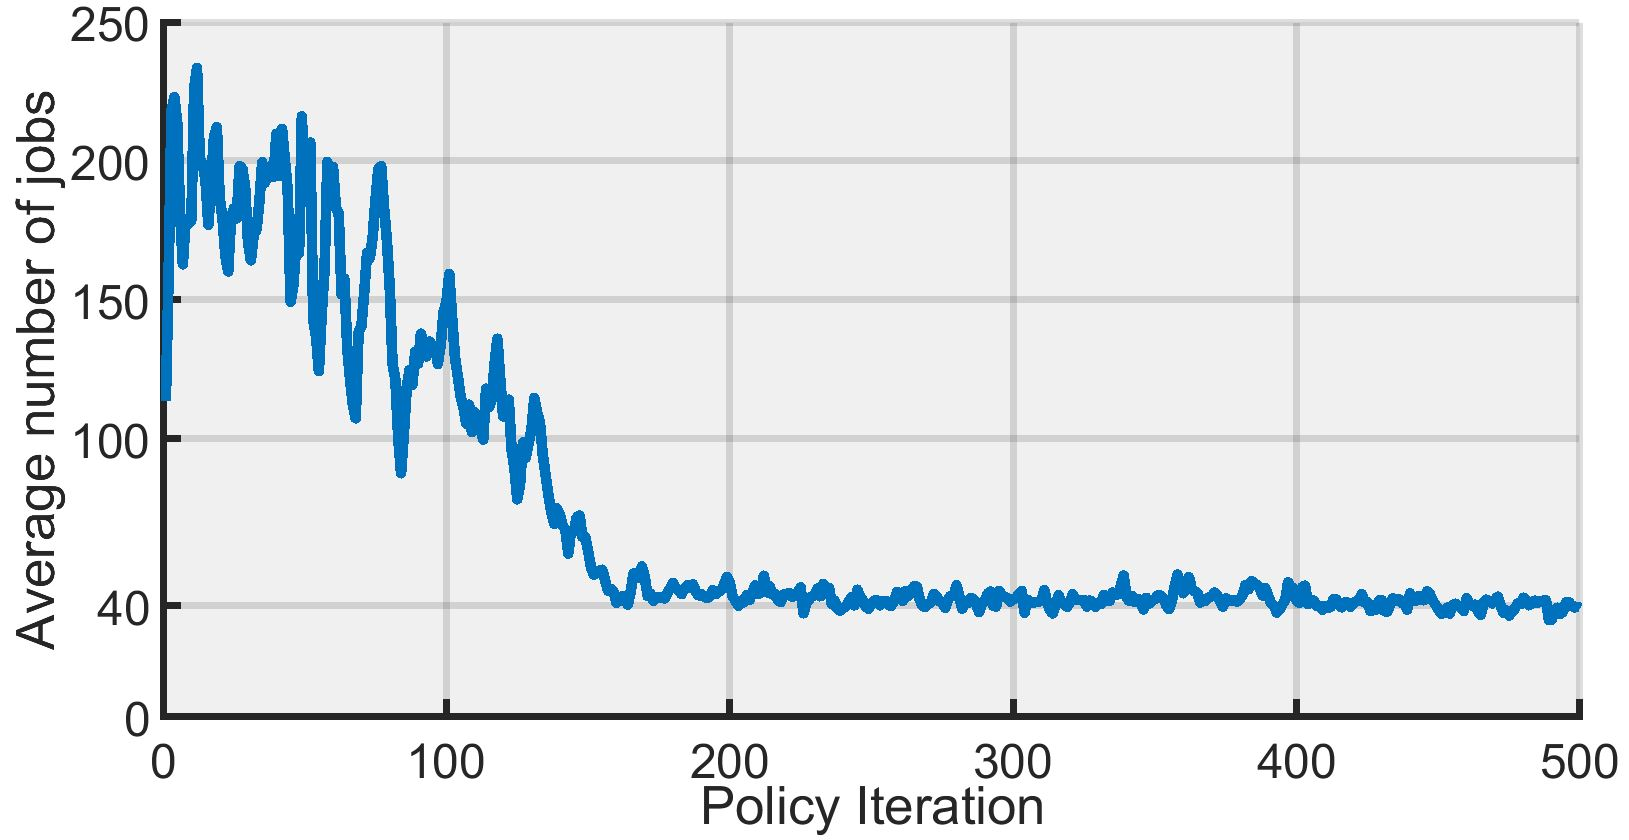
\includegraphics[ height=0.2\textwidth, width=0.35\textwidth]{Paper15classes}
     }
  \subfloat[18-classes network\label{subfig-3:BM}]{%
       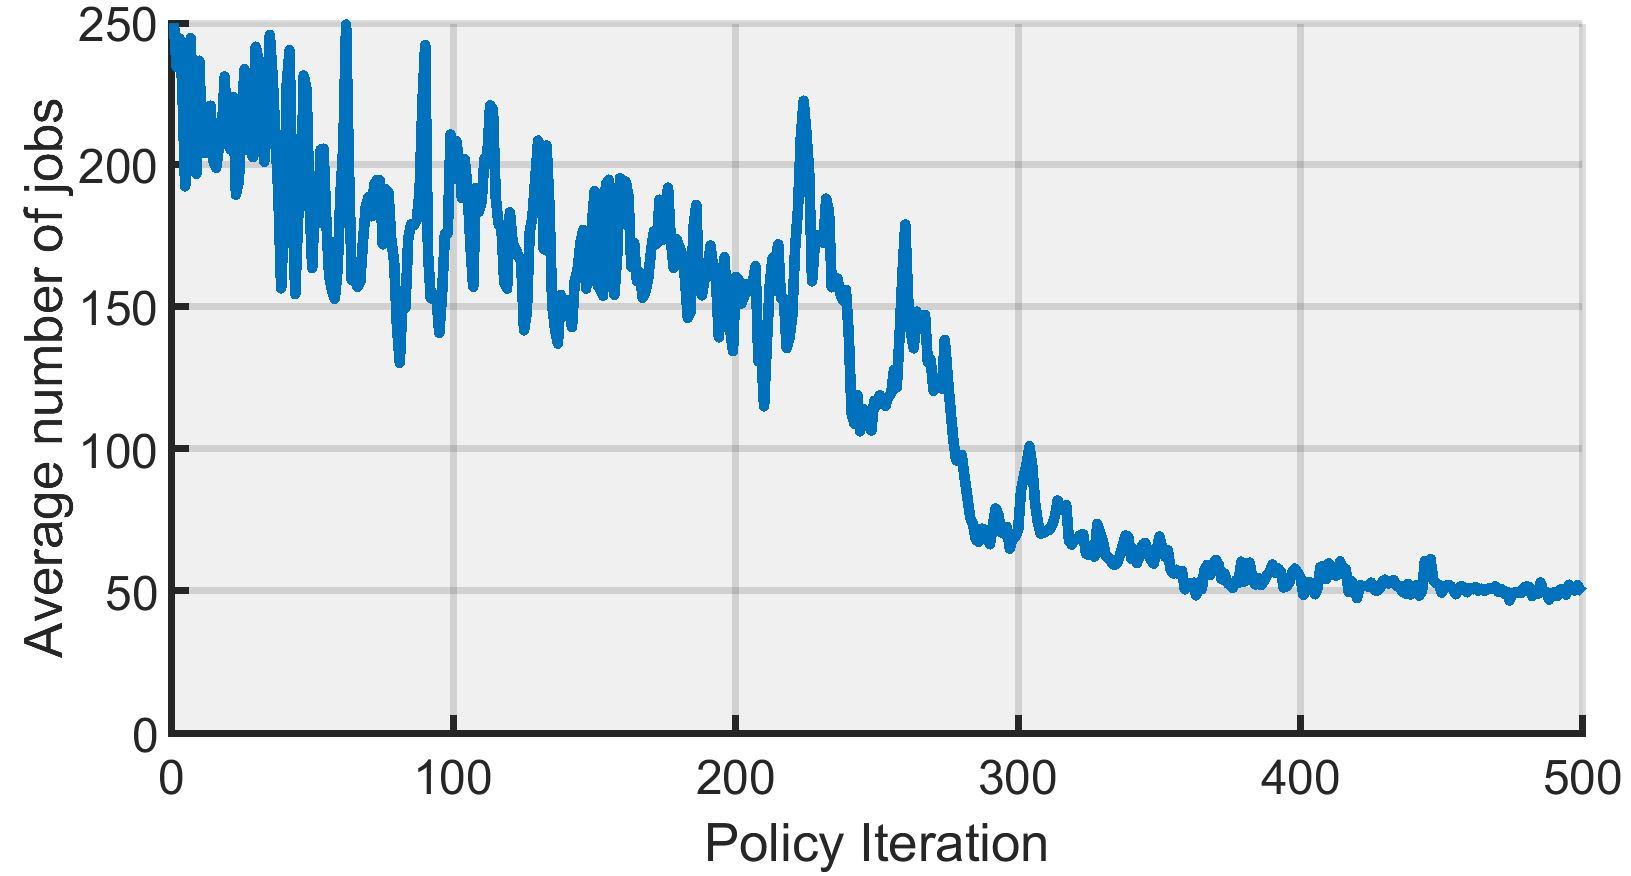
\includegraphics[ height=0.2\textwidth, width=0.35\textwidth]{Paper18classes}
     }
     \subfloat[21-classes network\label{subfig-1:BH}]{%
       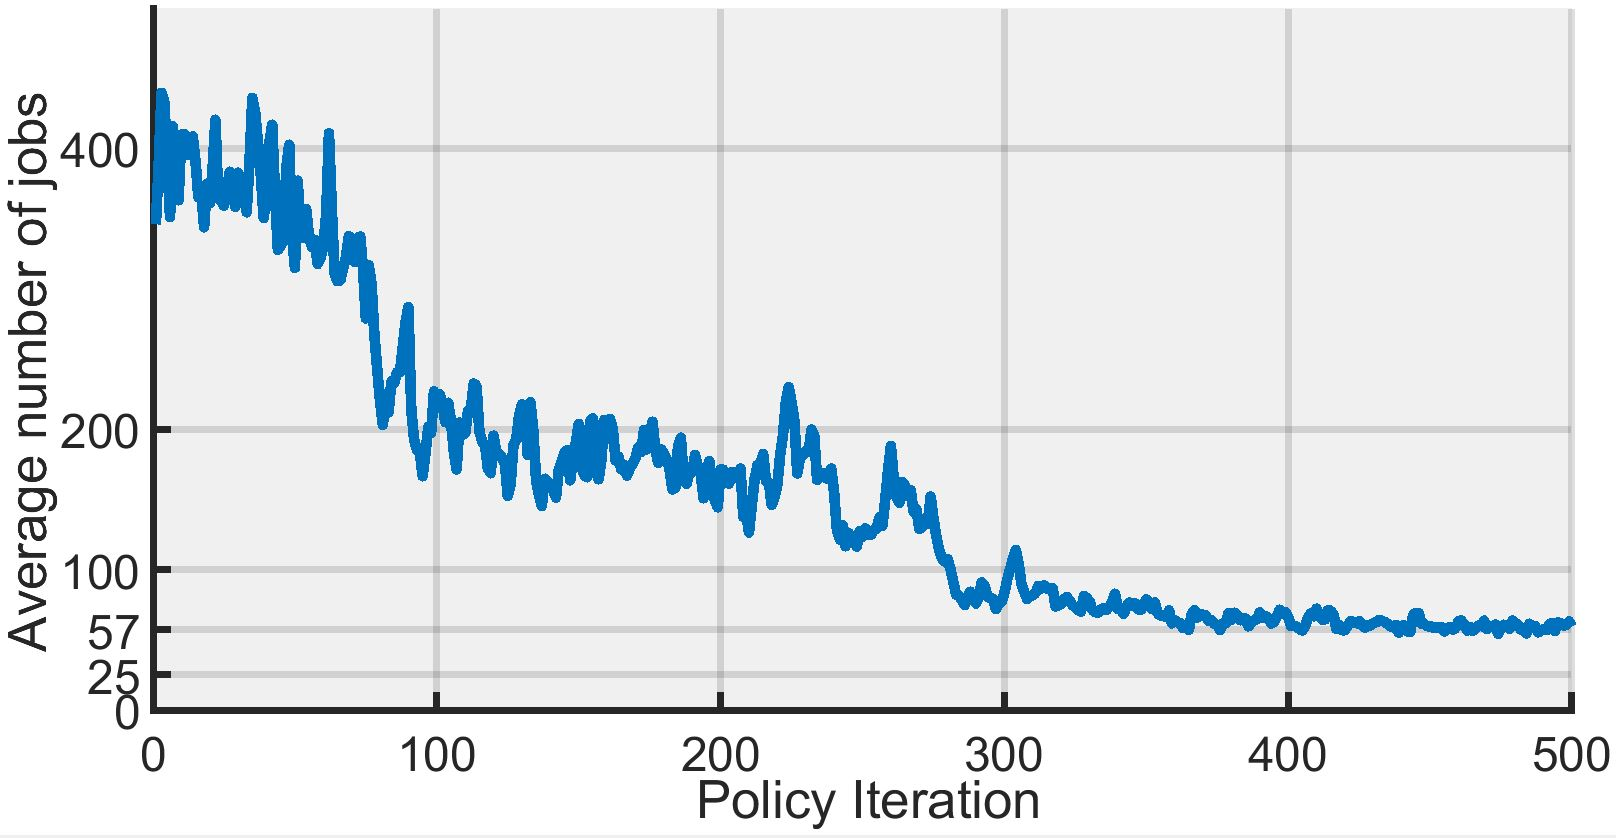
\includegraphics[ height=0.2\textwidth, width=0.35\textwidth]{Paper21classes}
     }


\caption{Learning curves  from Algorithm \ref{alg2} for the 6-class extended networks.     \textit{The blue solid line} shows the performance of  PPO policies obtained at the end of every 10th iterations of Algorithm \ref{alg2},  \textit{red dash line} --performance of the robust fluid policy (RFP).}
     \label{fig:ext_ac}
   \end{figure}

\begin{table}[H]
\centering%
\begin{tabular}{|c|c|c|c|c|c|}
  \hline
  % after \\: \hline or \cline{col1-col2} \cline{col3-col4} ...
  Num. of classes $3L$  & LBFS & FCFS & FP & RFP & PPO (Algorithm \ref{alg2})\\\hline
  6 & 15.749 & 40.173 & 15.422 & 15.286 &14.130 \\\hline
  9 & 25.257 & 71.518 & 26.140 & 24.917& 23.269 \\\hline
  12  & 34.660 & 114.860 & 38.085 & 36.857&  \\\hline
  15  & 45.110  & 157.556  & 45.962 & 43.628&  \\\hline
  18  & 55.724 & 203.418 & 56.857  & 52.980  &  \\\hline
  21  & 65.980 & 251.657 & 64.713 & 59.051 &  \\
  \hline
\end{tabular}
\caption[]{Numerical results for the extended six-class network of Figure \ref{fig1}.}\label{tab6extRes}
\end{table}

%\subsection{Extended re-entrant queuing network}
%
%
%Another network that has been proposed in \cite{Bertsimas2015} is a reentrant line with $L$ servers. Figure \ref{fig2} displays the
%topology of this queueing network. Only buffer 1 is fed by external arrivals according to a Poisson process with a rate $\lambda_1$. The network consists of $L$ services. To leave the system each job has to re-enter each server three times, thus each server processes 3 classes of jobs. The arrival rate $\lambda_1$ and all service rates of the job classes are the same as for the extended
%six-class network considered in Section \ref{sec:ext}.
%
%Learning curves showing the average number of jobs for each network are shown in Figure \ref{fig:reent_ac}.
%
%\begin{figure}[H]
%\centering%
%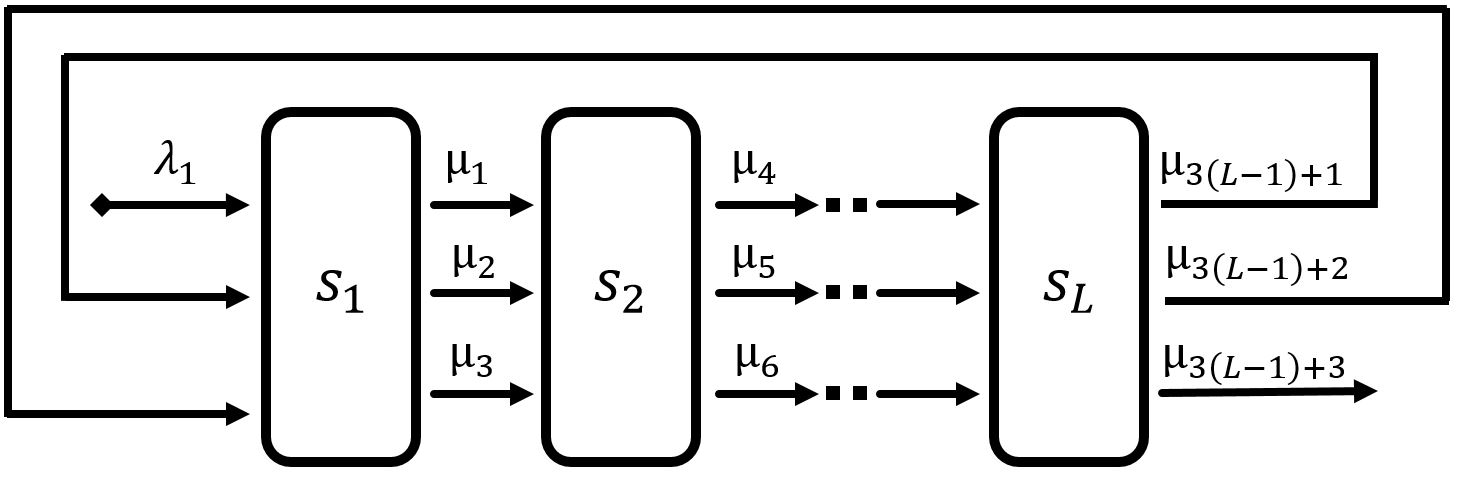
\includegraphics[width=.8\linewidth]{Paper_reentr.JPG}
%\caption[]{The extended re-entrant network}
%\label{fig2}%
%\end{figure}
%
%\begin{table}[H]
%\centering%
%\begin{tabular}{|c|c|c|c|c|c|}
%  \hline
%  % after \\: \hline or \cline{col1-col2} \cline{col3-col4} ...
%  Num. of classes $3L$  & LBFS & FCFS & FP & RFP & RL\\\hline
%  6 & 15.911 & 16.441 & 15.422 & 15.663 & 14.317\\\hline
%  9 & 30.001 & 27.154 & 25.955 & 24.015& 22.359 \\\hline
%  12  & 40.167 & 35.633 & 32.014 & 29.925& 28.856\\\hline
%  15  & 57.056  & 47.969  & 40.113 & 36.901& 36.003\\\hline
%  18  & 66.042 & 56.996 & 48.781  & 44.261  & 46.670\\\hline
%  21  & 87.136 & 71.002 & 54.711 & 48.418 & 51.512\\
%  \hline
%\end{tabular}
%\caption[]{Numerical results for the reentrant network of Figure \ref{fig2}.}\label{tabReentr}%
%\end{table}



 

\section{Conclusion}

In this study we have presented application of
deep reinforcement learning to the scheduling problem in multiclass queuing networks.




We have  proposed a theoretically-justified modification of the Proximal Policy Optimization algorithm that can be applied in the long-run average setting.  The algorithm does not require any knowledge of  topological routing structure within the network and any information about traffic intensity. Admittedly, the learning process of the RL algorithm requires intensive simulations of many different policies that may require a generative model. The proposed approach scales well and can handle networks with multiple job classes and servers if advanced enough computational infrastructure is available.






Our numerical results show that  RL policies yield almost-optimal performance for the criss-cross network and accomplish  long-run average performance within 1\% from the optimal according to Table \ref{tab:cc}. In large networks our approach leads to effective scheduling policies that outperform or perform comparable to known alternatives. In the extended six-class queuing network RL polices  outperform  the robust fluid policies on average by more than  5\%. In the extended reentrant queuing network RL polices reach comparable performance with the robust fluid policies outperforming them on the 6-, 9-, 12-, 15- classes  networks  and performing within 5\% of
RFP on 18-, 21-classes networks. Note that displayed  performance of robust fluid policy in Table \ref{tabReentr} is the performance of the best  robust fluid policy which corresponds to the best choice of policy parameters that can be different for each network. In all our experiments we have used fixed set of hyperparameters.
Nevertheless, the results for the extended re-entrant line indicate that optimization of scheduling policies for large MQNs is a challenging problem for RL methods that use discounting to approximate the policy gradient. Designing of  a stable deep RL algorithm that does not depend on the discount factor and directly optimizes long-run average performance  is an open problem.


Based on our simulation study we  provide a recommended set of hyperparameters for the algorithm in Section \ref{sec:par}  and  neural network structures for policy parametrization and approximation of the value function in Section \ref{sec:nn}. The recommended parameters of the algorithm yield stable learning process for large range of networks from the criss-cross network to the re-entrant network with 21 job classes.


Complexity of the scheduling optimization problem highly depends not only on the network topology, but on the traffic intensity. For the small criss-cross network in low traffic regime the RL policy almost coincides with the optimal policy:  up to 99\% of actions suggested  by RL policy are optimal. While   only around 85\% of actions are optimal in the heavy traffic regime, see Figure \ref{fig:cc_opt}. Therefore, the complexity of the problem can be easily adjusted.  We believe that this feature makes multiclass queuing networks potentially  good benchmark domain to test RL methods, for example cross-task generalization (transfer learning)  \cite{Nichol2018}.



In the paper we impose classical assumptions that external arrivals are Poisson and service
times are assumed to be exponentially distributed with class-dependent rates. More realistic scheduling policy optimization problem  is to design a learning algorithm for a time-dependent distribution of inter-arrival times. We hope that the current paper a small step in this direction.




\section{Appendix}





\subsection{Maximal Stability of Proportional Randomized Policy}\label{sec:PR}

In this section we consider proportional randomized policy. 

Associated with each decision is a random proportional vector for $\gamma = (\gamma_1, ..., \gamma_J)\geq 0$ and satisfies $\sum\limits_{i\in B_l} \gamma_i =1$ and $\max\limits_{i\in B_l}\gamma_i =1$ for each server $l$.



For a job class $i\in B_l$ the fraction of server $k$ the probability to get full service capacity is proportional to population size at the decision epoch. 
\begin{align*}
\Prob(\gamma_i = 1) = \frac{x_i}{\sum\limits_{j\in B_l} x_j}
\end{align*}


Non-negative $J-$vector $\beta$ of class-level service rates going forward from a decision time $t$, 

\begin{align}
\beta_i(t) = 
\begin{cases}
\gamma_i \text{ if }z_i(t)>0,\\
0, \text{ otherwise}
\end{cases}
\end{align}

Define a non-decreaseing $J-$dimentional process $T  = \{T(t), ~t\geq 0\}$ whose $j$th component $T_j(t)$ represents the cumulative amount of service effort devoted to jth class over the time interval $(0, t].$ It can be expressed mathematically:
\begin{align}
T_j(t):=\int\limits_0^t \beta_i(u)du,\quad \text{ for each class } j\text{ and } t\geq 0.
\end{align}


In the fluid model, for all $t\geq 0$ we have


\begin{align}\label{eq:fluid}
\dot Z(t) = \lambda - (I-P')M\beta(t)\\
C\beta(t)\leq e\\
Z(t)\geq 0\\
\beta(t)\geq 0
\end{align}


The functions $Z_i(t)$ and $T_i(t)$ are absolutely continuous, and thus, differentiable almost everywhere. The equations \ref{eq:fluid} hold for all times $t$ at which $Z_i(t)$ and $T_i(t)$ are differentiable.


For a job class $i\in B_l$ the fraction of server define ``an expected'' service allocation given queue lengths at time $t$ is
   \begin{align}
   \hat \beta_i(t) := 
   \begin{cases} 
   \frac{z_i(t)}{\sum\limits_{j\in B_l} z_j(t)} \text{ if } \sum\limits_{j\in B_l} z_j(t)>0\\
   0, \text{ otherwise}
   \end{cases}
   \end{align} 

  
  
  
  For each initial state $z\in \Z_+^L$ and $t > 0 $, 
  
  \begin{align}
  \xi_i^z(t) := \int \limits_{0}^t ( \beta_i^z(u)  - \hat \beta_i^z(u)) du
  \end{align} 

Let us explicitly write $Z^z(t, \omega)$ for a particular sample path $\omega$ of $Z^z(t).$



\begin{lemma}
Let $\{z^r: r\geq 1\}\subset \Z_+^r$ be a sequence of initial states satisfying $|z^r|\geq r^2$ for each $r\geq 1$, then with probability 1:

\begin{align}
\lim\limits_{r\rightarrow \infty} \frac{\xi^{z^r}(|z^r, \omega|) }{|z^r|}=0
\end{align}

\begin{proof}
By Chebyshev's inequality:

\begin{align}
\Prob\left\{ \omega: \frac{|\xi_i^{z^r}(|z^r, \omega|)|}{|z^r|} >\epsilon\right\}\leq \frac{\E\left[ \xi_i^{z^r} (|z^r|) \right]^2}{\epsilon^2|z^r|^2}
\end{align}


Let $\{\tau_k\}_{k=0}^K$ are the decision epochs before time and $\tau_{K+1} = |z^r|$, where $\tau_0=0$ then 

\begin{align}
&\E\left[ \xi_i^{z^r} (|z^r|) \right]^2 = \E \left[\int\limits_0^{|z^r|} (\beta(u) - \hat\beta(u))  du  \right]^2 =  \E \left[\sum\limits_{k=0}^{K}\int\limits_{\tau_k}^{\tau_{k+1}} (\beta(u) - \hat\beta(u))  du \right   ]^2=\\
&\E\sum\limits_{k=0}^{K}   \left ( \int\limits_{\tau_k}^{\tau_{k+1}} (\beta(u) - \hat\beta(u))  du \right)^2    + 2 \sum\limits_{k<k'}^{K} \E  \left ( \int\limits_{\tau_k}^{\tau_{k+1}} (\beta(u) - \hat\beta(u))  du \right)\left ( \int\limits_{\tau_k'}^{\tau_{k'+1}} (\beta(u) - \hat\beta(u))  du \right)=\\
&  \E \sum\limits_{k=0}^{K} \left ( \int\limits_{\tau_k}^{\tau_{k+1}} (\beta(u) - \hat\beta(u))  du \right)^2  \leq \E\sum\limits_{k=0}^{K}    \left ( \int\limits_{\tau_k}^{\tau_{k+1}} 1  du \right)^2\leq \E\sum\limits_{\tau'\in \text{arrivals}}(\tau'_{k+1} - \tau'_{k})^2\leq O(|z^r|) 
\end{align}
where the second inequality follows from the fact that 

\begin{align}
&\E \sum\limits_{k<k'}^{K} \E  \left ( \int\limits_{\tau_k}^{\tau_{k+1}} (\beta(u) - \hat\beta(u))  du \right)\left ( \int\limits_{\tau_k'}^{\tau_{k'+1}} (\beta(u) - \hat\beta(u))  du \right)=\\
&\E\left[ \sum\limits_{k<k'}^{K} \E  \left ( \int\limits_{\tau_k}^{\tau_{k+1}} (\beta(u) - \hat\beta(u))  du \right) \E \left[\left ( \int\limits_{\tau_k'}^{\tau_{k'+1}} (\beta(u) - \hat\beta(u))  du \right)| Z(\tau_k')\right]\right]=0
\end{align}

Hence $\Prob\left\{ \omega: \frac{|\xi_i^{z^r}(|z^r, \omega|)|}{|z^r|} >\epsilon\right\}\leq \frac{1}{\epsilon^2 r^2}$ the lemma follows from the Borel-Cantelli lemma. 

\end{proof}

\end{lemma}





\begin{theorem}
Consider a multiclass queueing network operating under the random proportional policy. Let $\{z^r:r\geq 1\}\subset \Z^r_+$ be a sequence of initial states satisfying $|z^r|\geq r^2$ for each $r\geq 1$, and let $\Omega$ be as in Lemma \ref{lem:conv}. For each $\omega\in \Omega_1 \sup \Omega_2$, all fluid limits $(\hat D, \hat T, \hat Z)$ satisfying the following: for each packet class $i\in I$

\begin{align}
\frac{d}{dt}\hat T_i(t) = \frac{\hat Z_i(t)}{\sum\limits_{j\in B_l} \hat Z_j(t)}\text{ when }
\sum\limits_{j\in B_l} \hat Z_j(t)>0.
\end{align}



\begin{proof}

Assume that $\{z^r:r\geq 1\}\subset \Z_+^r$ is a sequence of initial states satisfying $|z^r|\geq r^2.$ Fix an $\omega \in \Omega_1\sup \Omega_2$. Let $(\hat D(\cdot), \hat T(\cdot), \hat Z(\cdot))$ be a fluid limit path. Fix a buffer $i$ and $t>0$, and let $l\in L$ be an associated server to buffer $i$. Assume that $\hat Z_i(t)>0.$ By the continuity of $\hat Z_i(\cdot)$, there exists a $\delta\in (0, t)$ s.t. 

\begin{align}
\epsilon:=\min\limits_{u\in [t-\delta, t+\delta]}\hat Z_i(u)>0. 
\end{align}

Thus, there exists $Z_i^{z_n}(u)\geq |z_n|\epsilon/2\geq 1$ for $u\in (|z_n|(t-\delta), |z_n|(t+\delta))$ and $n\geq L_0.$

Next,


\begin{align}
T_i^{z_r}(|z_r|u_2) - T_i^{z_r}(|z_r|u_1) = \int \limits_{|z_r|u_1}^{|z_r|u_2}  \beta_i^z(u) du= \int \limits_{|z_r|u_1}^{|z_r|u_2}  \hat \beta_i^z(u) du+ \xi_i^{z_r} (|z_r|u_2) -  \xi_i^{z_r}(|z_r|u_1).
\end{align}



We have proved that $\lim\limits_{r\rightarrow \infty} \frac{1}{||z^r||}\left[ \xi_i^{z_r} (|z_r|u_2) -  \xi_i^{z_r}(|z_r|u_1) \right]= 0$.


Hence

\begin{align}
\hat T_i^{z_n}(u_2) - \hat T_i^{z_n}(u_1) = \int\limits_{u_1}^{u_2} \hat \beta (\hat Z^{z_r}(u))du 
\end{align}
\end{proof}
\end{theorem}


 



\subsection{AMP estimator for discounted advantage function}\label{sec:AMPforDisc}


In order to derive the corresponding AMP estimator for the discounted advantage function we define an infinite-horizon discounted state-action value function
\begin{align*}
Q^{(\gamma)}_\eta(x, a) : =  \E \left[ \sum\limits_{t=0}^\infty \gamma^{t }  g(x_t)  \Big| x_0 = x\right] \text{ for each }(x, a)\in \X\times \A,
\end{align*}
where $x=x_0$, action $a = a_0$ is taken at time $k=0$ and actions according to policy $\pi_\eta$ are taken at each time $k\geq 1.$



 Assume that an approximation $ \tilde V$ of the infinite-horizon discounted value function $V_{\eta}$ is available. Define the following martingale sequence $(M_{\eta}^{(n)}:n\geq 0), ~\eta\in \Theta$ where
\begin{align}\label{eq:mart}
M_{\eta}^{(n)}(x):=\sum\limits_{k=1}^n \gamma ^{k}[ \tilde V (x_k) - \sum\limits_{x'\in X} P_{\eta}(x'|x_{k-1})  \tilde V(x')  ],
\end{align}         
where   $x = x_0$ and $x_k$ is a state of the Markov chain $P_\eta$ at time $k$.

By \cite[Propositions 3, 7]{Henderson2002} if $\mu_{\theta}(V_{ \theta})<\infty$ then $M_{\theta}^{(n)}\rightarrow M^{{\infty}}$ a.s. and $\E M_{\theta}^{(\infty)} =0$.  The fact that  $\mu_{\eta}^TV_\eta<\infty$ follows from  $\mu_{\eta}^T V_\eta = \frac{\mu^T_\eta g}{1-\gamma}$, see \cite[Section 10.4.]{Sutton2018}.
        

The method does not add any bias subtracting $M_\infty$ from $\hat Q^{(\gamma)}_\eta$. We get the AMP  estimator of the discounted state-action value function:
\begin{align*} 
\hat Q^{ AMP( \tilde V), (\gamma)}_{\eta}(x ) & :=  \hat Q_\eta^{(\gamma)}(x, a ) - M_{\eta}^{(\infty)}(x)\\
&=  g(x_0 ) +  \gamma \sum\limits_{x'\in X} P_{\eta}(x'|x_0)  \tilde V(x') +    \sum\limits_{k=1}^\infty\gamma^k \left(g(x_k ) +  \gamma \sum\limits_{x'\in X} P_{\eta}(x'|x_k)  \tilde V(x')   -   \tilde V(x_k )  \right)
\end{align*}
where $x=x_0$, action $a = a_0$ is taken at time $k=0$ and actions according to policy $\pi_\eta$ are taken at each time $k\geq 1.$

We take $\tilde V$ as a baseline for the state-action value function and  get the AMP  estimator of the discounted advantage function:  
\begin{align*} 
\hat A^{AMP(\tilde V), (\gamma)} (x_k, a_k) :=  \sum\limits_{k=0}^\infty\gamma^k \left(g(x_k ) +  \gamma \sum\limits_{x'\in X} P_{\eta}(x'|x_k)  \tilde V(x')   -   \tilde V(x_k )  \right)  
\end{align*}


\subsection{Proofs}\label{sec:proofs}

 \begin{lemma}\label{lem:norms}

For any vector $\nu$ on $\X$ we consider the following norms w.r.t.  vector $\V:\X\rightarrow [1, \infty]$:
\begin{align*}
||\nu||_{1, \V}:=\sum\limits_{x\in \X} |\nu(x)|\V(x)\\
||\nu||_{\infty, \V} := \sup\limits_{x\in \X} \frac{|\nu(x)|}{\V(x)} 
\end{align*}

We also consider the following $\V$-weighted operator norm for a matrix $T\in \M_{\X\times \X}$:
\begin{align*}
||T||_\V:=\sup\limits_{x\in \X} \frac{1}{\V(x)} \sum\limits_{y\in \X} |T(x, y)|\V(y).
\end{align*}

The operator norm $||\cdot||_\V$ is equivalent to the norm  induced from norm $||\cdot||_{1, \V}$ and  to the norm induced from norm $||\cdot||_{\infty, \V}$, i.e. for any matrix  $T\in \M_{\X\times \X}$:

\begin{align*}
||T||_\V = \sup\limits_{\nu:||\nu||_{1, \V}=1} ||\nu T ||_{1, \V} = \sup\limits_{h:||h||_{\infty,\V} = 1} || Th ||_{\infty, \V}
\end{align*}


\begin{proof}

First, consider $\sup\limits_{h:||h||_{1, \V} = 1} || Th ||_{1, \V}$ norm. On the one hand, 
\begin{align*}
 \sup\limits_{\nu:||\nu||_{1, \V}=1} ||\nu T ||_{1, \V} \geq \sum\limits_{y\in X} \V(y) \left| \sum\limits_{x\in X} \frac{T(x, y)}{\V(x)}   \right| = ||T||_\V
\end{align*}

On the other hand, 
\begin{align*}
 \sup\limits_{\nu:||\nu||_{1, \V}=1} ||\nu T ||_{1, \V}  &= \sup\limits_{\nu:||\nu||_{1, \V}=1}   \sum\limits_{y\in X}   \sum\limits_{x\in X} |T(x, y) \nu(x)| \V(y) \\
& \leq  \sup\limits_{\nu:||\nu||_{1, \V}=1}   \sum\limits_{y\in X}   \sum\limits_{x\in X}  \frac{1}{\V(x)}~|T(x, y)| ~ \V(y) ~ |\nu(x)|~ \V(x)\\
& \leq \sup\limits_{x\in X} \sum\limits_{y\in X}   \frac{1}{\V(x)} |T(x, y)|  \V(y) \sup\limits_{\nu:||\nu||_{1, \V}=1}  \sum\limits_{x\in X} |\nu(x)| \V(x)\\
& = ||T||_\V
\end{align*}

Similar for $\sup\limits_{h:||h||_{\infty, \V} = 1} || Th ||_{\infty, \V}$ norm:
\begin{align*}
 \sup\limits_{h:||h||_{\infty, \V} = 1} || Th ||_{\infty, \V}  \geq ||T\V ||_{\infty, V} = ||T||_\V
\end{align*}
and 

\begin{align*}
 \sup\limits_{h:||h||_{\infty, \V} = 1} || Th ||_{\infty, \V}   &= \sup\limits_{h:||h||_{\infty, \V}=1}   \sup\limits_{x \in X}  \frac{1}{\V(x)}  \sum\limits_{y\in X} |T(x, y) h(y)|  \\
& \leq  \sup\limits_{h:||h||_{\infty, \V}=1}   \sup\limits_{x \in X}  \frac{1}{\V(x)}  \sum\limits_{y\in X} |T(x, y)| \V(y)  \frac{|h(y)|}{\V(y)}\\
 &\leq   \sup\limits_{x\in X}  \frac{1}{\V(x)}  \sum\limits_{y\in X} |T(x, y)| \V(y)     \sup\limits_{h:||h||_{\infty, \V}=1} \sup\limits_{y\in \X}\frac{|h(y)|}{\V(y)}\\
 &=||T||_\V
\end{align*}

\end{proof}
\end{lemma}

\st*
\begin{proof}

We denote $U_{\theta, \eta}: = [P_{\theta} - P_{\eta}] Z_{\eta}$  and define matrix $H_{\theta, \eta}$ as
\begin{align}\label{eq:H}
H_{\theta,\eta} := \sum\limits_{k=0}^\infty U^k_{\theta, \eta}
\end{align}

Convergence in $\V$-weighted norm in definition (\ref{eq:H}) follows  from assumption $||U_{\theta, \eta}||_\V<1$.

The goal of this proof is to show that the Markov chain  has a unique stationary distribution $\mu_{\theta}$ s.t. \begin{align}\label{eq:mu12}
\mu_{\theta}^T = \mu_{\eta}^T H_{\theta,\eta}\end{align} 


Let $\nu^T :=  \mu_{\eta}^T H_{\theta,\eta}$.  We use $e = (1, 1, ...,1,..)^T$ to denote a unit vector.   

 We first verify that $\nu^T e = \sum\limits_{x\in \X} \nu(x)=1.$ We note that $(I - P_\eta +\Pi_\eta)e = e-e+e = e$, hence $Z_{\eta} e = e.$ Then 
 \begin{align*}
 \nu ^T e = \mu_{\eta}^T H_{\theta,\eta} e = \mu_\eta^T \sum\limits_{k=0}^\infty  [P_{\theta} - P_{\eta}]^k Z_{\eta}^k e = \mu_\eta^T I e = 1.
 \end{align*} 
 
 
 Next we verify that $\nu^T P_{\theta} = \nu^T.$
 Suppose that $P_{\theta}- P_{\eta} + U_{\theta, \eta}  P_{\eta} = U_{\theta, \eta}$ then we get
 
 \begin{align*}
\nu^T P_{\theta} &=\mu_{\eta}^T \sum\limits_{k=0}^\infty U_{\theta, \eta}^k P_{\theta} \\
&=   \mu_{\eta}^T \sum\limits_{k=0}^\infty U_{\theta, \eta}^k P_{\theta}- \mu_{\eta}^T \sum\limits_{k=0}^\infty U_{\theta, \eta}^k P_{\eta} + \mu_{\eta}^T \sum\limits_{k=0}^\infty U_{\theta, \eta}^{k} P_{\eta}\\
& =  \mu_{\eta}^T +   \mu_{\eta}^T \sum\limits_{k=0}^\infty U_{\theta, \eta}^k P_{\theta}- \mu_{\eta}^T \sum\limits_{k=0}^\infty U_{\theta, \eta}^k P_{\eta} + \mu_{\eta}^T \sum\limits_{k=0}^\infty U_{\theta, \eta}^{k+1} P_{\eta} \\
& =  \mu_{\eta} ^T+ \mu_{\eta}^T \sum\limits_{k=0}^\infty U_{\theta, \eta}^k [P_{\theta}- P_{\eta} + U_{\theta, \eta}  P_{\eta}]\\
& =\mu_{\eta}^T + \mu_{\eta}^T \sum\limits_{k=0}^\infty U_{\theta, \eta}^{k+1}\\
& =\mu_{\eta}^T \sum\limits_{k=0}^\infty U_{\theta, \eta}^{k}\\
& = \nu^T
 \end{align*} 
 
 It is left  to show 
   \begin{align}\label{eq:Pfinite}
   P_{\theta}- P_{\eta} + U_{\theta, \eta}  P_{\eta} = U_{\theta, \eta}.
    \end{align} 
   Indeed,   
      \begin{equation*} 
\begin{aligned}[c]
   P_{\theta}- P_{\eta} + U_{\theta, \eta}  P_{\eta}& = P_{\theta}- P_{\eta} +  [P_{\theta} - P_{\eta}] Z_{\eta}   P_{\eta}& \quad &          \Big([P_{\theta} - P_{\eta}] Z_{\eta} \Big)  P_{\eta} =     [P_{\theta} - P_{\eta}] \Big(Z_{\eta}  P_{\eta} \Big)    \text{ by \cite[Corollary 1.9]{Kemeny1976}}\\
   & =  (P_{\theta}- P_{\eta} )(I + Z_{\eta}   P_{\eta} )\\
   & = (P_{\theta}- P_{\eta} )(I -\Pi_{\eta} + Z_{\eta}   P_{\eta} ) & \quad &   (P_{\theta}- P_{\eta}) \Pi_{\eta}=0  \\
   & =   (P_{\theta}- P_{\eta} )(I - Z_{\eta}  \Pi_{\eta} + Z_{\eta}   P_{\eta} )    & \quad &      Z_{\eta}  \Pi_{\eta} = \Pi_{\eta}  \\
   & =  (P_{\theta}- P_{\eta} ) Z_{\eta} & \quad &  I = Z_{\eta}(I + \Pi_\eta - P_\eta) = Z_\eta + Z_\eta \Pi_\eta - Z_\eta P_{\eta} \\
   & = U_{\theta, \eta}
\end{aligned}
 \end{equation*}
   
 
The uniqueness of the stationary distribution follows from the fact that the Markov chain with transition matrix $P_{\theta}$ is irreducible.


\end{proof}




\main*
\begin{proof}
We denote $U_{\theta, \eta}: = [P_{\theta} - P_{\eta}] Z_{\eta}$. Under assumption $||U_{\theta, \eta}||_\V<1$  operator $H_{\theta, \eta}:=\sum\limits_{k=0}^{\infty}U^k_{\theta, \eta} $ is well-defined and $||H_{\theta, \eta}||_\V\leq \frac{1}{1 - D_{\theta, \eta}}$, see the proof of Lemma \ref{lem:st}.


The stationary distribution of the Markov chain with transition matrix $P_\theta$ can be represented as  $\mu_\theta^T = \mu_{\eta}^T H_{\theta, \eta}$, see equation (\ref{eq:mu12}). We get $\mu_\theta^T\V = \mu_\eta H_{\theta, \eta}\V<\infty.$ 

By \cite[Theorem 14.1.4]{Meyn2009} the fundamental matrix for the Markov chain with transition matrix $P_\theta$ 
\begin{align*}
Z_\theta = \sum\limits_{k=0}^\infty (P_\theta - \Pi_\theta)^k
\end{align*}
is well-defined in $\V$-weighted norm sense. 

Consider matrix $T \in \M_{\X\times\X}$ that has to satisfy two properties: 1) $||T||_V<\infty$ and 2) $(I-P_\theta +\Pi_\theta)T =T(I-P_\theta +\Pi_\theta) = I$. We note that if such a matrix exists its uniqueness follows from associativity of matrices with finite $\V-$weighted norm. It is easy to see that $Z_\theta$ satisfies both requirements.

The following equation has been proved for the finite state space in \cite[Theorem 2]{Schweitzer1968}, see also \cite{Glynn1996}:  
\begin{align}\label{eq:Z}
Z_\theta = Z_{\eta}H_{\theta, \eta} - \Pi_{\eta} H_{\theta, \eta}[P_\theta - P_{\eta}]Z^2_{\eta}H_{\theta, \eta}.
\end{align}  
We have shown that all matrices in (\ref{eq:Z}) are well-defined and one can directly follow the proof of \cite[Theorem 2]{Schweitzer1968} to generalize the statement for the countable state space.


The long-run average costs difference is equal to
\begin{equation*}
\begin{aligned}[c]
\mu_\theta^Tg - \mu_\eta^Tg &= \mu_\theta^Tg+ \mu_{\theta}( [P_\theta-I]h_{\eta} )- \eta_{\eta} & \quad &\mu_{\theta}( [P_\theta-I]f) =0  \\
&=\mu_{\theta}(g + P_\theta h_{\eta}  - h_{\eta} ) -\eta_{\eta}\\
&=\mu_{\eta}(g  - \mu_\eta^Tg  e + P_\theta h_{\eta}  -h_{\eta}) + (\mu_{\theta} - \mu_{\eta})(g+P_\theta h_{\eta}  - h_{\eta} ) & \quad & \pm \mu_{\eta}(g  + P_\theta h_{\eta}  -h_{\eta})\\
& = \mu_{\eta}(g  -(\mu_\eta^Tg)  e + P_\theta h_{\eta}  -h_{\eta}) + (\mu_{\theta} - \mu_{\eta})(g - (\mu_\eta^Tg ) e +P_\theta h_{\eta}  - h_{\eta} ) &  \quad &(\mu_{\theta} - \mu_{\eta})(\mu_\eta^Tg  e)=0
\end{aligned}
 \end{equation*}
 
For any vector $\nu$ on $\X$ we define  the following norm w.r.t.  vector $\V:\X\rightarrow [1, \infty]$:  
 \begin{align*}
||\nu||_{1, \V}:=\sum\limits_{x\in \X} |\nu(x)|\V(x)
\end{align*}
We note that for any vectors $\nu_1, \nu_2$ on $\X$ and matrix $T\in \M_{\X\times \X}$ the following inequality holds, see Lemma \ref{lem:norms}:
\begin{align*}
||\nu_1^T T \nu_2||_\V\leq ||\nu_1||_{1, \V}||T||_\V|| \nu_2 ||_{\infty, \V}
\end{align*}
 
Now we are ready to bound the last term:
\begin{equation*} 
\begin{aligned}[c]
 |(\mu_{\theta} - \mu_{\eta}) & (g - \eta_{\eta}e +P_\theta h_{\eta}  - h_{\eta} )|\\
 &\leq ||\mu_{\theta} - \mu_{\eta}  ||_{1, \V}~ ||g - (\mu_{\eta}^T g)e +P_\theta h_{\eta}  - h_{\eta} ||_{\infty, \V}  \\
 &=||\mu_{\theta} - \mu_{\eta}  ||_{1, \V}~||[ P_\theta - P_{\eta}] h_{\eta}  ||_{\infty, \V}& \quad & g - (\mu_{\eta}^T g)e +P_{\eta} h_{\eta}  - h_{\eta} \equiv 0 \\
 &\leq ||\mu_{\theta} - \mu_{\eta}  ||_{1, \V}~|| [P_\theta - P_{\eta}] Z_{\eta} (g - (\mu_{\eta}^T g)e)  ||_{\infty, \V} & \quad &h_{\eta} = Z_{\eta} (g - \mu_\eta^Tg e) \\
 &\leq  ||\mu_{\theta} - \mu_{\eta}  ||_{1, \V}~|| [P_\theta - P_{\eta}] Z_{\eta}||_\V~ || (g - \mu_\eta^Tg e)  ||_{\infty, \V}\\
 &=  D_{\theta, \eta}  ||\mu_{\theta} - \mu_{\eta}  ||_{1, \V}~|| (g -(\mu_{\eta}^T g) e)  ||_{\infty, \V}   & \quad &   ||  [P_{\theta} - P_{\eta}] Z_{\eta}||_\V =  D_{\theta, \eta} \\
 &  =  D_{\theta, \eta} || \mu_{\eta}[P_{\eta} - P_{\theta}] Z_\theta ||_{1, \V}~|| (g - \mu_\eta^Tg e)  ||_{\infty, \V}   & \quad &    \mu_{\eta} - \mu_{\theta}  =  \mu_{\eta}[P_{\eta} - P_{\theta}] Z_\theta~\text{from }(\ref{eq:mu12}) \\
\end{aligned}
 \end{equation*}
     
   
     
    The only term that depends on $\theta$ is $|| \mu_{\eta}[P_{\eta} - P_{\theta}] Z_\theta ||_{1, V}$ which we bound next:
      
      
    \begin{equation*} 
\begin{aligned}[c]
     || \mu_{\eta}[P_{\eta} - P_{\theta}] Z_\theta||_{1, \V} &=  || \mu_{\eta}[P_{\eta} - P_{\theta}] Z_{\eta} (I+\Pi_\eta - P_\eta) Z_\theta||_{1, \V}& \quad &  Z_{\eta} (I+\Pi_\eta - P_\eta) = I\\
     & \leq \mu_{\eta}(\V)  D_{\theta, \eta}  || (I+\Pi_\eta - P_\eta) Z_{\theta} ||_\V  & \quad & ||  [P_{\eta} - P_{\theta}] Z_{\eta} ||_\V = D_{\theta, \eta}  \\
     & = \mu_{\eta}(\V)  D_{\theta, \eta}  ||  H_{\eta, \theta} - (I+\Pi_\eta - P_\eta) \Pi_{\eta} H_{\eta, \theta}[P_\theta - P_{\eta}]Z^2_{\eta}H_{\eta, \theta}   ||_\V    & \quad &  \text{by (\ref{eq:Z})}\\
     &  \leq   \mu_{\eta}(\V)  D_{\theta, \eta}  \left( \frac{1}{1- D_{\theta, \eta} } + ||I+\Pi_\eta - P_\eta||_\V \mu_{\eta}(\V) \frac{ D_{\theta, \eta} }{(1- D_{\theta, \eta} )^2} ||Z_{\eta}||_\V  \right)
\end{aligned}
 \end{equation*}
     
     
     
\end{proof}







\policies*

\begin{proof}

    \begin{equation*} 
\begin{aligned}[c]
     ||  [P_{\theta} - P_{\eta}] Z_{\eta}||_\V&\leq  ||  P_{\theta} - P_{\eta} ||_\V||Z_{\eta}||_\V\\
     & = ||Z_{\eta}||_\V\sup\limits_{x\in X}\frac{1}{\V(x)} \sum\limits_{y\in X} |P_{\theta} - P_{\eta}|_{x, y} \V(y)\\
     & = ||Z_{\eta}||_\V\sup\limits_{x\in X}\frac{1}{\V(x)} \sum\limits_{y\in X} | \sum\limits_{a\in A} P(y|x, a)\pi_\theta(a|x) - \sum\limits_{a\in A} P(y|x, a)\pi_{\eta}(a|x)| \V(y)\\
          & \leq ||Z_{\eta}||_\V\sup\limits_{x\in X}\frac{1}{\V(x)} \sum\limits_{y\in X} \sum\limits_{a\in A} P(y|x, a) | \pi_\theta(a|x) -  \pi_{\eta}(a|x)| \V(y)\\
          & =||Z_{\eta}||_\V\sup\limits_{x\in X}    \sum\limits_{a\in A} | \pi_\theta(a|x) -  \pi_{\eta}(a|x)|    \frac{\sum\limits_{y\in X} P(y|x, a) \V(y) }{\V(x)} \\
          &= ||Z_{\eta}||_\V\sup\limits_{x\in X}    \sum\limits_{a\in A} \Big| \frac{\pi_\theta(a|x)}{ \pi_{\eta}(a|x)} - 1\Big|   G(x, a)
\end{aligned}
 \end{equation*}
\end{proof}





\begin{lemma}\label{lem:disc}

Consider a $\V$-uniformly ergodic Markov chain  with transition matrix $P$. Let $h $ be the fundamental solution of the Poisson's equation (\ref{eq:Poisson}) for the chain  with one-step cost function $g(\cdot)$,  s.t. $|g(x)|<\V(x)$ for each $x\in \X.$ Let $J_{  \gamma}: = \sum\limits_{t=0}^\infty \gamma^{t+1} P ^t (g -  \mu^T g ) $ be the corresponding infinite-horizon discounted relative value function.

 Then for some constants $R<\infty$ and $r<1$ we have
\begin{align*}
|J_{\gamma}(x) - h(x) |\leq \frac{R}{1-r}  \frac{1-\gamma}{1-\gamma r}\V(x) \text{ for each }x\in \X
\end{align*}


\begin{proof}

By \cite[Theorem 15.4.1]{Meyn2009}  there exist constants $R<\infty$ and $r<1$ s.t. for any $x\in \X$ and $t\geq 0$:

\begin{align*} 
\Big| \sum\limits_{y\in \X} P^t(y|x) g(y) - \mu^T g  \Big| \leq R\V(x) r^t.
\end{align*}

Then 


\begin{align*}
|J_{\gamma}(x) - h(x) | &\leq \sum\limits_{t=0}^\infty |\gamma^{t+1} - 1| \Big| \sum\limits_{y\in \X} P^t(y|x) (g(y) - \mu^T g)   \Big| \\
&\leq R \V(x) \sum\limits_{t=0}^\infty (1  - \gamma^{t+1}) r^t\\
&= R\V(x)\frac{1-\gamma}{(1-r)(1-r\gamma) }
\end{align*}

\end{proof}
\end{lemma}
  
\subsection{Neural Network structure}\label{sec:nn}







In the experiments we parameterized the RL policy with a neural network. The policy neural network $\pi_\theta(a|x)$ uses the system state $x$ as an input and deterministically maps it to a distribution over action space. Then we can sample an action for state $x$ according to the likelihood of each action.



To represent the policy we use a fully-connected multilayer perceptron (MLP) (except the output layer) with three hidden layers and tanh activation functions. The input layer has $J$ units corresponding to each job class, the first hidden layer consists of $10\times J$ units, the third layer has $10\times L$, where $L$ is  number of services in the queuing system. Number of units in the  second layer is a geometric mean of units in the first and third layers, that is $10\times \sqrt{LJ}$.


For the last output layer we use a factored action space, where each factor corresponds to a server and is parameterized as a categorical distribution.
We represent the output action of $\pi_\theta(a|x)$ as a tuple $(a_1, a_2, . . . , a_L)$, where $a_l\in B_l$ represents an action (priority class) for $l$th server.
Each of these components is assumed to have a categorical distribution which is specified by a probability vector $\varsigma_l = [p_j^l: j\in B_l]$, where $p_j^l$ is a probability of giving priority to $j$th class in the server $l$. In the neural network each components of $\varsigma = [\varsigma_1, ..., \varsigma_L]$ computed applying the softmax operator to the third layer yielding normalized probabilities for each factor.


To represent the value function we use a fully-connected MLP with three hidden layers and tanh activation functions. The input layer is composed of $J$ units corresponding to each job class, the first hidden layer formed of $10\times J$ units, the third layer has $10$ units. The number of units in the  second layer is $10\times \sqrt{J}$. The output layer contains one unit with a linear activation function.

\subsection{Experiment Parameters}\label{sec:par}
In this section we explore learning process of the RL algorithm under different hyperparaments settings. We chose a computationally cheap benchmark, namely the criss-cross network from Figure \ref{fig:cc} under the B.H. load condition. In each experiment we vary only one or two parameters and the rest parameters  are fixed to the values in the last column of Table \ref{tab:par}. We note that we use since the


\begin{table}[!ht]
\centering%
\begin{tabular}{|c|c|c|}
  \hline
  % after \\: \hline or \cline{col1-col2} \cline{col3-col4} ...
  Parameter  & Value\\\hline
  Clipping parameter $(\epsilon)$ & $0.2\times \max[ \alpha,0.01]$ \\
  Horizon $(T)$ & 20,000 \\
  Num. of episodes/actors $(N)$  & 50 \\
  Adam stepsize for policy NN& $5\cdot 10^{-4}\times \max[ \alpha,0.01]  $   \\
  Adam stepsize for value NN& $2.5\cdot 10^{-4}  $ \\
  Discount factor $(\beta)$  & 0.998  \\
  GAE parameter $(\lambda)$  & 0.99 \\
  Num. of epochs in PPO loss optimization& 3\\
  Minibatch size in value  NN optimization & 256\\
   Num. of epochs in value  NN optimization & 5\\
  Routine to choose int. states & Algorithm \ref{alg3}\\
\end{tabular}
\caption[]{Values of hyperparameters used in the experiments. Parameter $\alpha$ is linearly annealed from $1$ to $0$ over the course of learning.}\label{tab:par}
\end{table}

First we check dependency on clipping parameter. We have tested three options $\epsilon = \{0.1,0.2, 0.3\}$ that had been proposed in \cite{Schulman2017}. We have not identified any significant affect of the clipping parameter on learning and use $\epsilon = 0.2$ for the rest experiments.






   \begin{figure}[!ht]
     \subfloat[average cost\label{subfig-1:clip1}]{%
       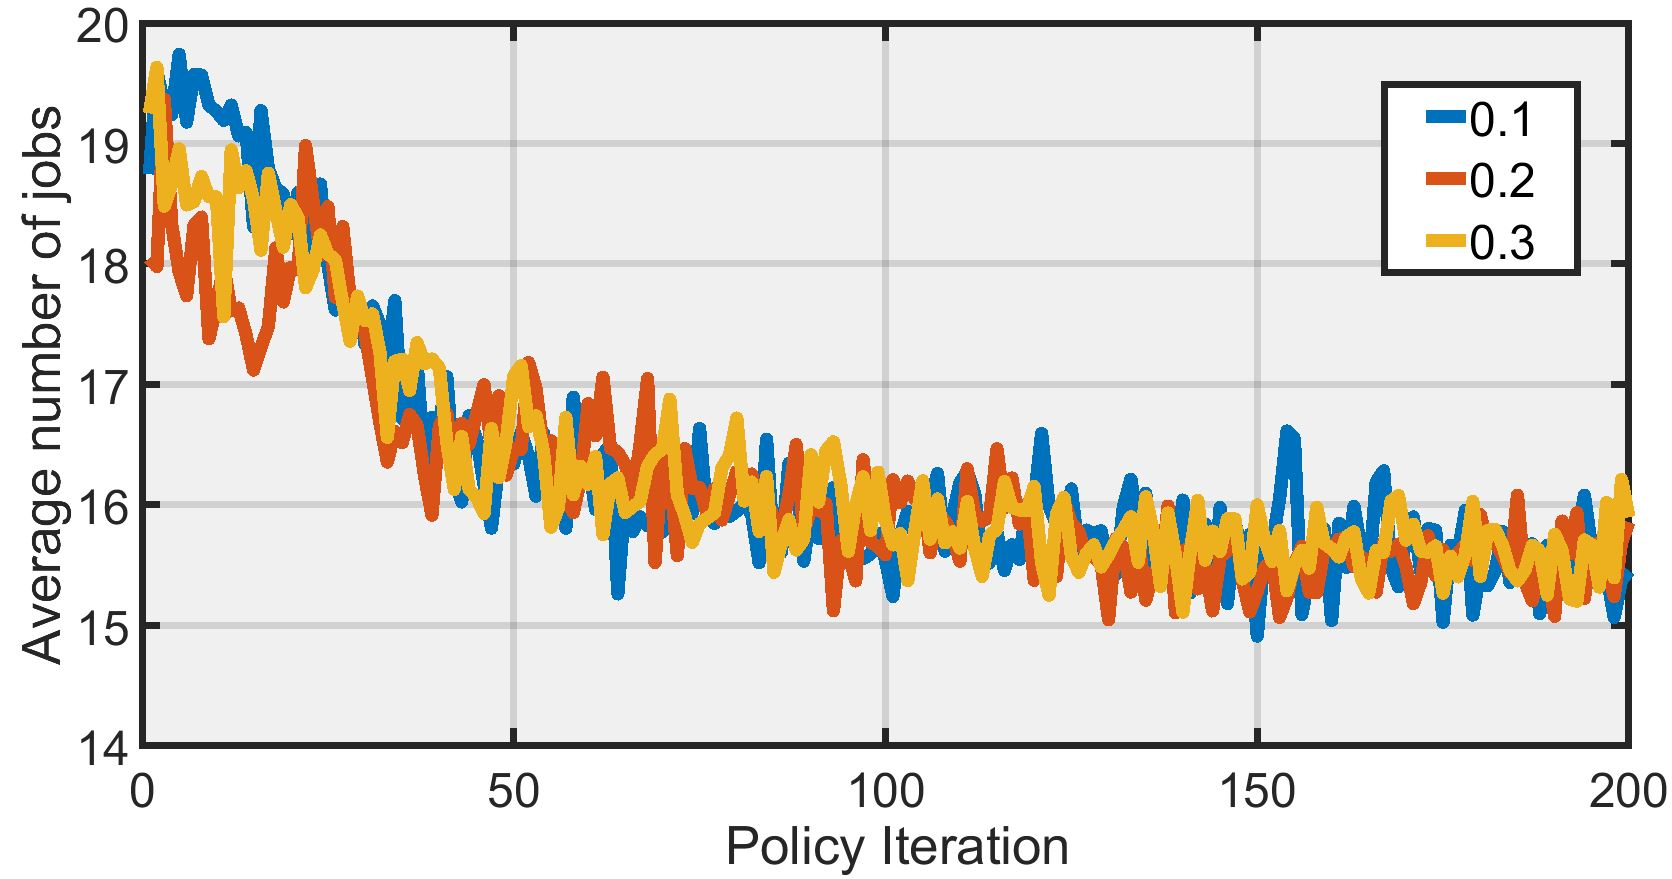
\includegraphics[width=0.45\textwidth, height=0.25\textwidth ]{Paper_clip}
     }
     \hfill
     \subfloat[Percentage of optimal actions \label{subfig-2:clip2}]{%
       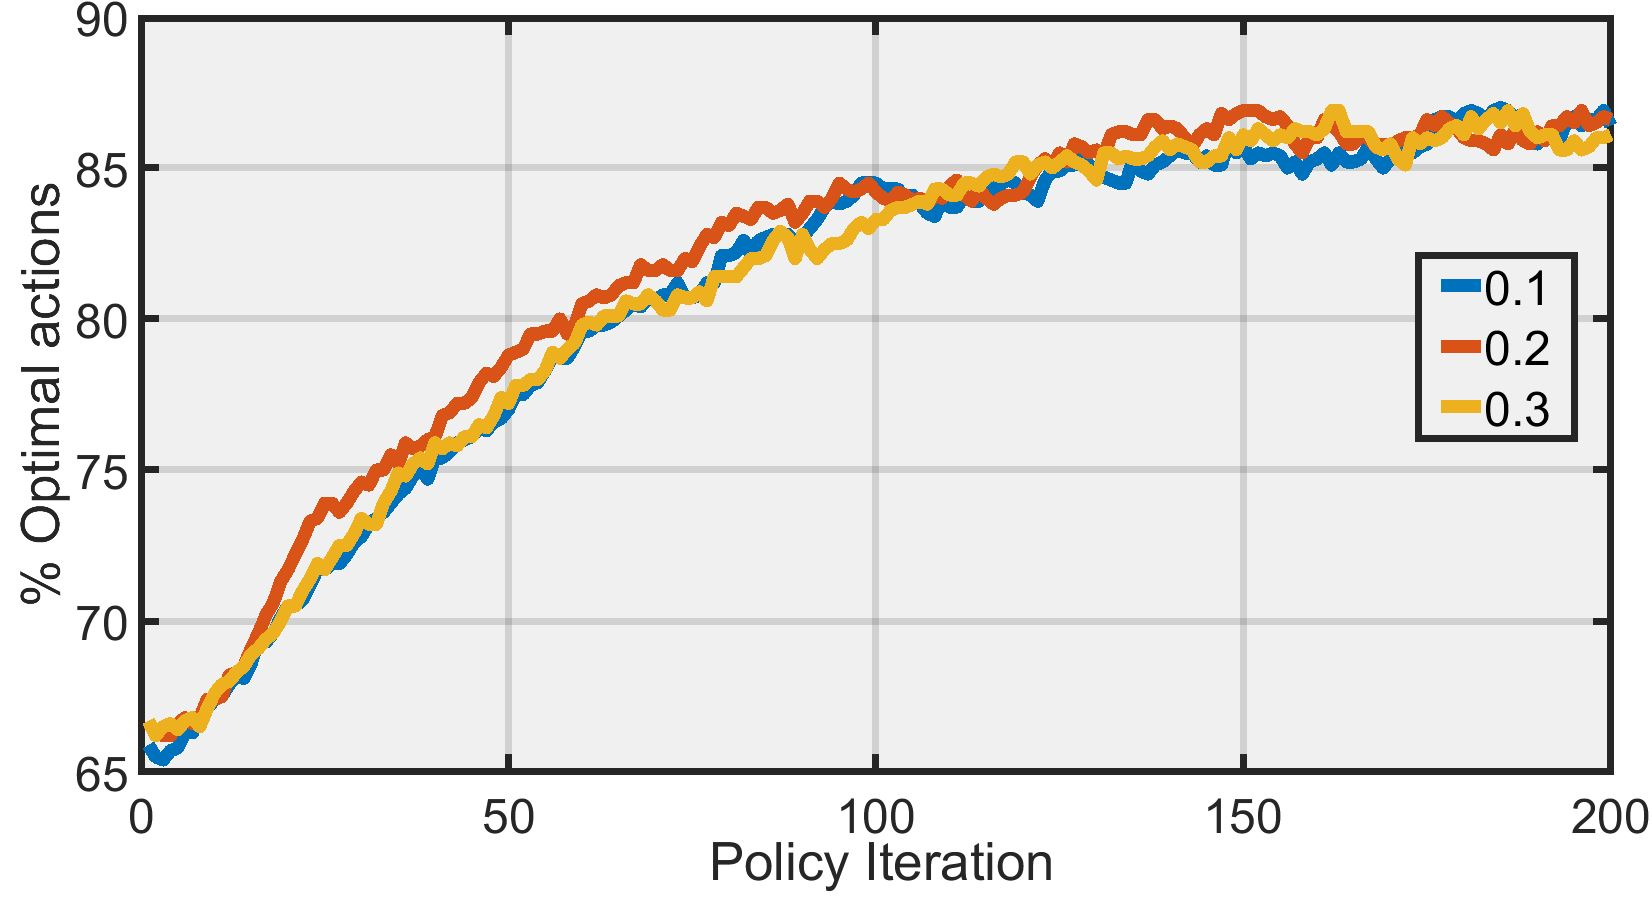
\includegraphics[width=0.45\textwidth, height=0.25\textwidth ]{Paper_clip_opt}
     }
     \caption{ Varying the clipping parameter within $\epsilon = \{0.1, 0.2, 0.3\}$ does not have  significant effect on learning.}
     \label{fig:clip}
   \end{figure}




Now we test dependency on number of episodes $E$ and their duration $T$. In Figure \ref{subfig:TE1} we fix number of episodes/actors to $N=25$ and test how the learning process depends on an episode horizon $T$. We observe that increasing horizon more than $T=40000$ does not yield further improvement. Next we fix total sample size to $T\times N = 10^9$ and examine the trade-off between number of episodes $N$ and an episode duration $T$.    In Figure \ref{subfig:TE2} we show learning curves for three sets of parameters $\{(T=10000, N=100), (T=20000, N=50), (T=40000, N=25)\}$. We observe that $ T=20000$ and $N=50$ is the best combination.


   \begin{figure}[!ht]
     \subfloat[  Results for different values of $T$ if number of actors is fixed $N=25$. \label{subfig:TE1}]{%
       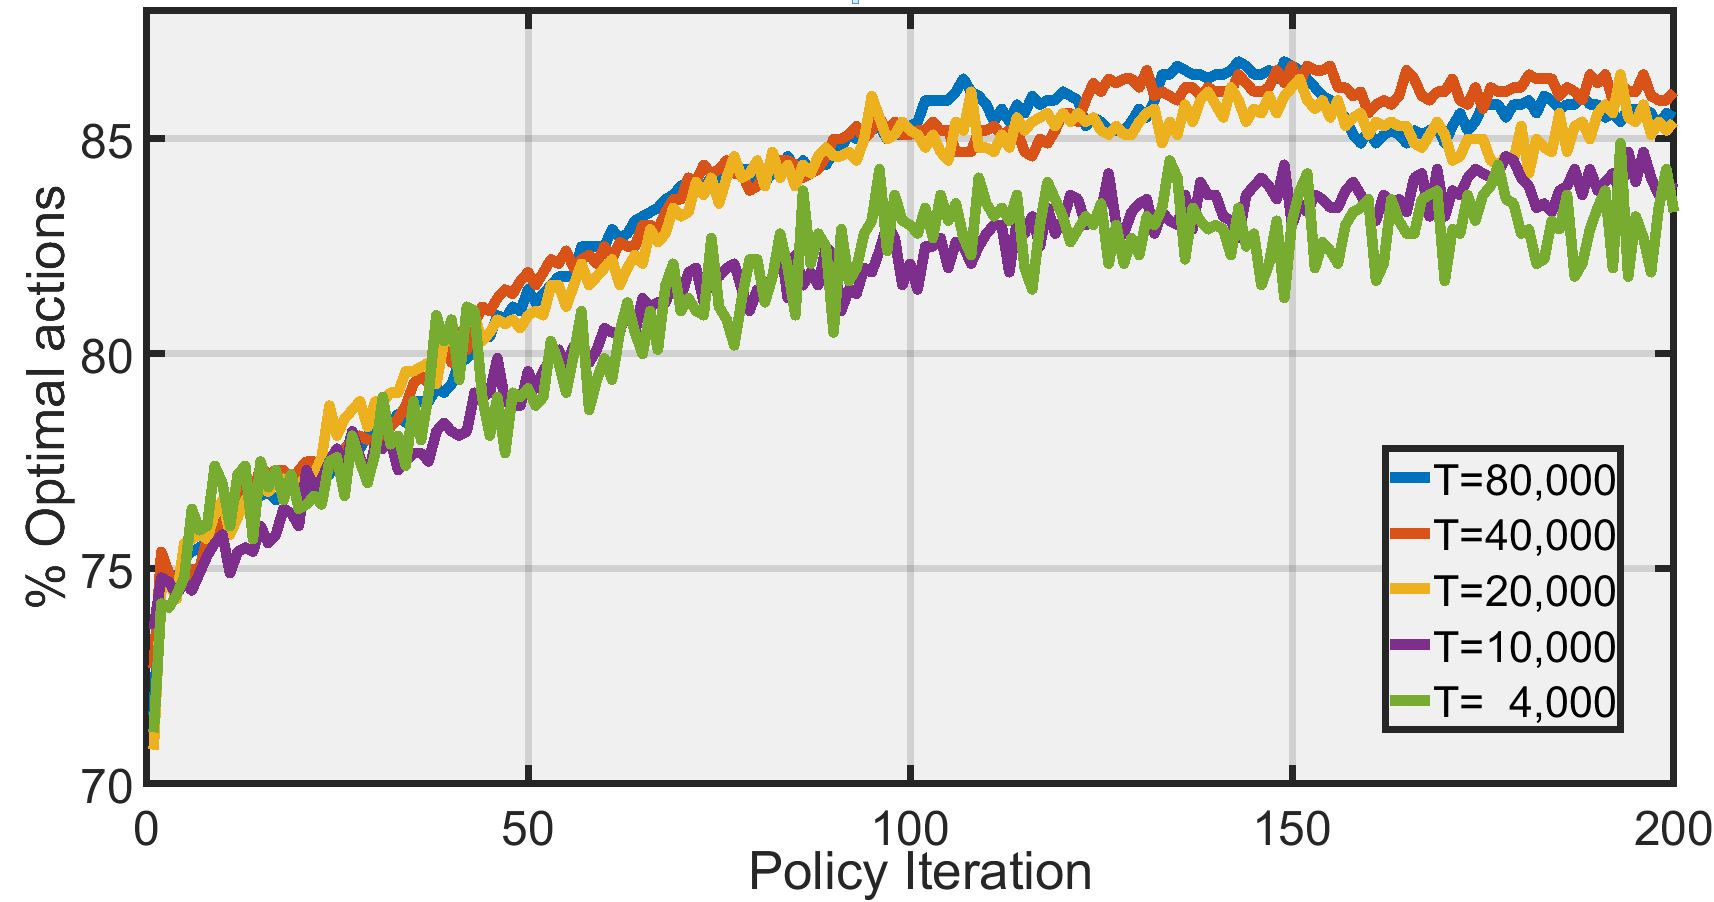
\includegraphics[width=0.45\textwidth, height=0.25\textwidth ]{Paper_SC_opt}
     }
     \hfill
     \subfloat[Trade-off between the number of actors $N$ and horizon length $T$.\label{subfig:TE2}]{%
       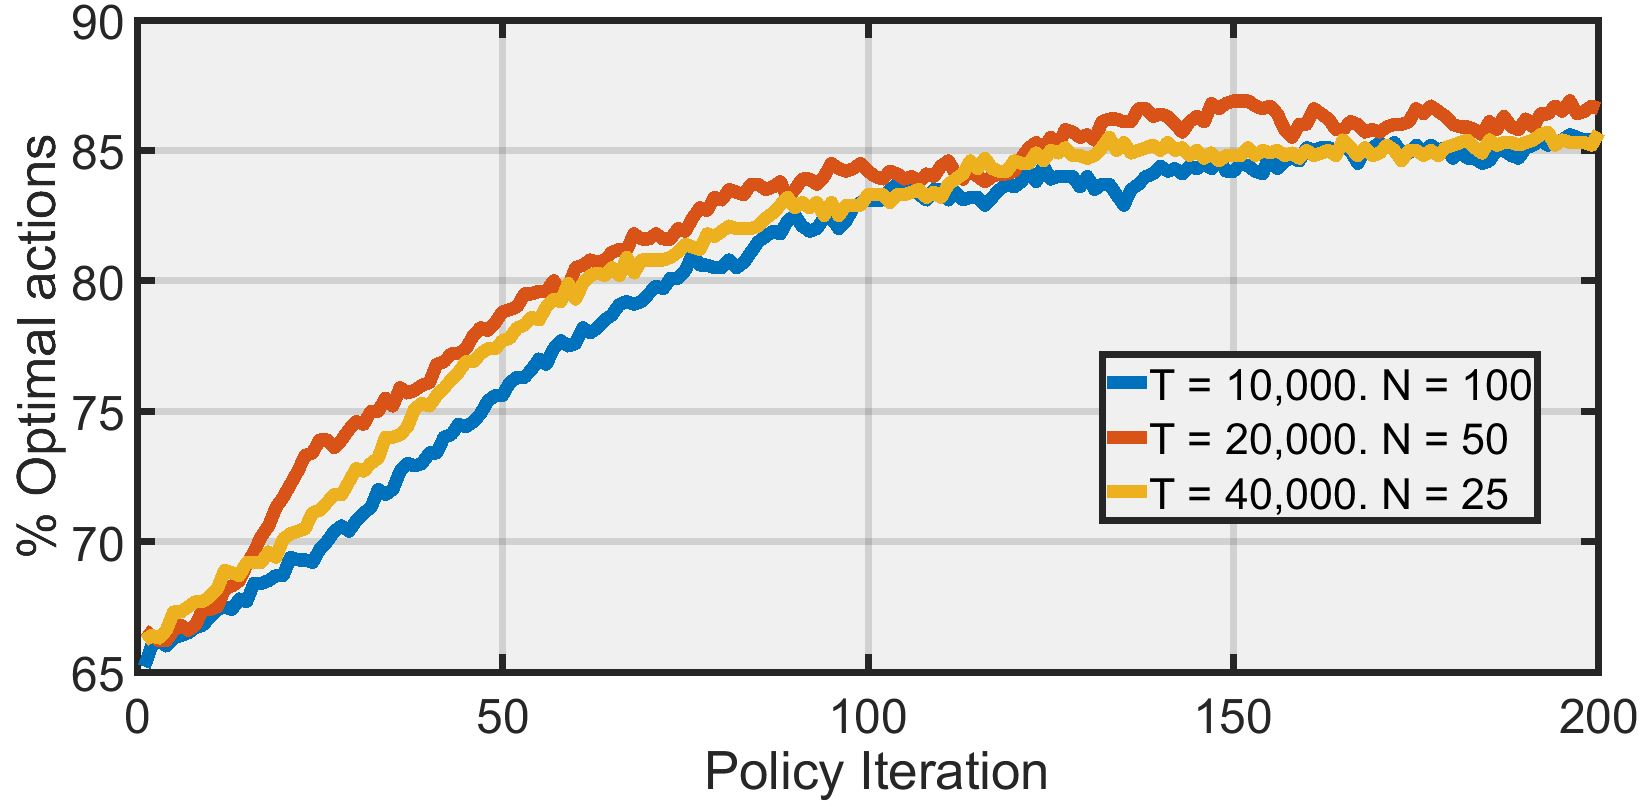
\includegraphics[width=0.45\textwidth, height=0.25\textwidth ]{PaperTE}
     }
     \caption{Effect of episode duration $T$ and number of actors $N$ on the learning process. }
     \label{fig:TE}
   \end{figure}



Another important parameter is discount factor $\beta$. We examine a discount factor jointly with GAE parameter $\lambda.$ In our tests parameters $\beta = 0.995$ and $\lambda = 0.97$ yield the best result.


\begin{figure}[H]
\centering%
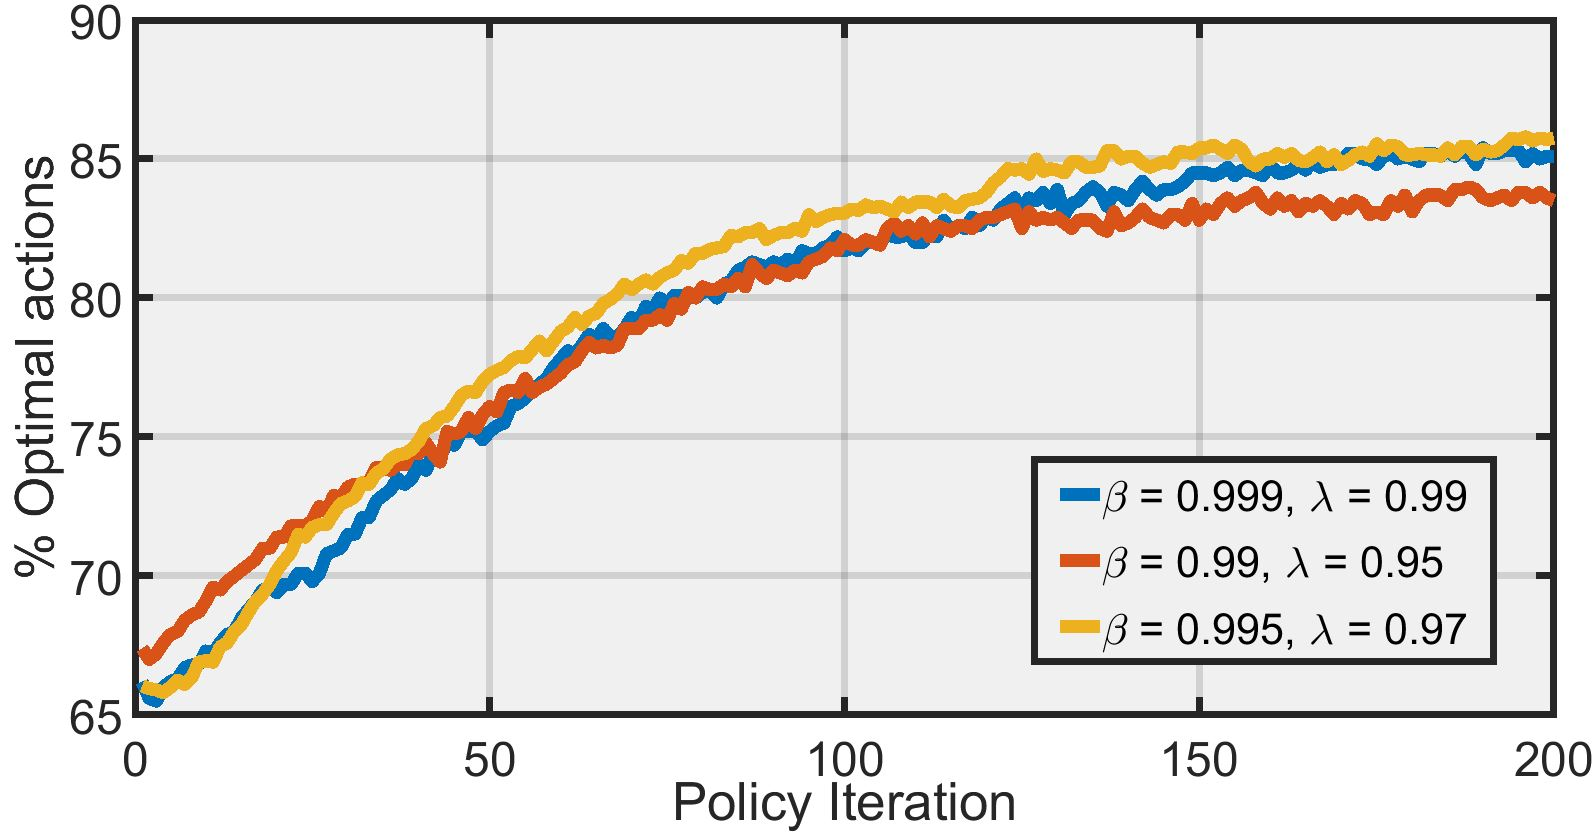
\includegraphics[width=0.55\textwidth, height=0.30\textwidth]{Paper_beta.JPG}
\caption[]{Effect of discount factor and GAE parameter.  }
\label{fig:beta}%
\end{figure}


\subsection{Learning Curves}








  \begin{figure}[H]
     \subfloat[Balanced heavy (BH) traffic\label{subfig-1:BH}]{%
       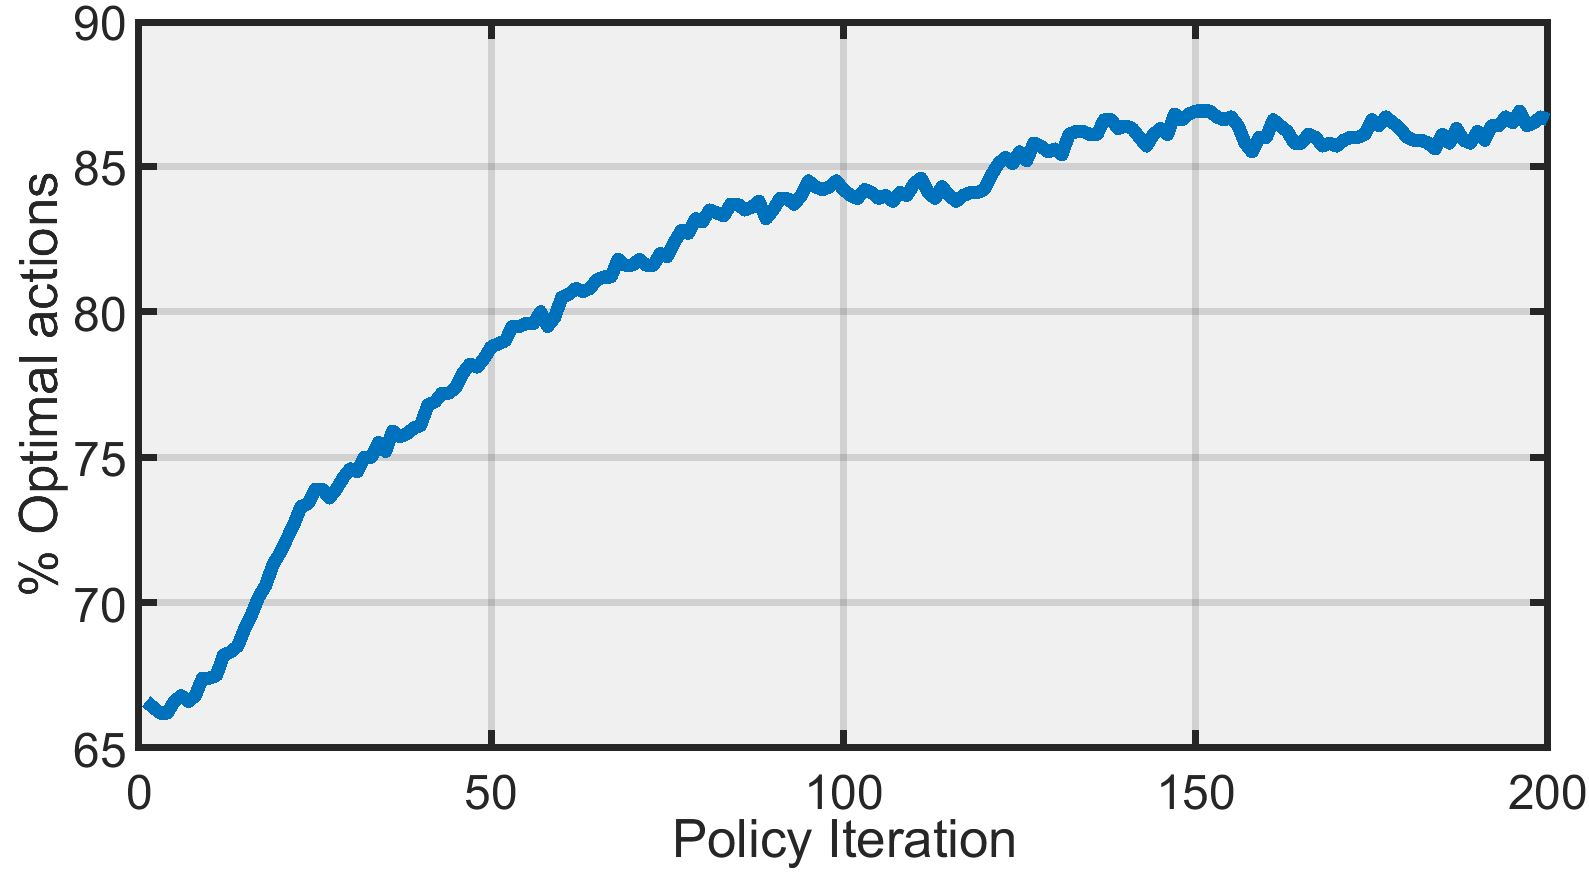
\includegraphics[ height=0.2\textwidth, width=0.35\textwidth]{Paper_BH_opt}
     }
     \subfloat[Balanced medium (BM) traffic\label{subfig-3:BM}]{%
       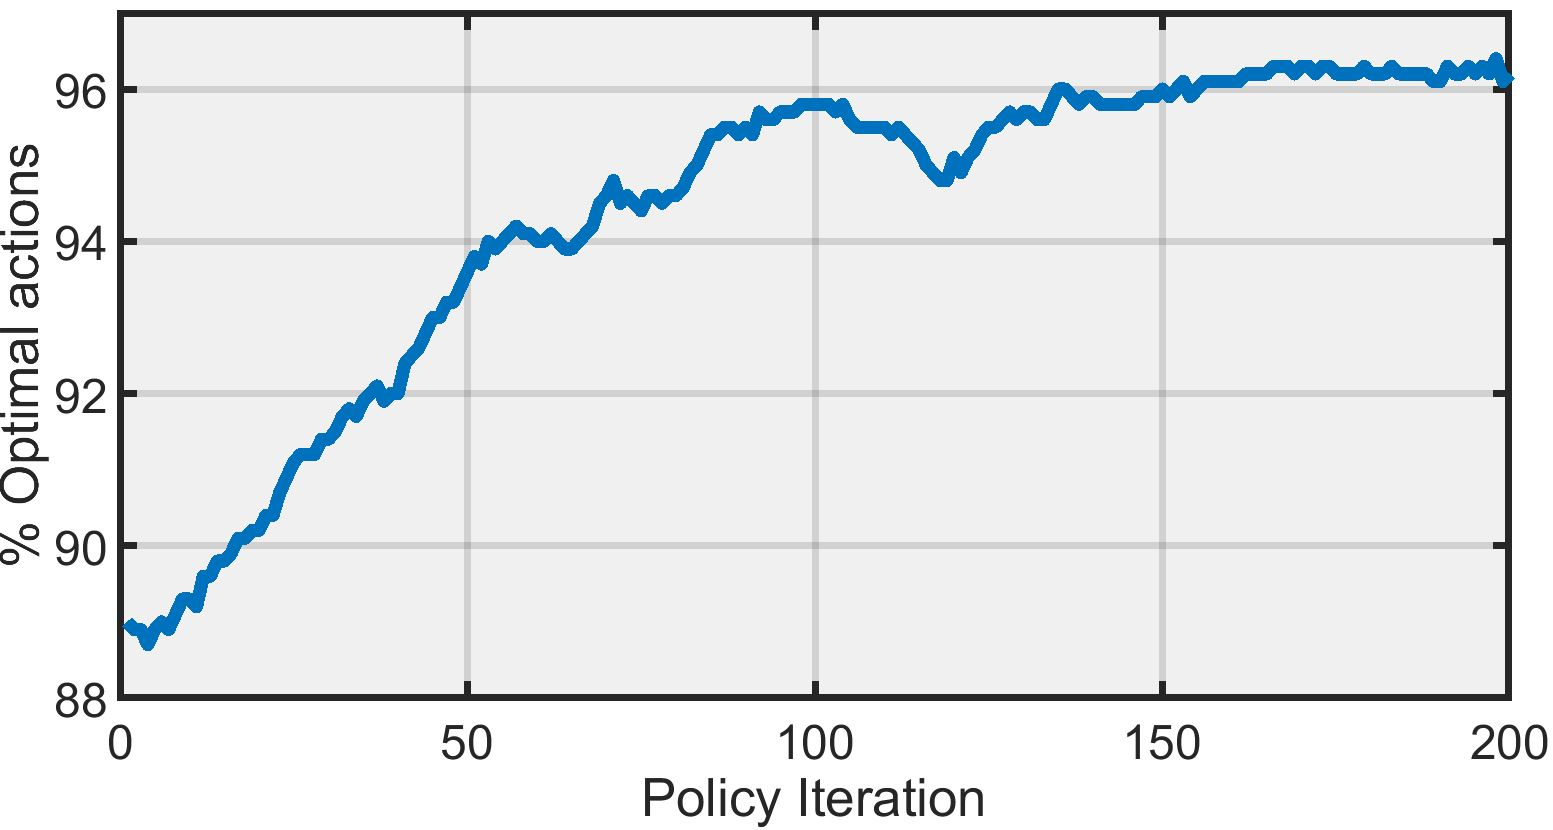
\includegraphics[  height=0.2\textwidth, width=0.35\textwidth]{Paper_BM_opt}
     } 
     \subfloat[Balanced low (BL) traffic\label{subfig-5:BL}]{%
       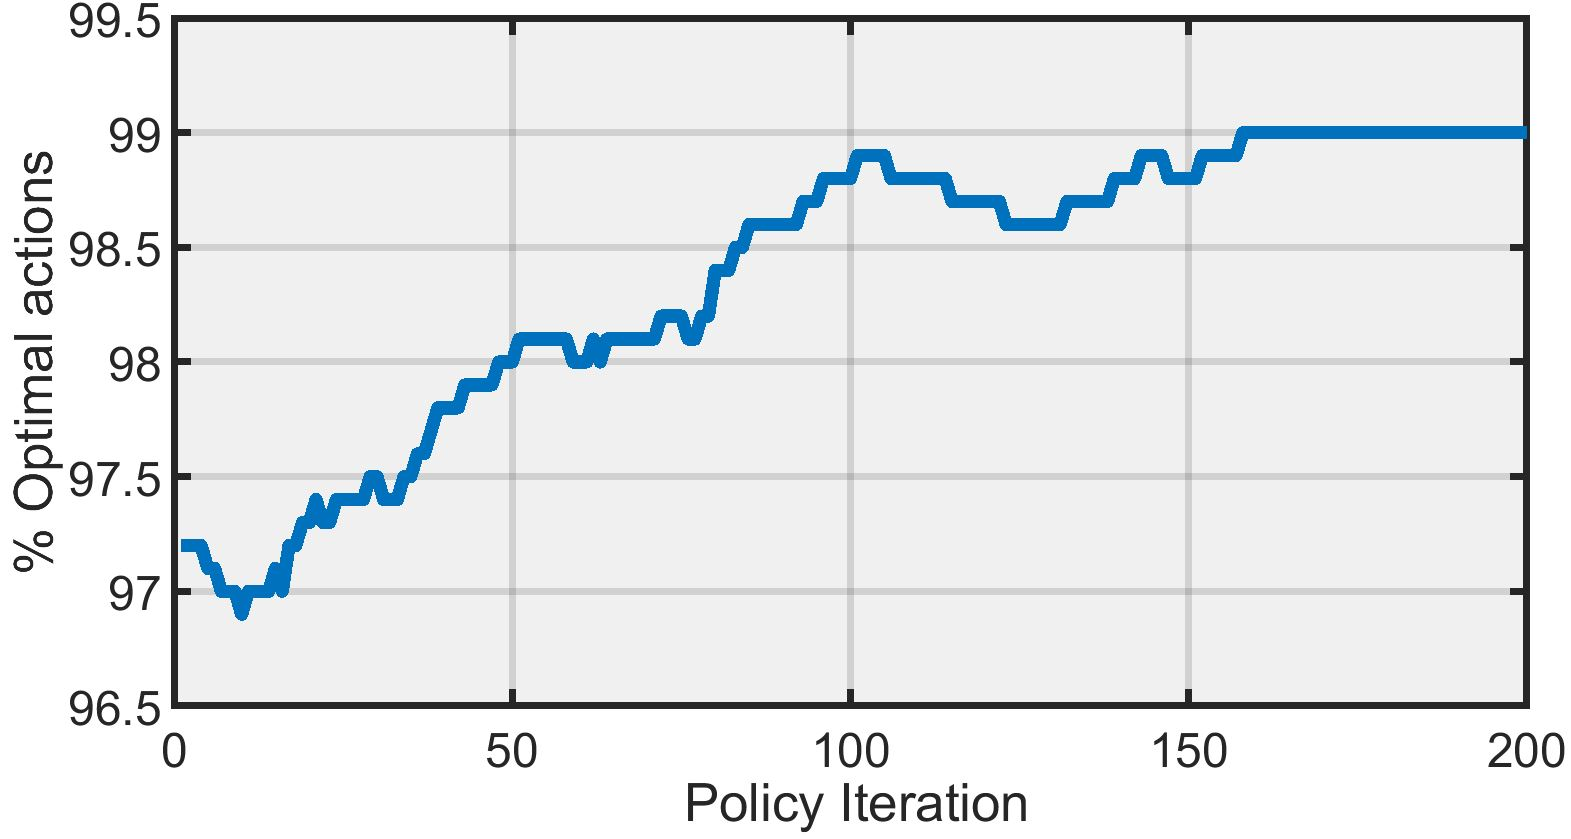
\includegraphics[  height=0.2\textwidth, width=0.35\textwidth]{Paper_BL_opt}
     }\\
     \subfloat[Imbalanced heavy (IH) traffic \label{subfig-2:IH}]{%
       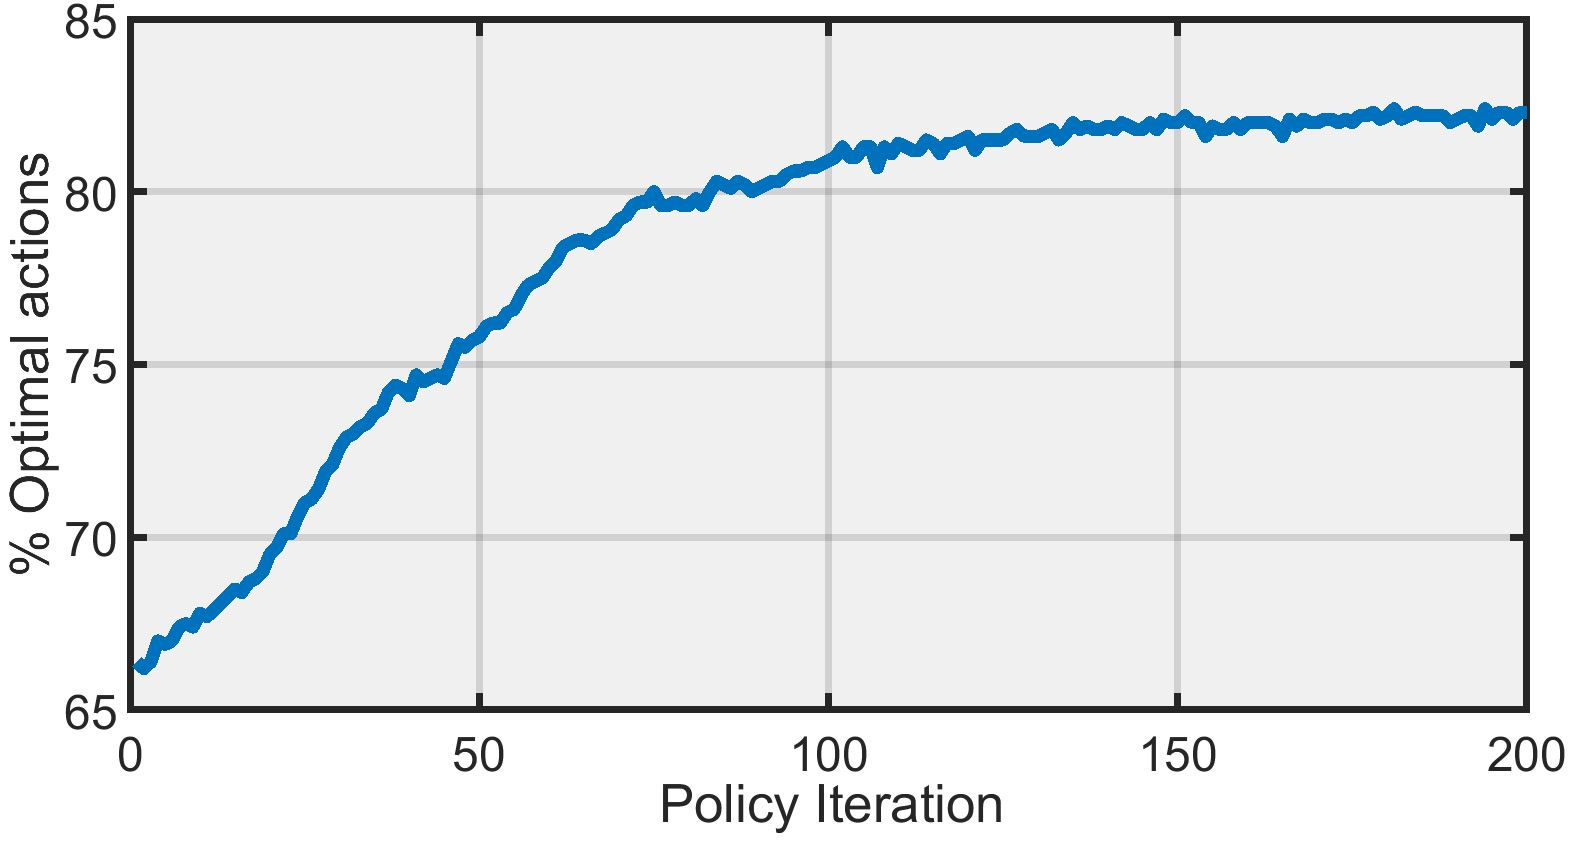
\includegraphics[ height=0.2\textwidth, width=0.35\textwidth]{Paper_IH_opt}
     }
     \subfloat[Imbalanced medium (IM) traffic \label{subfig-4:IM}]{%
       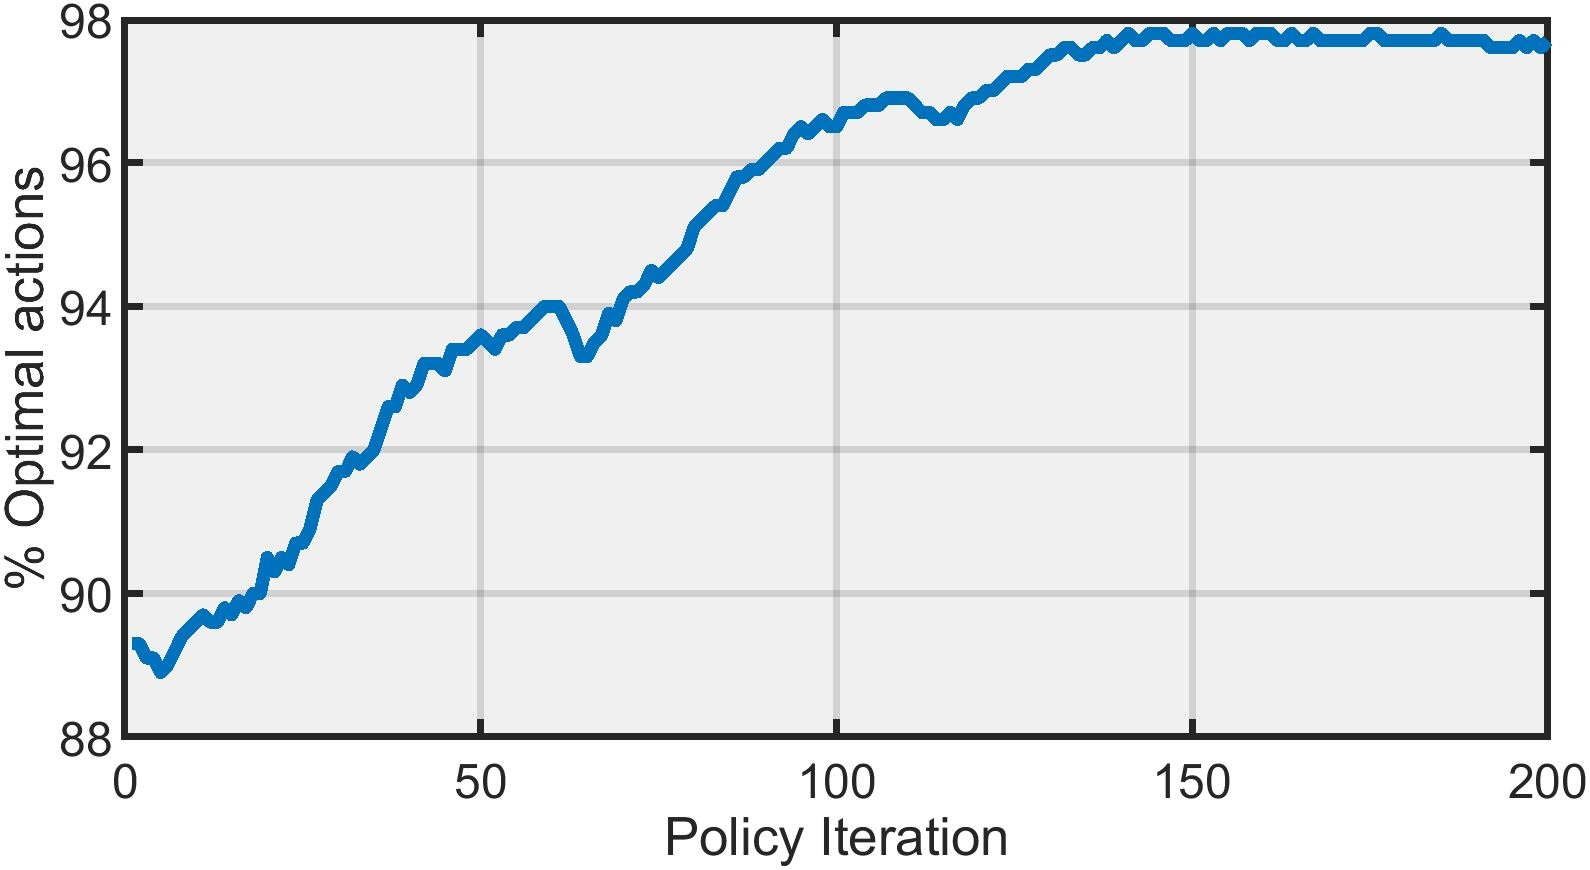
\includegraphics[ height=0.2\textwidth, width=0.35\textwidth]{Paper_IM_opt}
     }
     \subfloat[Imbalanced low (IL) traffic \label{subfig-6:IL}]{%
       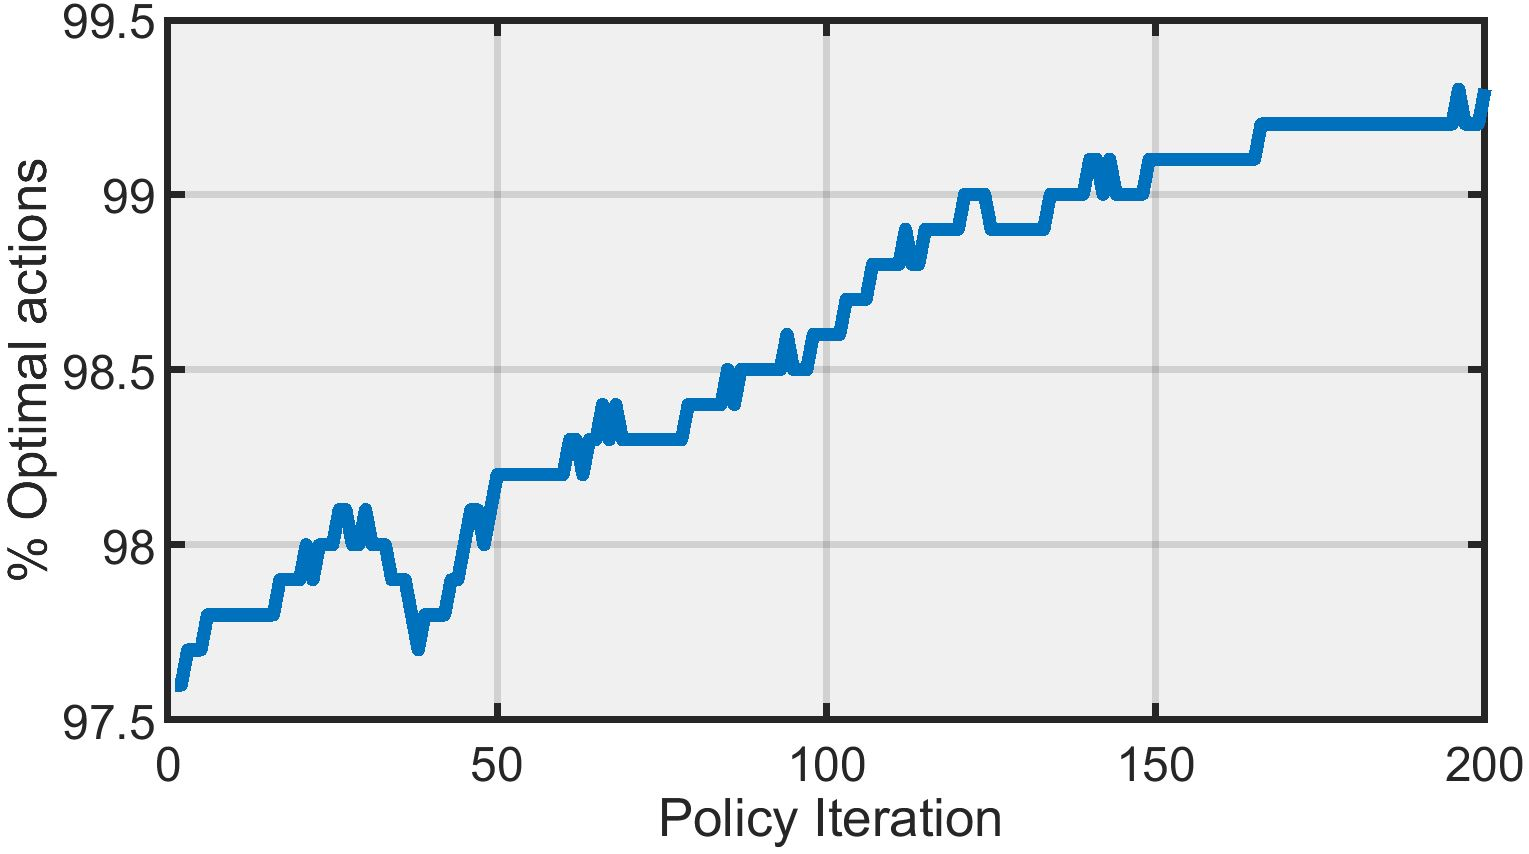
\includegraphics[ height=0.2\textwidth, width=0.35\textwidth]{Paper_IL_opt}
     }
     \caption{Learning of optimal actions. Results for the criss-cross network of Figure \ref{fig:cc} under different
traffic regimes.}
     \label{fig:cc_opt}
   \end{figure}


\begin{figure}[H]
    \subfloat[6-classes network \label{subfig-6:IL}]{%
       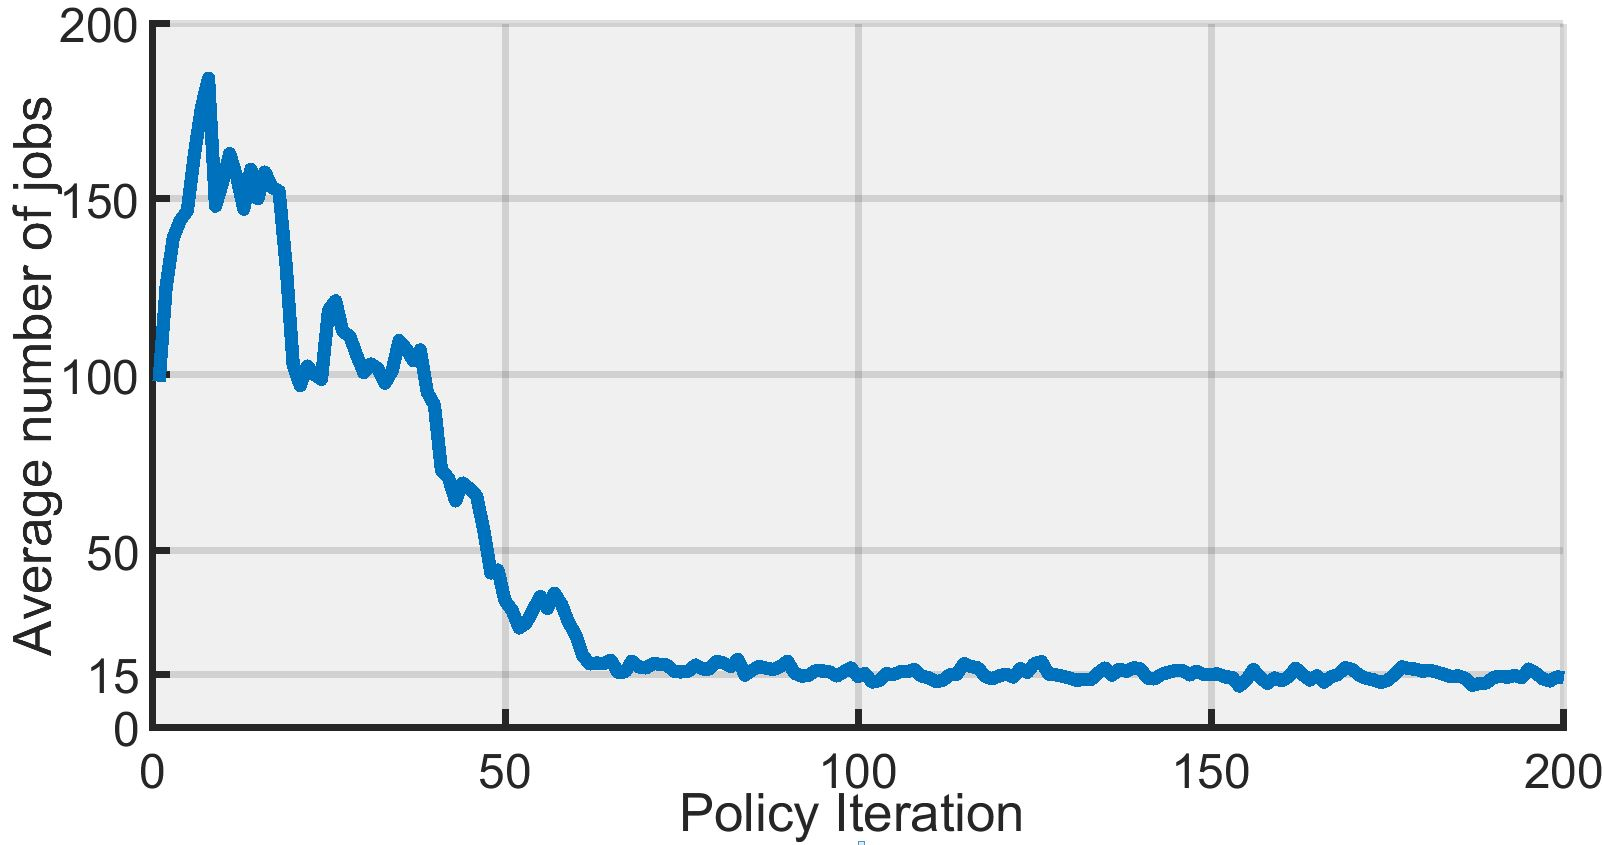
\includegraphics[height=0.2\textwidth, width=0.35\textwidth]{Paper6classes}
     }
     \subfloat[9-classes network \label{subfig-4:IM}]{%
       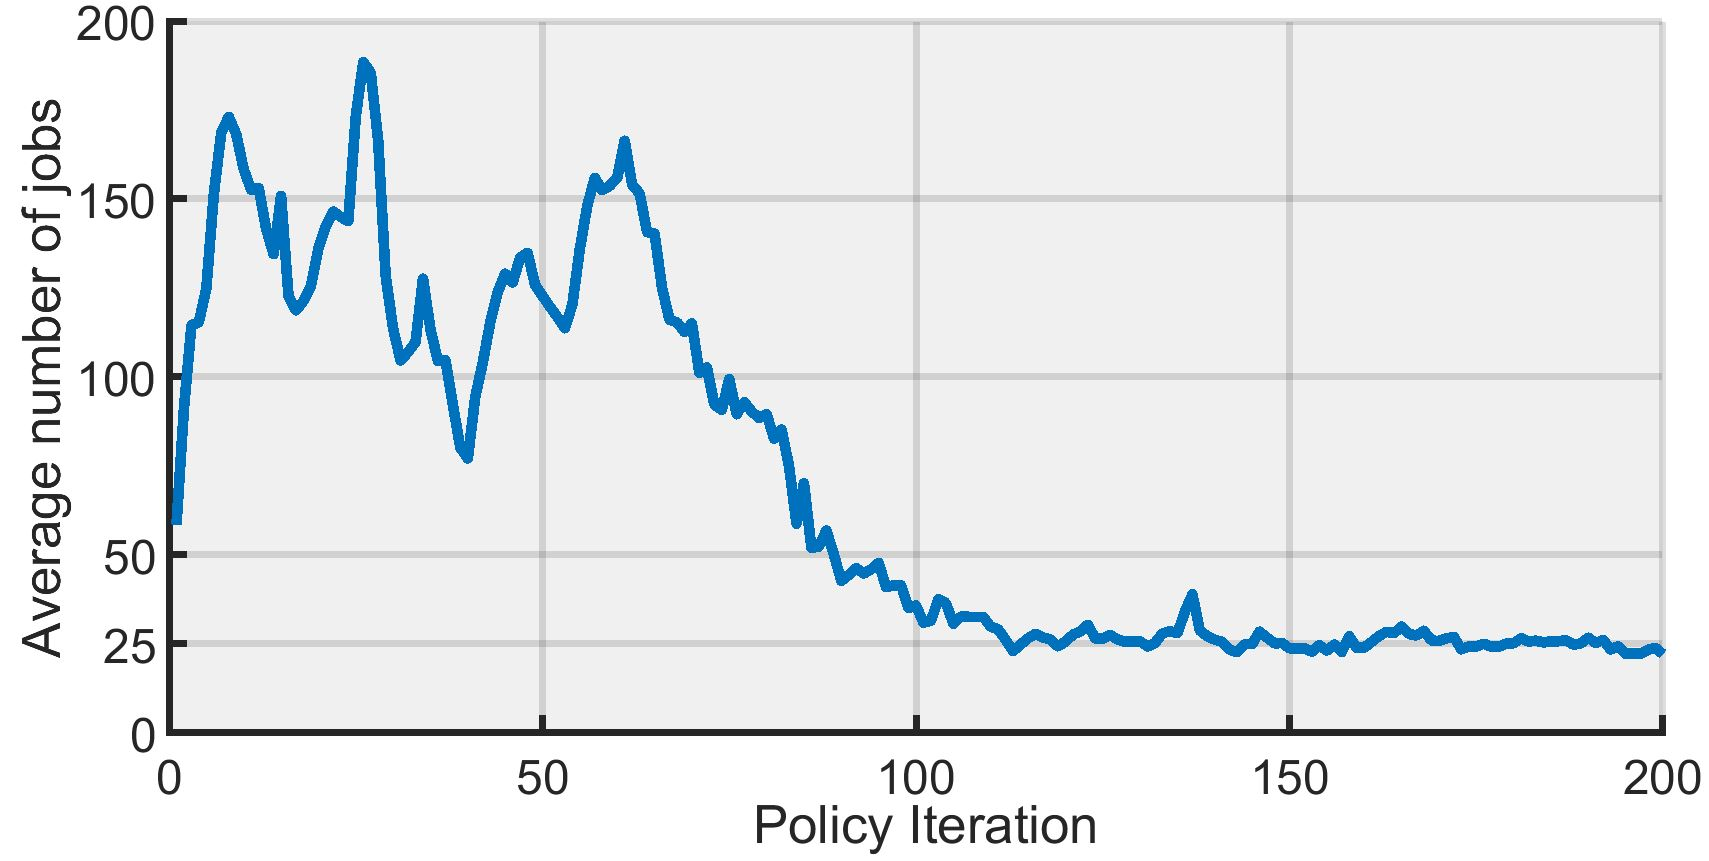
\includegraphics[height=0.2\textwidth, width=0.35\textwidth]{Paper9classes}
     }
     \subfloat[12-classes network \label{subfig-2:IH}]{%
       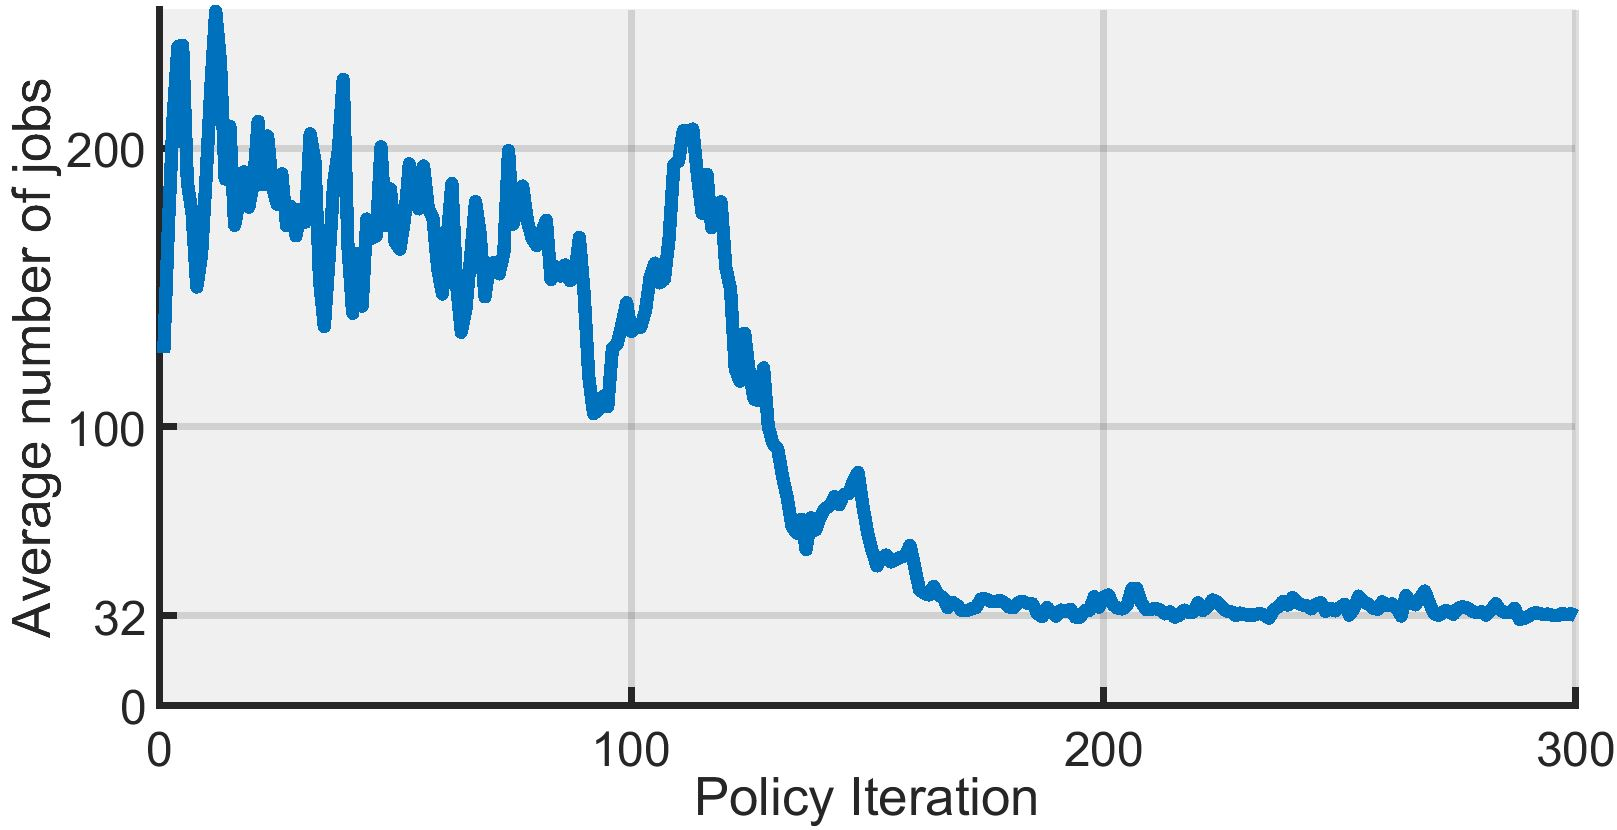
\includegraphics[height=0.2\textwidth, width=0.35\textwidth]{Paper12classes}
     }\\
 \subfloat[15-classes network\label{subfig-5:BL}]{%
       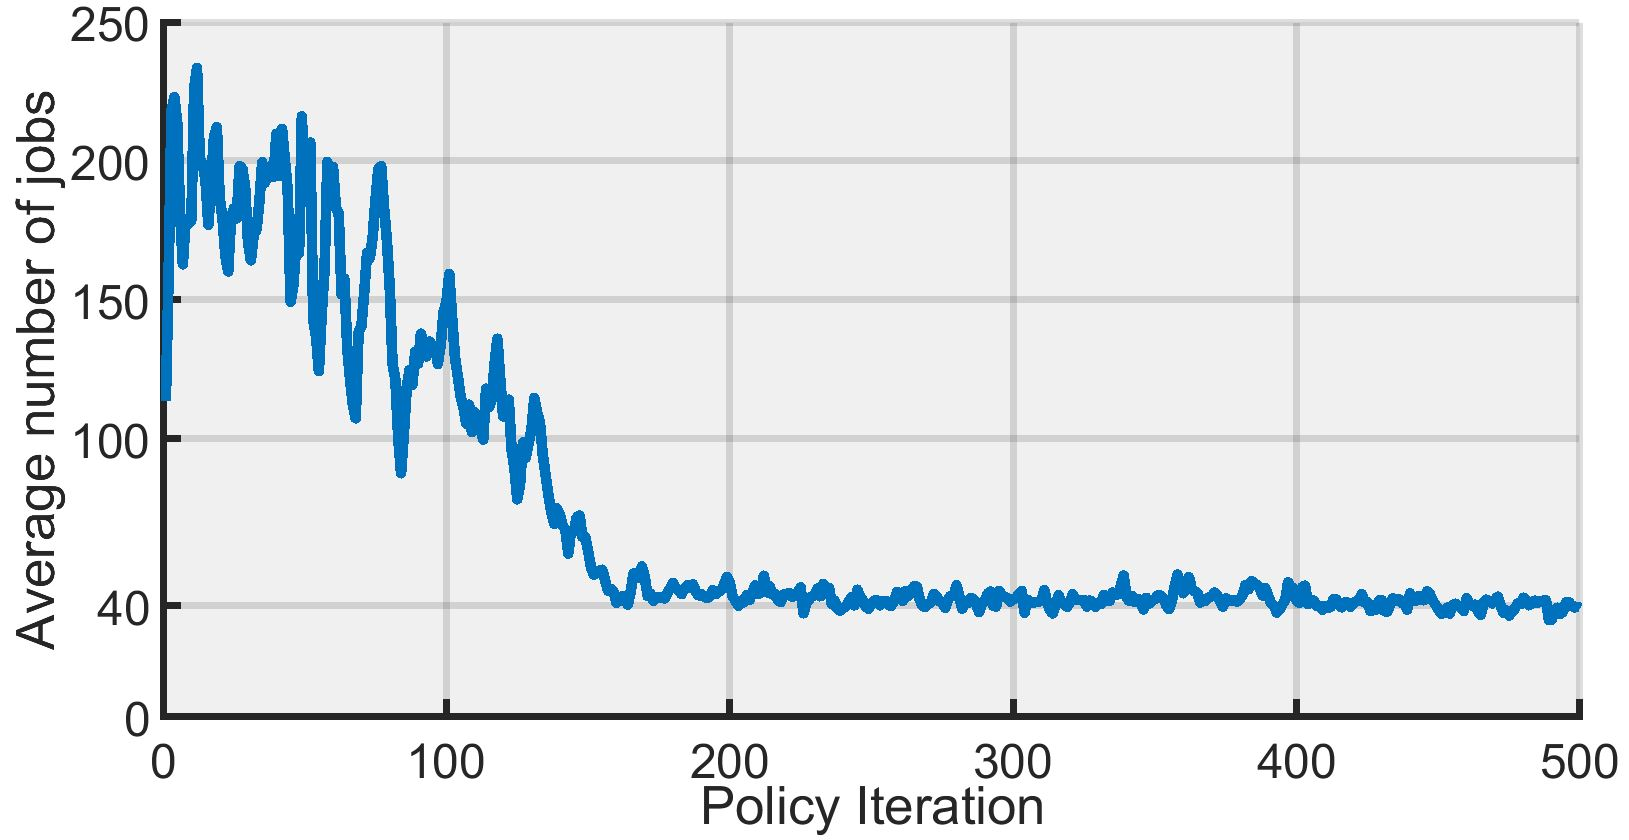
\includegraphics[ height=0.2\textwidth, width=0.35\textwidth]{Paper15classes}
     }
  \subfloat[18-classes network\label{subfig-3:BM}]{%
       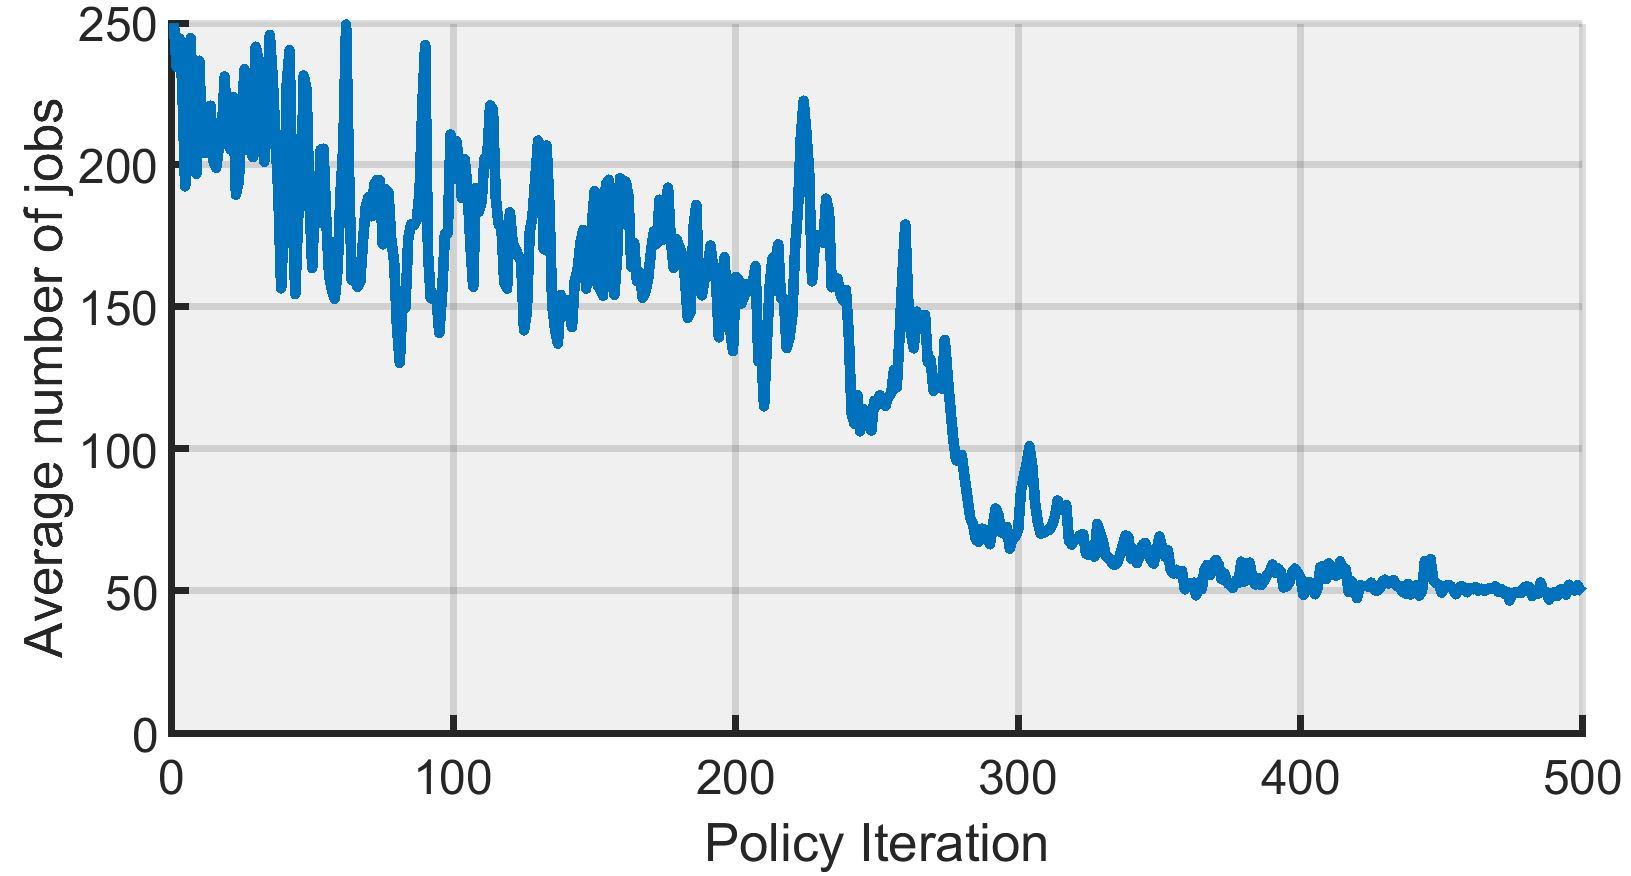
\includegraphics[ height=0.2\textwidth, width=0.35\textwidth]{Paper18classes}
     }
     \subfloat[21-classes network\label{subfig-1:BH}]{%
       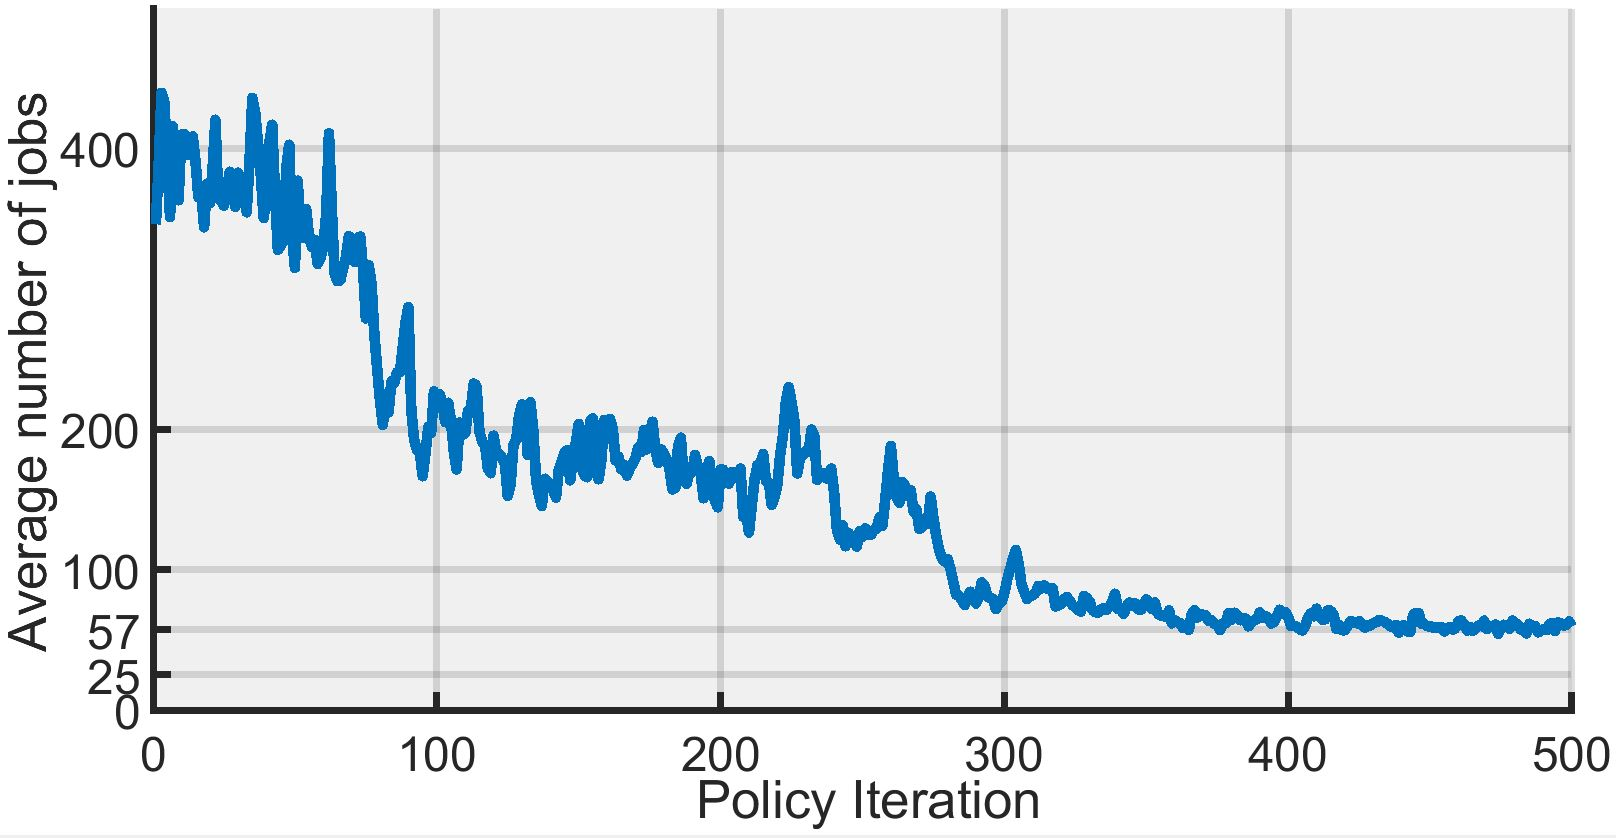
\includegraphics[ height=0.2\textwidth, width=0.35\textwidth]{Paper21classes}
     }


\caption{Learning curves for the 6-class extended network of Figure \ref{fig1}}
     \label{fig:ext_ac}
   \end{figure}


\begin{figure}[H]
    \subfloat[6-classes network \label{subfig-6:IL}]{%
       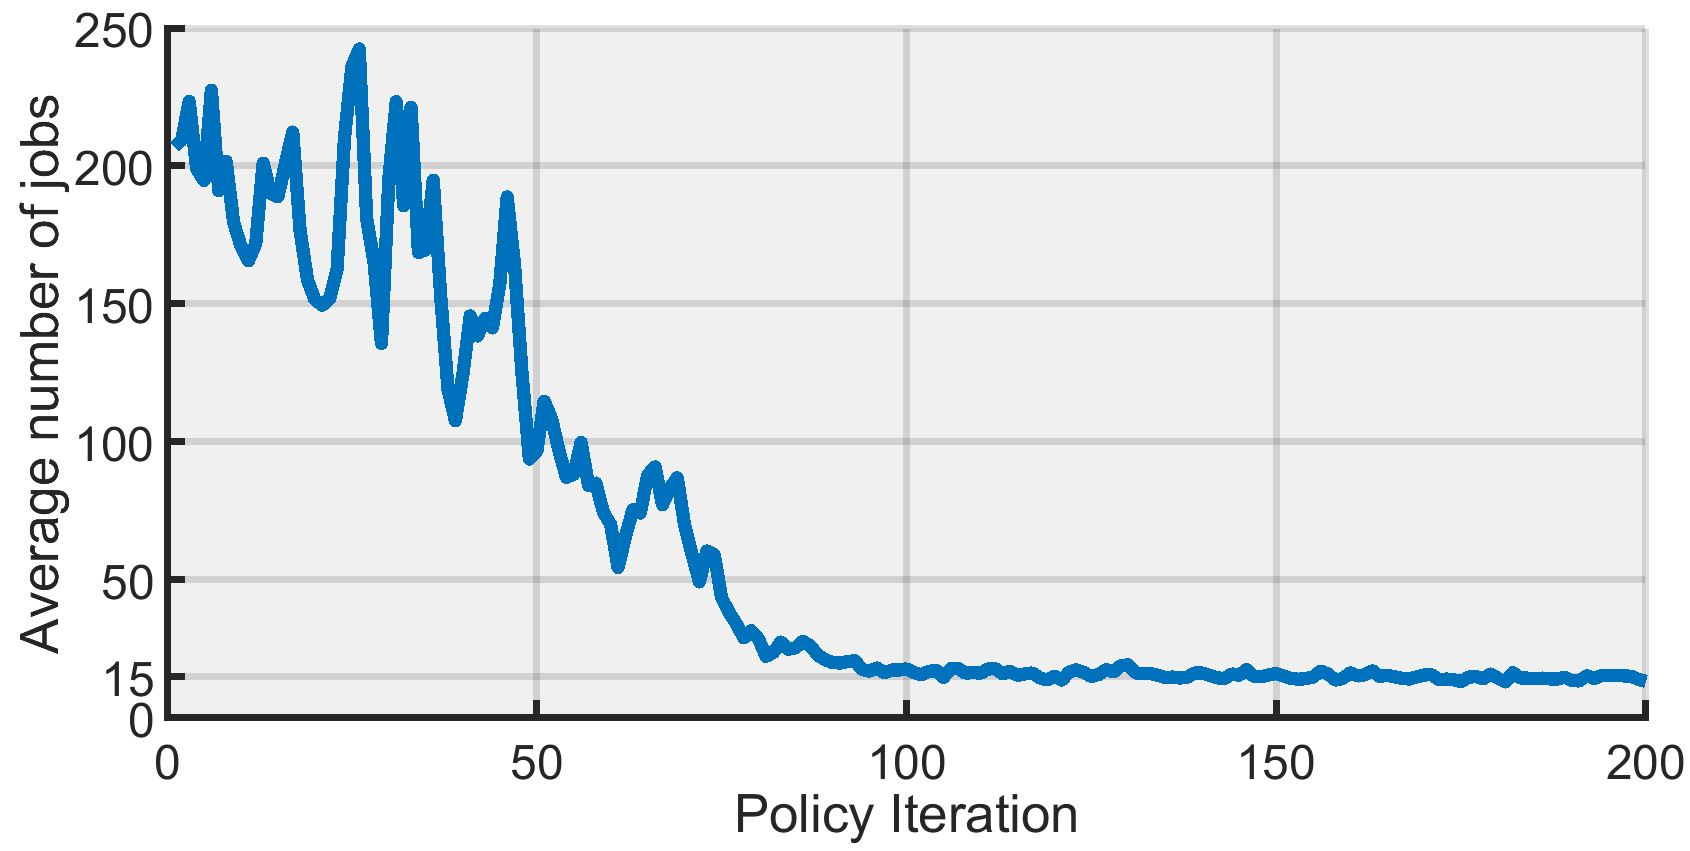
\includegraphics[height=0.2\textwidth, width=0.35\textwidth]{Paper6classes_re}
     }
     \subfloat[9-classes network \label{subfig-4:IM}]{%
       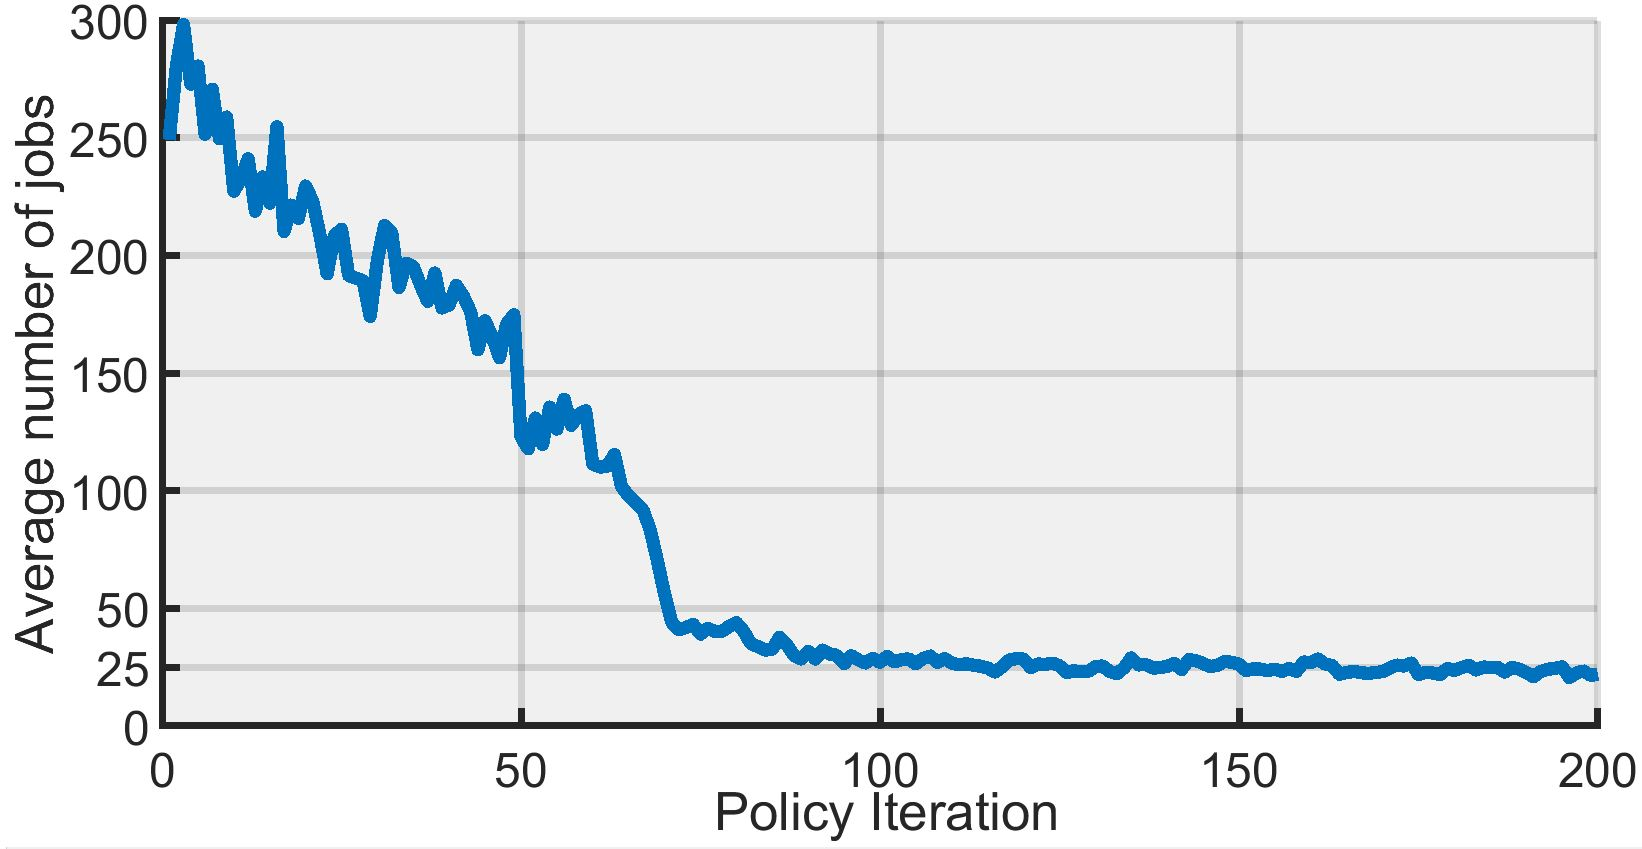
\includegraphics[height=0.2\textwidth, width=0.35\textwidth]{Paper9classes_re}
     }
     \subfloat[12-classes network \label{subfig-2:IH}]{%
       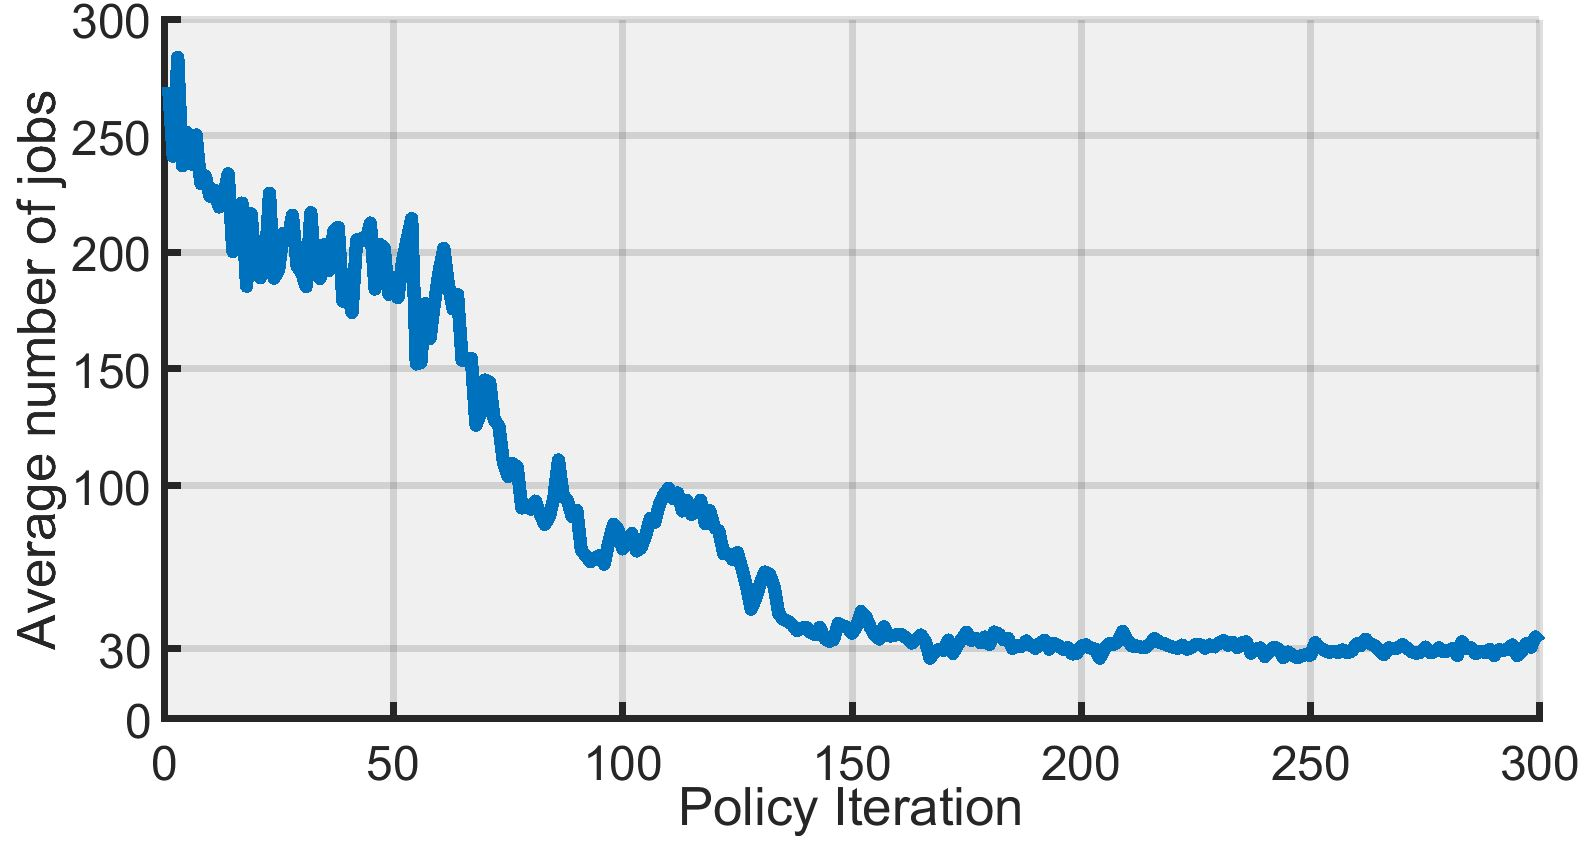
\includegraphics[height=0.2\textwidth, width=0.35\textwidth]{Paper12classes_re}
     }\\
 \subfloat[15-classes network\label{subfig-5:BL}]{%
       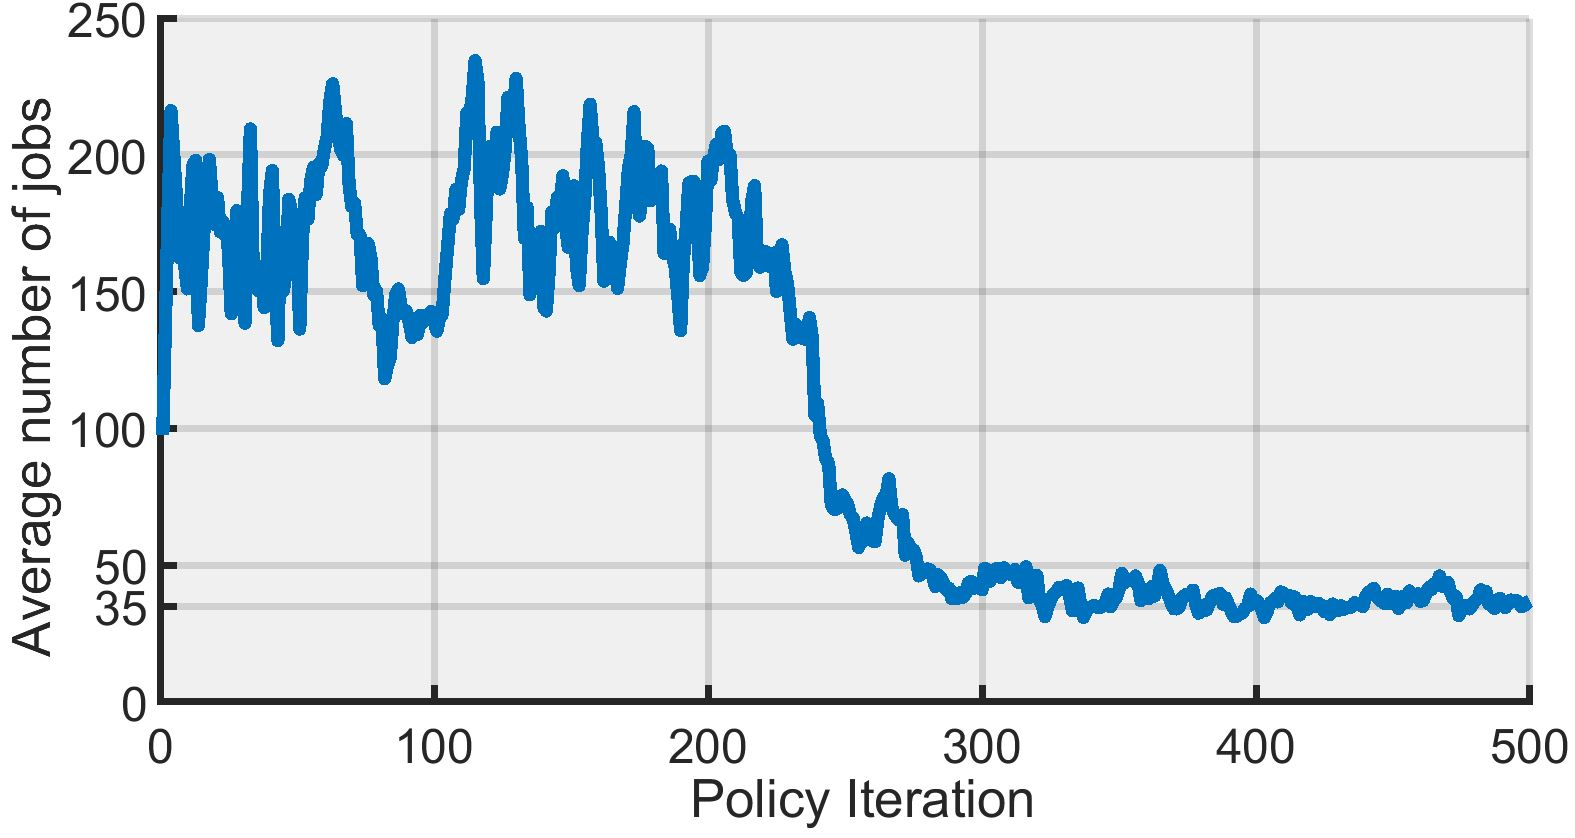
\includegraphics[ height=0.2\textwidth, width=0.35\textwidth]{Paper15classes_re}
     }
  \subfloat[18-classes network\label{subfig-3:BM}]{%
       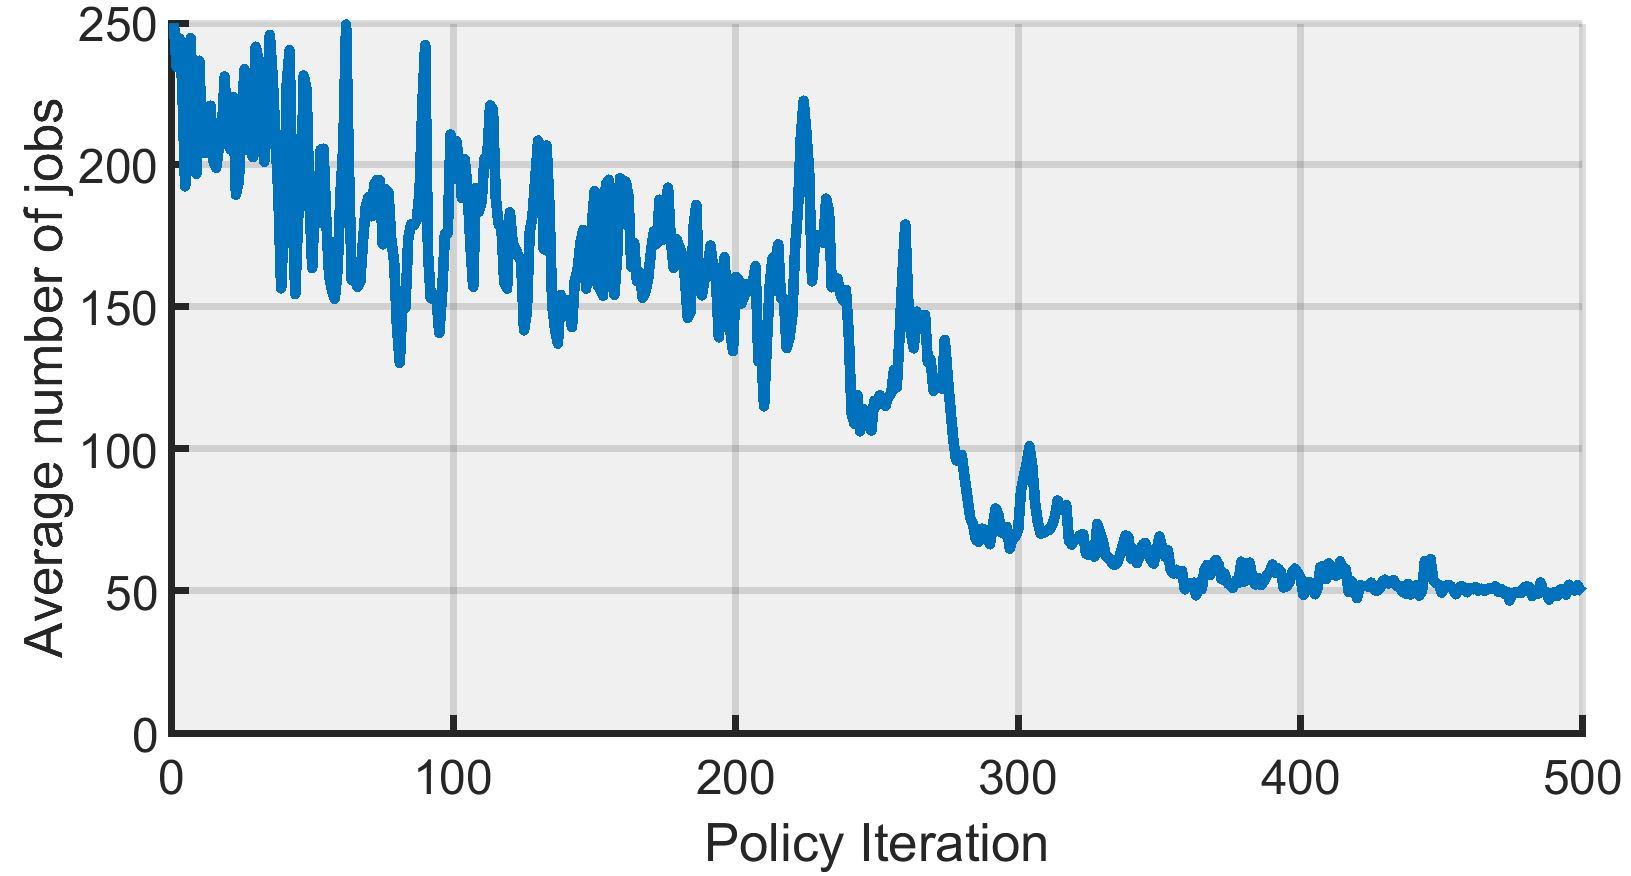
\includegraphics[ height=0.2\textwidth, width=0.35\textwidth]{Paper18classes}
     }
     \subfloat[21-classes network\label{subfig-1:BH}]{%
       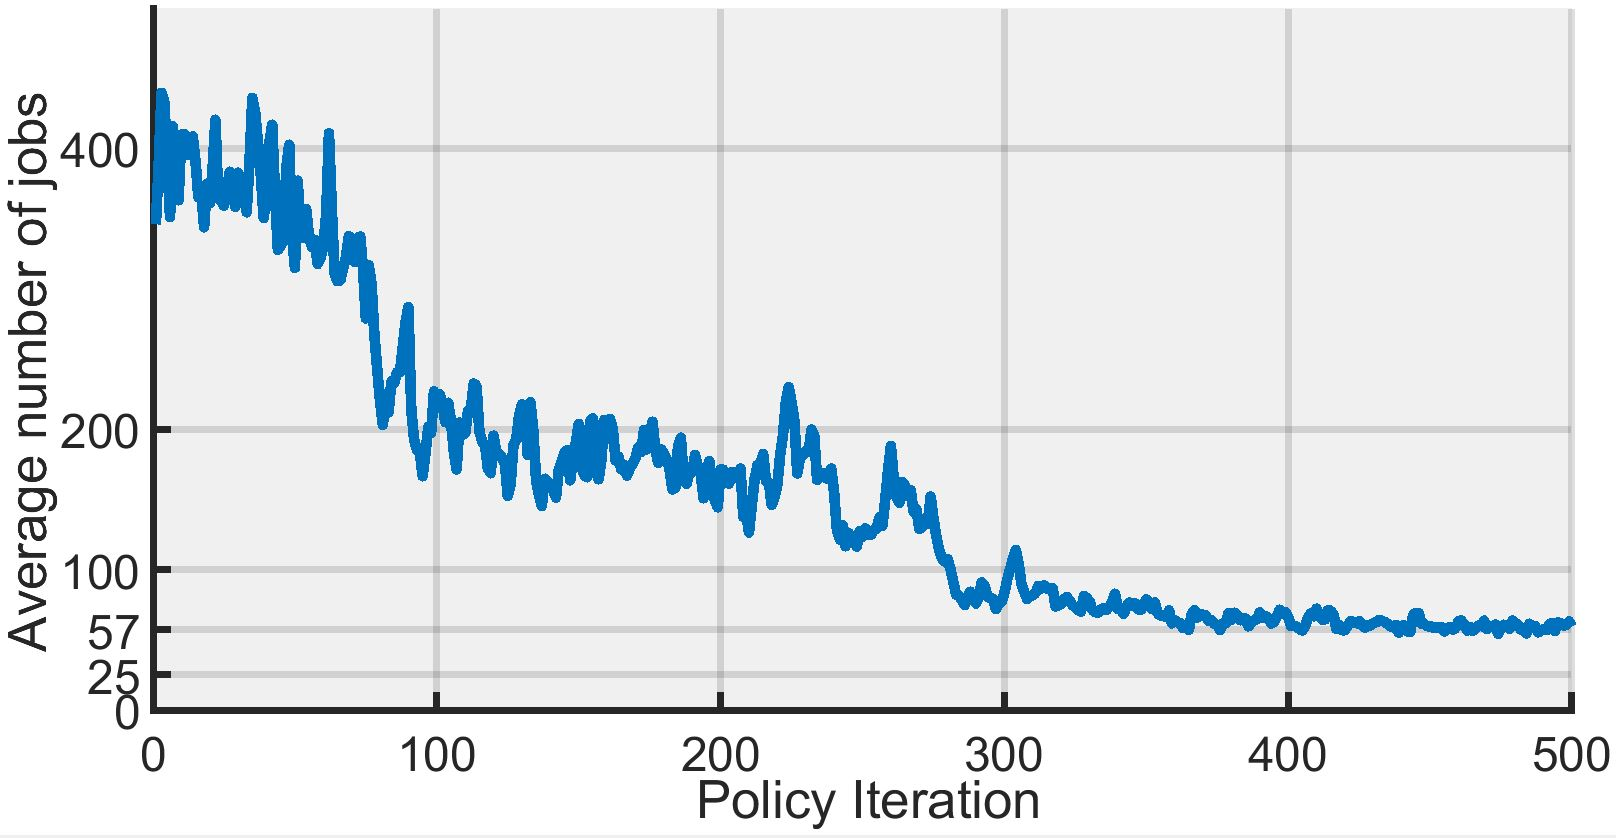
\includegraphics[ height=0.2\textwidth, width=0.35\textwidth]{Paper21classes}
     }


\caption{Learning curves for the reentrant extended network of Figure \ref{fig2}}
     \label{fig:reent_ac}
   \end{figure}
   
   \subsection{Choosing initial states for simulation}

In the Algorithm \ref{alg2} we use finite episodes to estimate the expectation of the advantage function over the stationary distribution of the current policy. To run the simulations one needs to specify how to choose initial states for the episodes.

\begin{algorithm}[h]
\SetAlgoLined
\KwResult{policy $\pi_{I}$ }
 Initialization: policy $\pi_{0}$,  buffer $\mathbb{B}=\emptyset$\;
 Run policy $\pi_{0}$ for $T$ timesteps\;
 Sample uniformly at random $100\times N$ states from the simulation of policy $\pi_{0}$\;
 Add $100\times N$ states to $\mathbb{B}$\;

 \For{ policy iteration $= 1, 2, ..., I$}{

  Sample uniformly at random $N$ states $\{x^1, x^2, ..., x^N\}$ from $\mathbb{B}$;

  \For{ $s = 1, 2, ..., N$}{
  \If{ $\sum\limits_{j=1}^J x^s_j >\Lambda$ }
  { $x^s = (0,...,0)$;
  }
  }


  \For{ actor  $ s= 1, 2, ..., N$}{
  Initialize episode at state $x^s$;
 }
  Sample uniformly at random $100\times N$ states from policy $\pi_{i}$ simulation\;
 Overwrite buffer $\mathbb{B}$ with the sampled states\;
 }
 \caption{Episodes are initialized from the states sampled from simulations conducted in the preceding policy iteration}\label{alg3}
\end{algorithm}


 We propose sampling the initiate states from the set of states visited during preceding policy iteration, see Algorithm \ref{alg1}.
  Consider the $i$th policy iteration of the algorithm. We need to choose initial states to simulate policy $\pi_i$.  Policy $\pi_{i-1}$ has been simulated in the $(i-1)$th iteration of the algorithm and a subset of states from the simulated trajectories can be saved in memory. In $i$th iteration initial states are sampled uniformly at random from this subset. For policy $\pi_0$ an episode starts from state $x = (0,..,0).$

  Since the policy updates are restricted  two policies $\pi_i$ and $\pi_{i-1}$ should be close.  The state-visitation frequencies  obtained simulating policy $\pi_{i-1}$  should be close to the stationary distribution of policy $\pi_i.$ The disadvantage of this method is that the policy $\pi_{i-1}$ simulated in the preceding iteration can be unstable and does not have a stationary distribution. In our experiments we start from a random policy $\pi_0$ that often is unstable.  To overcome this problem we introduce a limit $\Lambda$ for an initial state $x$ on the total number of  jobs. That is, if a sampled state $x$ is s.t. $\sum\limits_{j=1}^J x_j >\Lambda$ the corresponding episode starts from state $x = (0,...,0).$









   \subsection{Implementation Details}\label{sec:id}
   
   We use Tensorflow v1.13.1 framework \cite{Abadi2016} to build a training routine of the neural networks and Ray package v0.6.3 \cite{Moritz2018} to maintain parallel simulation of actors. All experiments have been proceeded on a   2.1 GHz  32-core processor with 125 GB of RAM. We note that in most of our experiments we used $N=50$ actors that approximately double simulation time.
   
   
   \begin{table}[H]
\centering%
\begin{tabular}{|c|c|}
  \hline
  % after \\: \hline or \cline{col1-col2} \cline{col3-col4} ...
  Num. of classes $3L$  & Time, minutes  \\\hline
  6 & 0.75 \\\hline
  9 & 0.78 \\\hline
  12  & 1.07\\\hline
  15  & 1.54 \\\hline
  18  & 2.11\\\hline
  21  & 2.61 \\
  \hline
\end{tabular}
\caption[]{Running time of one policy iteration of the RL algorithm for the extended six-class network of Figure \ref{fig1}.}\label{tab:rt}
\end{table}



\bibliographystyle{plain}
\bibliography{PPO}



\end{document}   